\documentclass[12pt,a4paper]{article}
% ==================== 页面与中文设置 ====================
\usepackage[a4paper,top=2cm,bottom=2cm,left=3cm,right=3cm]{geometry}
\usepackage{ctex}
% ==================== 数学公式与符号 ====================
\usepackage{amsmath}
% ==================== 表格相关 ====================
\usepackage{array}
\usepackage{longtable}
\usepackage{threeparttable}
\usepackage{lscape}
\usepackage{xcolor}
\usepackage{colortbl}
\usepackage{makecell}
\usepackage{ctex}
\usepackage{booktabs}
\usepackage{tabularx}
\usepackage{multirow}
% ==================== 图片与排版 ====================
\usepackage{float}
\usepackage{graphicx}
\usepackage{grffile}
\usepackage{setspace}
\onehalfspacing
% ==================== 目录设置 ====================
\usepackage{tocloft}
\renewcommand{\cftdot}{\ensuremath{.}}
\renewcommand{\cftsecfont}{\normalfont}
\renewcommand{\cftsecpagefont}{\normalfont}
\setlength{\cftsecindent}{0pt}
\setlength{\cftsubsecindent}{1em}
\setlength{\cftsubsubsecindent}{2em}
% ==================== 链接与引用 ====================
\usepackage[colorlinks=true, linkcolor=black, citecolor=black, urlcolor=blue]{hyperref}
\usepackage{ctex}
\usepackage{geometry}
\geometry{a4paper,margin=2.5cm}
\usepackage{amsmath}
\usepackage{setspace}
\onehalfspacing
\usepackage{hyperref}
\hypersetup{colorlinks=true,linkcolor=black,citecolor=black}


\usepackage{fancyhdr}       % 用于自定义页眉
\pagestyle{fancy}
\fancyhf{}  % 清空默认页眉页脚
\fancyhead[C]{\small 第十八届华中杯大学生数学建模挑战赛}
\renewcommand{\headrulewidth}{0.6pt} 

\begin{document}

% ===================== 标题（干净无日期） =====================
\begin{center}
\Large \textbf{静态规划—限行合规—动态扰动：低碳配送优化研究}
\end{center}

\begin{abstract}

本文立足\textbf{国家“双碳” 战略}背景，针对智慧物流体系中异构车队调度、动态环境干扰与环保限行政策等挑战，构建了耦合 “路况 - 政策 - 扰动” 的城市绿色物流智能调度框架。通过设计精细化的时变能耗模型与改进自适应大邻域搜索算法，系统性解决了大规模订单场景下的低碳配送难题，为城市物流提供了兼具经济性与环保性的决策支撑。

\textbf{针对问题一}，为更加准确地刻画多类型车队在时变路网中的配送特征与成本构成，本文构建了带时间窗的异构车辆时变路径规划模型（\textbf{TD-HVRPTW}）。模型突破传统静态能耗假设，深度融合“时变路网速度—能耗U型曲线—动态荷载修正”三大核心物理机制，建立包含固定成本、动态能耗、碳排放成本及时间窗服务惩罚的五维协同优化目标。实验结果表明，算法在3000代内实现快速稳定收敛，将系统总成本优化至121,710.71元，在严格满足时效约束的同时显著提升了车队整体运行效率。

\textbf{针对问题二}，为有效响应绿色限行政策并实现经济与环境效益的均衡优化，本文在10km绿色配送区限行要求（8:00-16:00燃油车禁行）与新能源车辆运力不足的双重约束下，提出基于时序分流的双目标优化策略。摒弃传统加权法，采用\textbf{$\boldsymbol{\epsilon}$-约束法}精准构建“总成本—碳排放”Pareto前沿，并通过曲率识别选取边际效益最优的膝点方案。本文创新设计时空错峰协同调度机制：新能源车辆负责限行时段内禁区订单配送，燃油车在16:00解禁后开展批量补送。最终方案（总成本121,868.33元，碳排放量10,605.10 kg）以极小的晚到惩罚（2,101.42元）实现了政策的全面合规，完成了环境效益的帕累托优化，有效破解绿色限行政策下的运力错配难题。

\textbf{针对问题三}，为应对实际配送过程中突发事件带来的路径失效风险，本文提出事件触发式局部弹性重调度策略（\textbf{ETLR}）。该策略采用“路径锁定—订单释放—空隙填充”三步式优化机制，扰动发生后仅对受影响的局部路径进行实时重构，无需执行高耗时的全局重计算。实证结果表明，面对各类突发扰动，该策略平均仅需调整\textbf{1}条路径即可快速恢复系统稳定，在保证服务连续性的同时，最大限度降低重调度时间与额外成本，显著提升物流系统的抗干扰韧性。

本文通过多维度实验验证了模型与算法的有效性：基于碳交易价格的灵敏度分析表明，车队结构可随政策波动自适应调整，燃油车使用比例随碳价上升呈明显下降趋势，证明模型具备良好的政策适应性；多组算例对比也验证了改进 ALNS 算法在大规模场景下的稳定性与优越性。研究结果表明，该调度方案可有效降低配送成本与碳排放，既为物流企业在绿色限行与动态扰动场景下的路径规划提供了可直接落地的调度策略，也为政府评估绿色物流政策、助力 “双碳” 目标落地提供了量化分析工具。
\newline
\newline
\noindent\textbf{关键词：} TD-HVRPTW；自适应大邻域搜索；双目标优化；$\boldsymbol{\epsilon}$-约束法；动态重调度
    
\end{abstract}
\newpage
\tableofcontents
\newpage
\section{问题概述}
\subsection{问题背景}
在“双碳”战略目标与电子商务爆发式增长的双重驱动下，城市物流配送正经历从“效率至上”向“绿色低碳”的深度转型。传统的车辆路径问题（VRP）已难以涵盖现代城市复杂的治理逻辑。目前，我国多个城市通过设立“绿色配送区”实施差异化交通管制，叠加城市交通流量引发的时变车速特性，使得物流企业的调度决策面临多目标冲突与动态约束\textsuperscript{[\ref{ref1}]}。现有的研究多关注单一车型的静态路径优化，而忽视了混合动力车队在政策限行、能耗非线性波动及实时突发需求下的耦合机理。因此，构建能够平衡运营成本、客户满意度与环保指标的智能化调度模型，不仅是提升企业竞争力的核心，更是实现城市物流可持续发展的必然要求 。
\subsection{问题重述}
本题聚焦于“绿色物流”股份有限公司在某省会城市的配送调度决策。需针对 98 个具有特定需求和软时间窗约束的客户点，利用由燃油车与新能源车构成的混合车队（共五种车型），在时变交通流环境下制定最优方案。核心挑战在于将复杂的物理约束（载重、容积、车速-能耗 U 型曲线）与政策约束（绿色配送区限行）数学化。题目要求解决以下子问题：

1.  \textbf{问题一：静态基准调度}
    
    无政策限制下，以总配送成本最低为目标，求解考虑车辆类型、载重体积、时间窗与时变速度约束的车辆调度方案。

2.  \textbf{问题二：政策干预评估}
    
    引入特定时段燃油车禁行约束，量化“绿色配送区”对成本、车队结构及碳排放的影响。

3.  \textbf{问题三：动态实时响应}
    
    针对订单变更等突发事件，设计具备鲁棒性的动态重构算法，实现路径的实时调整。
\subsection{问题分析}
本文采用“机理驱动 + 数据支撑 + 优化验证”的综合建模思路，将复杂的调度问题拆解为能耗建模、路径决策与政策仿真三个维度。

1.  \textbf{问题一：TD-HVRPTW 模型构建}

问题一属于典型的带时变路况的异构车辆路径问题，核心难点在于路况时变、车型异构与成本耦合。
\begin{itemize}
    \item 时变性：车速随时段动态变化，直接影响到达时间与时间窗满足度。
    \item 异构性：燃油车与新能源车的能耗、载重、排放特性存在显著差异。
    \item 成本耦合：能耗与速度呈U型关系，需精确计算以保证总成本最优。
\end{itemize}

2.  \textbf{问题二：绿色限行政策下的双目标优化}

问题二在基础模型上增加绿色区限行约束，核心矛盾为政策合规性与经济性平衡。
\begin{itemize}
    \item 政策约束：8:00–16:00燃油车禁止进入绿色区，导致日间运力受限。
    \item 双目标优化：以成本最低与碳排放最低为目标，通过Pareto前沿获取最优折中解。
    \item 调度策略：采用新能源车日间服务、燃油车错峰补位的时段分流模式。
\end{itemize}

3.  \textbf{问题三：动态订单扰动下的局部重调度}

问题三面向突发订单，追求响应效率与调度稳定性的平衡。
\begin{itemize}
    \item 扰动风险：全局重调度会破坏已执行路径，产生高额额外成本。
    \item 优化策略：采用路径锁定与空隙填充机制，仅调整未执行路段，实现动态插入。
    \item 约束升级：实时校验车辆位置、时间、载重与限行状态，保证方案合法可行。
\end{itemize}

为清晰呈现三个问题的递进关系与约束差异，本文通过表格进行统一对比：

\begin{table}[h]
  \centering
  \caption{三问题模型约束与目标对比}
  \small
  \begin{tabular}{lccc}
    \toprule
    \textbf{维度} & \textbf{问题一} & \textbf{问题二} & \textbf{问题三} \\
    \midrule
    核心场景 & 静态配送调度 & 静态+绿色区限行 & 动态订单扰动+重调度 \\
    载重/容积约束 & 必须满足（硬约束） & 同问题一，按车型校验 & 动态校验剩余容量 \\
    时间窗约束 & 早到等待/晚到惩罚 & 受限行影响更复杂 & 实时更新到达时间 \\
    车辆数量约束 & 车型数量上限 & 新能源车资源紧张 & 已出发车不可调整 \\
    绿色区限行约束 & 无 & 8:00-16:00燃油车禁入 & 实时校验时空合规性 \\
    能耗/碳排放 & 按车型计算 & 碳排放权重提升 & 计入重调度额外能耗 \\
    路径连续性 & 仓库→服务→返回 & 需规避限行绕路 & 已服务客户不可回溯 \\
    订单扰动处理 & 无（订单固定） & 无（订单固定） & 支持动态增删改订单 \\
    目标函数 & MIN(总成本) & MIN(总成本) & MIN(总成本+扰动成本) \\
    \bottomrule
  \end{tabular}
  \label{tab:three_problem_compare}
\end{table}

由表可见，三个问题呈逐级递进关系：问题一为基础静态模型，问题二引入政策约束，问题三进一步加入动态扰动，求解难度与约束复杂度逐步提升。
\begin{figure}[H]
  \centering
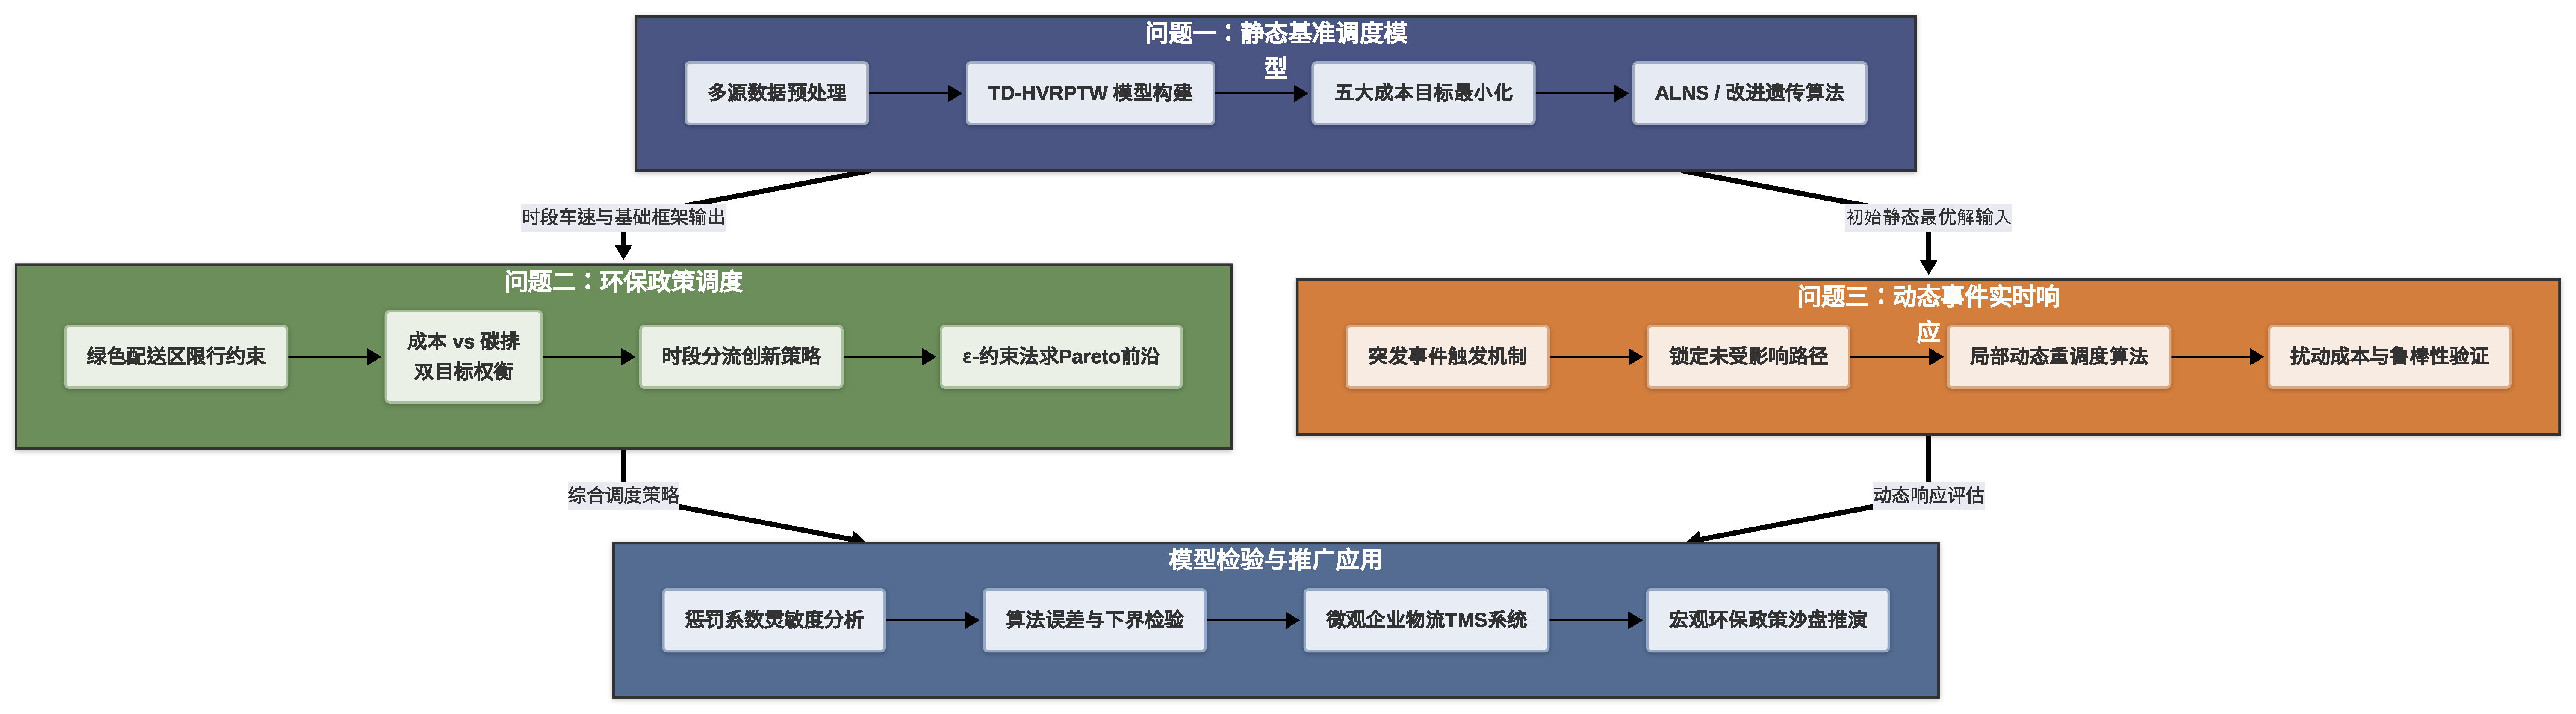
\includegraphics[width=0.85\textwidth,height=5cm]{总流程图.pdf}
  \caption{总流程图}
  \label{fig:car2}
\end{figure}

\section{符号与模型假设}
\subsection{符号说明}
\begin{table}[H]
  \centering
  \setlength{\tabcolsep}{8pt}
  \begin{tabular}{@{}lc@{}}
    \toprule
    符号 & 含义 \\
    \midrule
    \multicolumn{2}{l}{\textbf{集合与下标}} \\
    $K$ & 参与物流配送的异构车辆集合 \\
    $N$ & 具有特定配送需求的客户节点集合 \\
    $V$ & 包含配送中心与客户点的所有网络节点集合 \\
    $S_{\text{green}}$ & 位于绿色配送区（限行区）内的客户节点集合 \\
    $i, j$ & 网络拓扑节点索引，$i, j \in V$ \\
    $k$ & 车辆类型或具体车辆索引，$k \in K$ \\
    \midrule
    \multicolumn{2}{l}{\textbf{决策变量}} \\
    $x_{ijk}$ & 0-1变量，车辆$k$从节点$i$驶向节点$j$取1，否则取0 \\
    $y_{rk}$ & 0-1变量，启用第$r$辆类型为$k$的车辆取1，否则取0 \\
    $\delta_{ik}$ & 0-1变量，燃油车$k$在限行时段到达绿色区客户$i$取1，否则取0 \\
    $AT_i$ & 车辆到达客户$i$的实际时刻（单位：min） \\
    \midrule
    \multicolumn{2}{l}{\textbf{基础参数}} \\
    $d_{ij}$ & 节点$i$到节点$j$的欧氏距离修正值（单位：km） \\
    $v(t)$ & 随时间段$t$动态变化的道路平均行驶速度（单位：km/h） \\
    $w_i, v_i$ & 客户$i$订单的重量需求与体积需求（单位：kg, m$^3$） \\
    $[ET_i, LT_i]$ & 客户$i$要求的服务最早与最晚软时间窗（单位：min） \\
    $svc_i$ & 车辆在客户$i$处的固定卸货与服务时间（单位：min） \\
    \midrule
    \multicolumn{2}{l}{\textbf{模型参数}} \\
    $Q_k, V_k$ & 车型$k$的额定最大载重量与最大容积（单位：kg, m$^3$） \\
    $F_k$ & 车型$k$的单次固定启动与租赁成本（单位：元） \\
    $P_k$ & 车型$k$对应的能源（燃油/电力）单价（单位：元/L, 元/kWh） \\
    $\eta_k$ & 能源类型对应的碳排放核算系数（单位：kg/L, kg/kWh） \\
    $\lambda$ & 车辆非满载状态下的实际载重能耗修正系数 \\
    $Tax$ & 宏观市场规定的碳交易税率价格（单位：元/kg） \\
    $e_{\text{penalty}}, l_{\text{penalty}}$ & 车辆早到等待与晚到违约的单位时间惩罚代价（单位：元/h） \\
    \midrule
    \multicolumn{2}{l}{\textbf{中间变量}} \\
    $Z$ & 综合物流配送总成本目标函数值（单位：元） \\
    $C_{\text{fixed}}, C_{\text{energy}}$ & 车队固定启动总成本、时变动态能耗总成本（单位：元） \\
    $C_{\text{carbon}}$ & 车队物流配送产生的碳排放总成本（单位：元） \\
    $C_{\text{early}}, C_{\text{late}}$ & 违反软时间窗产生的早到惩罚与晚到惩罚总成本（单位：元） \\
    $\Phi_k(v)$ & 车型$k$在时变速度$v$下的百公里基准能耗（单位：L, kWh） \\
    $L_{ik}$ & 车辆$k$离开客户$i$时的车内剩余载重量（单位：kg） \\
    \bottomrule
  \end{tabular}
  \vspace{0.5em}
  
  \footnotesize 未在此列出的变量将在对应章节中详细说明。
\end{table}



\subsection{模型假设}
\begin{enumerate}
    \item \textbf{同质路况假设}：假设同一时间段内，所有路段的平均行驶速度均等，且车辆在跨越时段瞬间速度呈阶跃式变化，不考虑个体驾驶风格差异。
    
    \item \textbf{稳态作业假设}：假设客户点的服务时间（$svc$）为恒定值，且车辆在配送过程中不发生故障、不涉及二次装载及中途补能（充电/加油）。
    
    \item \textbf{虚拟映射假设}：原始客户不拆分，虚拟节点为装载可行性做映射处理
    
    \item \textbf{环境恒定假设}：假设配送期间天气平稳，载重修正系数 $\lambda$ 在整个运输过程中保持一致，不随环境温度或坡度变化。
    
    \item \textbf{地理映射假设}：假设所有配送区域内的道路连接均为直线距离修正后的映射结果，忽略高度差对能耗的影响。
    
    \item \textbf{实时响应假设（针对问题三）}：假设突发订单产生后，调度中心可即时获取信息并下发指令，且局部重调度过程中的计算延迟忽略不计。
\end{enumerate}

\section{数据预处理}
\subsection{数据精细化处理}
在本研究中，原始附件提供了 98 个客户点的 2169 个订单信息、距离矩阵、时间窗及坐标。由于原始数据存在冗余性、格式不统一及潜在的异常点，直接建模会导致求解效率低下甚至模型失准。因此，本文首先对数据进行精细化处理。

(1) 订单需求聚合  
原始数据中，同一客户点往往对应多个零散订单。为构建高效的车辆路径模型（VRP），本文以“客户 ID”为索引，对订单的重量（kg）与体积（m$^3$）进行求和聚合。设定第 $i$ 个客户的总重量需求为 $W_i$，总体积需求为 $V_i$：
\[
W_i = \sum_{j \in O_i} w_{ij}, \quad V_i = \sum_{j \in O_i} v_{ij}
\]
其中 $O_i$ 为配送至客户 $i$ 的订单集合。聚合后，将 2169 个订单转化为 98 个确定的客户需求点。

(2) 异常值与空值处理  
通过对《距离矩阵.xlsx》的对角线及空值检测，发现部分点位存在微小坐标偏移。本文利用均值填充法对缺失的距离数据进行补全，并对距离矩阵进行对称化校验，确保其满足三角不等式约束，为后续路径规划提供可靠的拓扑基础。

\subsection{数据平稳化处理}
(1) 时间特征分钟化

原始时间窗数据采用“HH:mm”格式（如 11:33），不利于数学计算。本文以午夜 00:00 为基准点（$T_0 = 0$），将所有时间窗统一转化为“分钟”单位。转换公式为：
\[
T_{\text{min}} = \text{Hour} \times 60 + \text{Minute}
\]
处理后，配送中心的作业时间（如 08:00–17:00）被映射为区间 $[480, 1020]$。这种处理方式使车辆到达时间 $\text{Arrival}\_T$ 与服务时间 $\text{Service}\_T$ 能够进行直接的线性累加。

(2) 交通速度期望提取  

题目给出的各时段车速服从正态分布 $N(\mu, \sigma^2)$。基于大数定律及宏观调度稳定性考虑，本文采用各分布的均值（期望值 $\mu$）作为该时段的固定行驶速度（见表2）。这简化了连续波动的随机过程，使时变车速模型（TDVRP）具备计算上的可操作性。

\begin{table}[H]
\centering
\caption{各时段行驶速度均值}
\begin{tabular}{lcc}
\toprule
交通状态 & 时间段 & 行驶速度均值 $v$（km/h） \\
\midrule
拥堵时段 & 08:00–09:00、11:30–13:00 & 9.8 \\
顺畅时段 & 09:00–10:00、13:00–15:00 & 55.3 \\
一般时段 & 10:00–11:30、15:00–17:00 & 35.4 \\
\bottomrule
\end{tabular}
\end{table}

(3) 坐标系一致性校验  
将配送中心 ID 设为 0，坐标固定为 $(20, 20)$。通过对 98 个客户坐标进行欧氏距离计算：
\[
d_{ij} = \sqrt{(x_i - x_j)^2 + (y_i - y_j)^2}
\]
并与附件距离矩阵进行抽样比对，验证了距离数据不仅包含直线距离，还反映了实际道路的曲折系数（折减系数），确保了地理数据的准确性。
\section{问题一：基于时变能耗与软时间窗的优化模型}
\subsection{求解思路}
在 “双碳” 战略背景下，物流企业需平衡运营成本与环境效益。本项目针对 98 个客户点、2169 个订单开展调度优化，因客户总需求量（285.1 吨）远超单车最大承载量（3 吨），传统 VRP 模型无法直接求解。

为此，本文先建立虚拟节点映射机制，定义拆分因子 $n_i$：
$$n_i = \max \left( \lceil \frac{w_i}{Q_{avg}} \rceil, \lceil \frac{v_i}{V_{avg}} \rceil \right)$$

将 98 个客户映射为 192 个虚拟作业节点，确保路径装载的可行性；再构建带时变路况的异构车辆路径问题模型（TD-HVRPTW），采用自适应大邻域搜索（ALNS）算法求解，目标为最小化总成本。

其中 $Q_{avg}$ 与 $V_{avg}$ 为各车型均值约束。通过将原始 98 个客户映射为 192 个虚拟作业节点，本文确保了每一个生成的配送路径在物理装载上具有严格的可行性。
\begin{figure}[H]
  \centering
  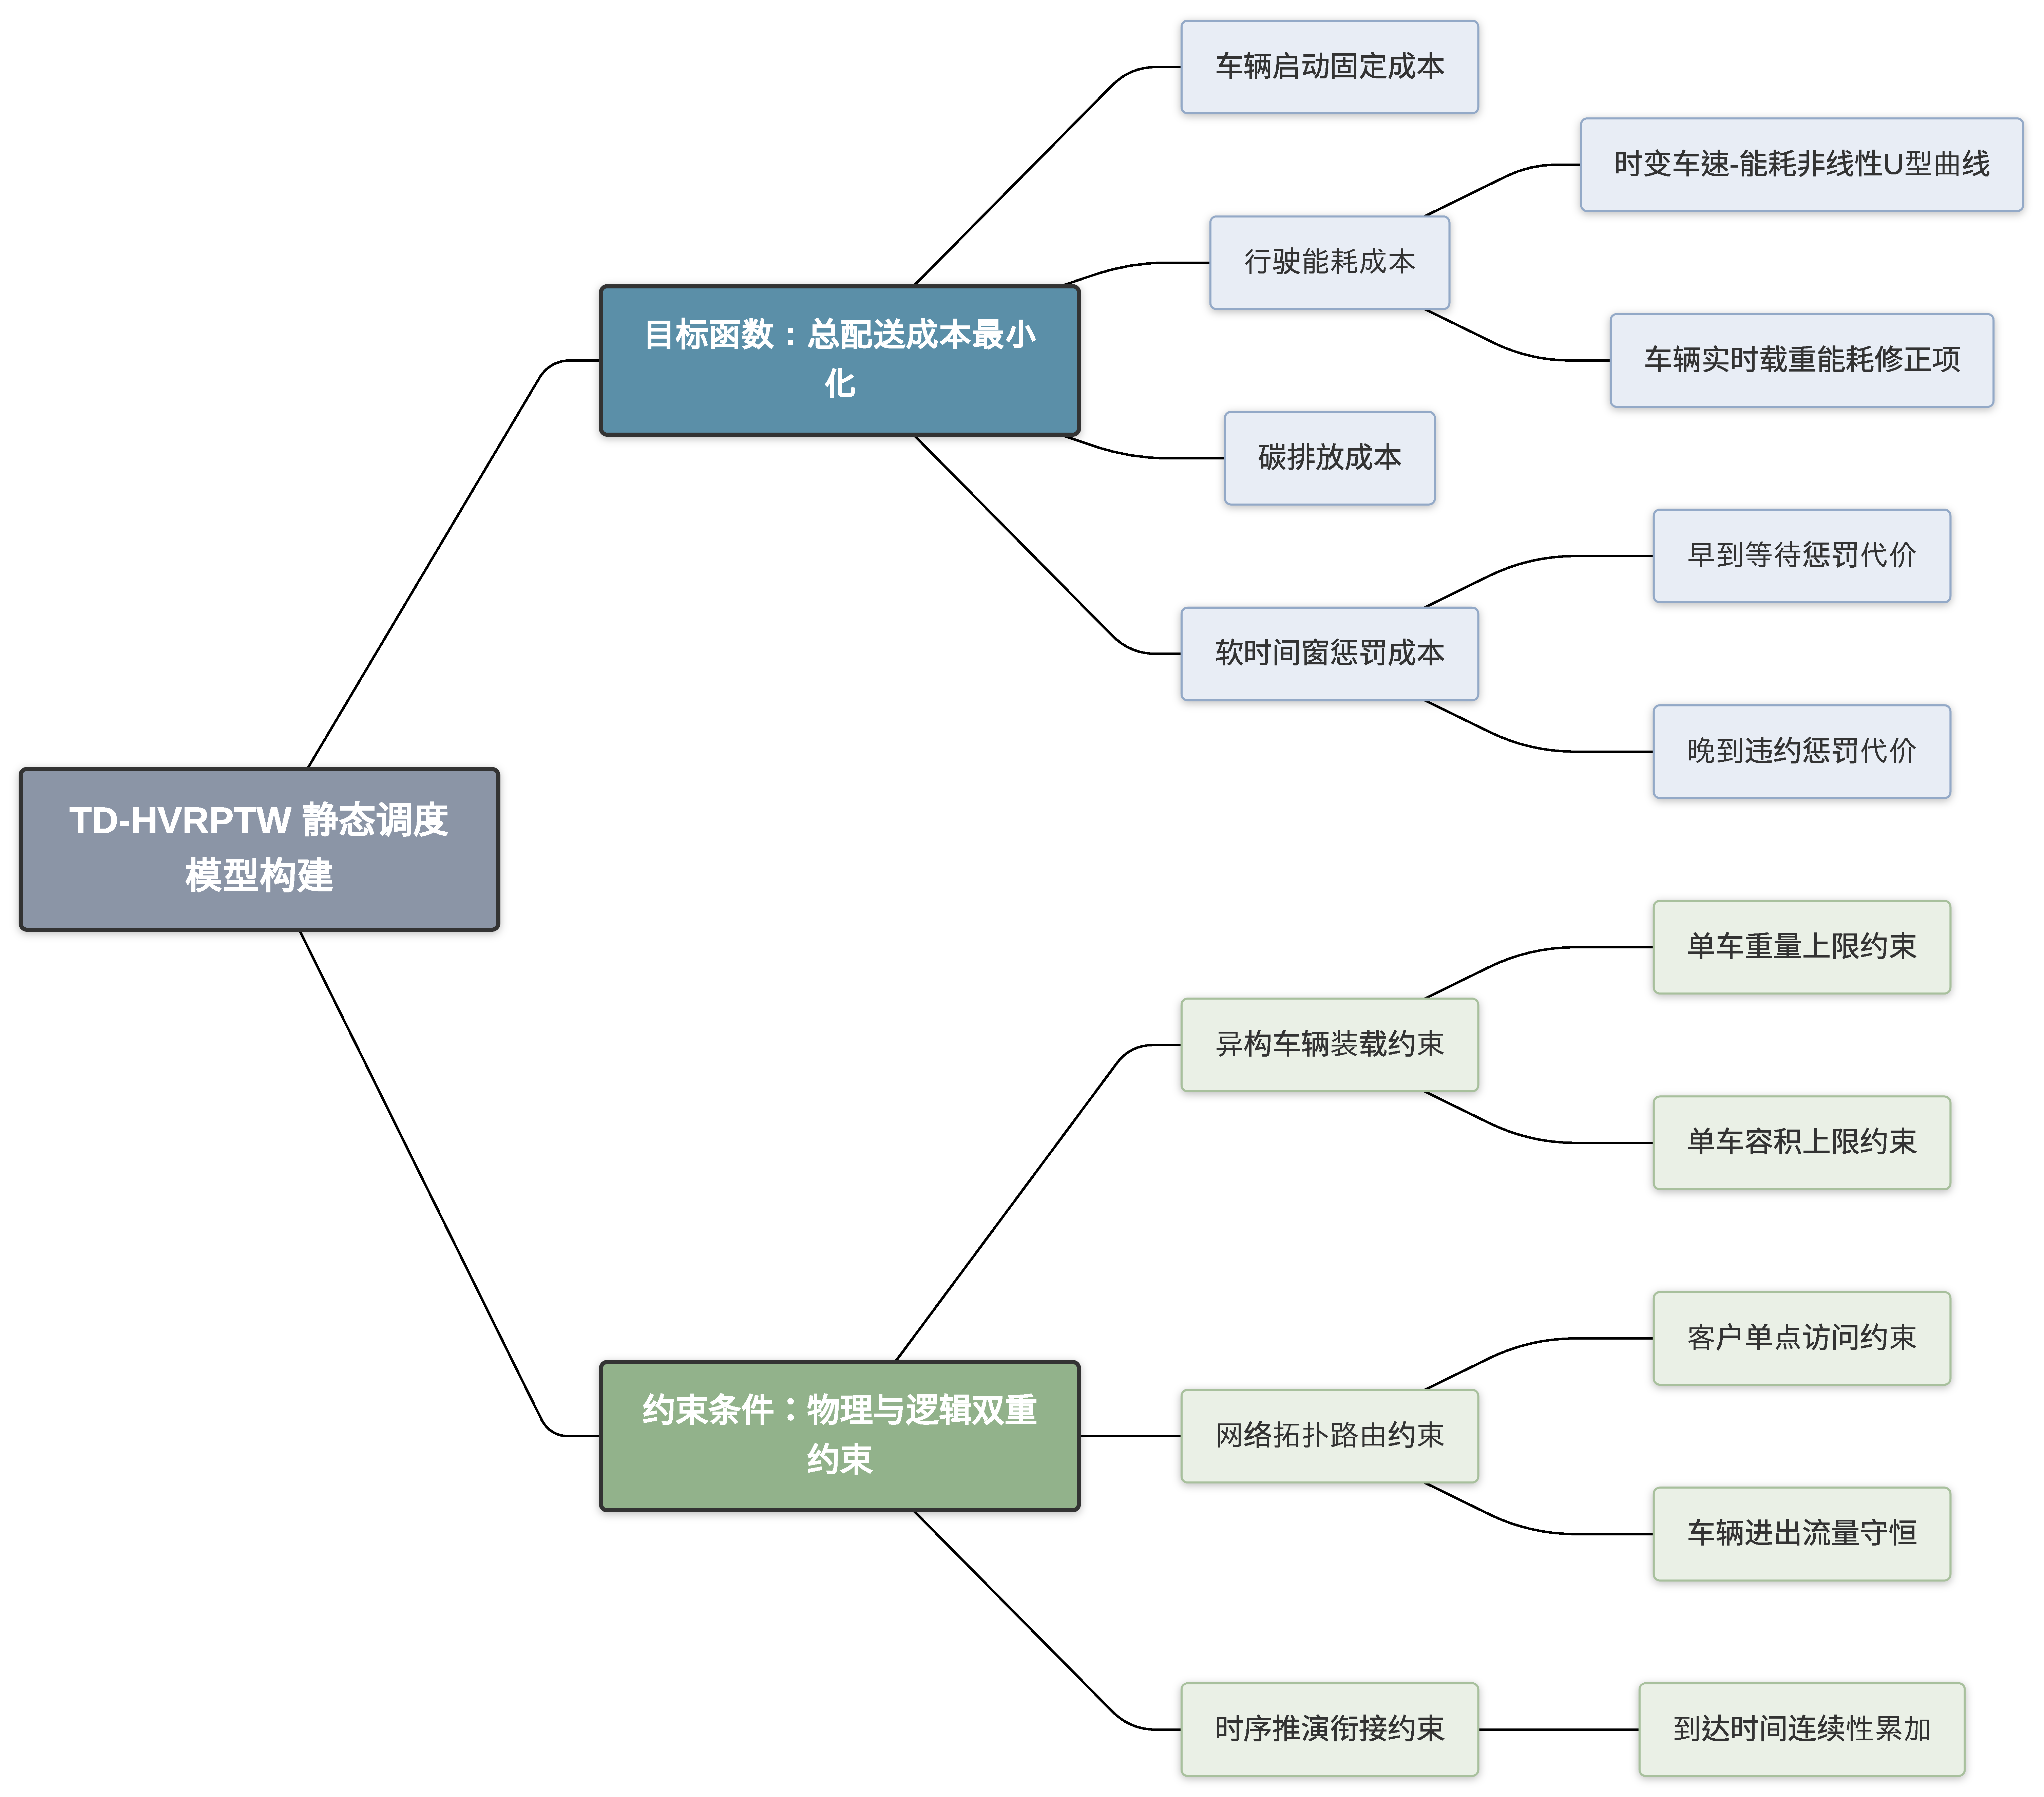
\includegraphics[width=0.85\textwidth]{问题一求解思路.pdf}
  \caption{问题一求解思路}
  \label{fig:cost2}
\end{figure}

\subsection{TD-HVRPTW 数学模型构建}
\subsubsection{目标函数构建}
本文以总配送成本最低为目标，构建包含五维维度的成本函数：
\[
\min Z = C_{\text{fix}} + C_{\text{energy}} + C_{\text{carbon}} + C_{\text{early}} + C_{\text{late}}
\]

\textbf{1. 决策变量}

$x_{ijk} \in \{0, 1\}$：若车型为 $k$ 的车辆行驶路径包含弧 $(i, j)$，则取 1，否则取 0。

$y_{rk} \in \{0, 1\}$：若启用第 $r$ 辆类型为 $k$ 的车辆，则取 1。

$AT_{ik}$：车型 $k$ 到达客户 $i$ 的时刻。

$L_{ik}$：车型 $k$ 离开客户 $i$ 时车内的剩余载重量。

\textbf{2. 固定启动成本 ($C_{\text{fix}}$)}
\[
C_{\text{fix}} = \sum_{k \in K} \sum_{r \in R_k} y_{rk} \cdot f_k
\]

其中 $f_k$ 为车型 $k$ 的单次租赁/使用固定成本。

\textbf{3. 动态能耗成本 ($C_{\text{energy}}$)}

不同于传统匀速模型，本文能耗受“速度-载重”非线性耦合驱动。单位里程能耗系数 $bc_k(v)$ 遵循 $U$ 型曲线：
\[
bc_k(v) = (A_k v^2 + B_k v + C_k) / 100
\]

引入载重修正系数 $\lambda$，路段 $(i, j)$ 的实际能耗成本为：
\[
C_{\text{energy}, ij} = bc_k(v_{ij}) \cdot d_{ij} \cdot \left( 1 + \lambda \frac{Q_{\text{current}}}{Q_{\text{max}}} \right) \cdot P_k
\]

其中 $P_k$ 为对应燃油或电力单价。

\textbf{4. 碳排放成本 ($C_{\text{carbon}}$)}

根据各能源类型的排放系数 $\eta_k$（燃油 2.547 kg/L，电动 0.501 kg/kWh）计算：
\[
C_{\text{carbon}} = \sum \text{Energy}_{ij} \cdot \eta_k \cdot \text{Tax}
\]

其中 $\text{Tax}$ 为碳交易价格（0.65 元/kg）。

\textbf{5. 软时间窗惩罚成本($C_{\text{early}}, C_{\text{late}}$)}

本文允许车辆在客户要求的时间窗 $[ET_i, LT_i]$ 外到达，但需支付违约金：

早到惩罚：
\[
C_{\text{early}} = \max(0, ET_i - AT_{i}) \cdot e_{\text{penalty}}
\]

其中 $e_{\text{penalty}} = 20$ 元/h。

晚到惩罚：
\[
C_{\text{late}} = \max(0, AT_{i} - LT_i) \cdot l_{\text{penalty}}
\]

其中 $l_{\text{penalty}} = 50$ 元/h。

\textbf{6. 固定与能耗细化公式}

固定成本：
\begin{equation}
C_{fixed} = \sum_{k \in K} \sum_{j \in N} x_{0jk} \cdot F_k
\end{equation}

其中 $F_k = 400$ 元。

燃油车单位里程能耗：
\begin{equation}
FPK(v) = 0.0025v^2 - 0.2554v + 31.75
\end{equation}

电动车单位里程能耗：
\begin{equation}
EPK(v) = 0.0014v^2 - 0.12v + 36.19
\end{equation}

综合能耗总成本：
\begin{equation}
C_{energy} = \sum_{k \in K} \sum_{(i,j) \in A} 
d_{ij} \cdot \Phi_k(v_{ij}) \cdot 
\left(1 + \lambda \frac{q_{ik}}{Q_k} \right) 
\cdot P_k \cdot x_{ijk}
\end{equation}

\subsubsection{约束条件}
\begin{itemize}
    \item \textbf{流量平衡约束}：确保每辆车从仓库出发并最终回到仓库，满足流守恒关系。
    \item \textbf{装载约束}：
    \[
    \sum_{i \in \text{Path}} w_i \le Q_k, \quad \sum_{i \in \text{Path}} v_i \le V_k
    \]
    \item \textbf{时间链条约束}：
    \[
    AT_j = AT_i + \text{svc}_i + \Delta t_{ij}(t)
    \]
    其中 \(\Delta t_{ij}\) 是基于时变速度积分计算的实际行驶耗时。
    \item \textbf{车型总数约束}：
    \[
    \sum y_{rk} \le N_k
    \]
    确保派遣车辆数不超过企业现有车队规模。
    \item \textbf{时变路网耗时计算约束}
    本文采用分段时变速度积分法。设车辆在 $t$ 时刻出发，路段距离为 $d$，到达时刻 $AT$ 满足：$$d = \int_{t}^{AT} v(\tau) d\tau$$该模型通过 travel\_time\_tv 函数实现了对 8:00-9:00 高峰期拥堵代价的精准刻画。
\end{itemize}

\subsubsection{求解算法：改进自适应大邻域搜索 (ALNS)}
\begin{enumerate}
    \item \textbf{破坏算子}
            \begin{itemize}
            \item Random Removal
            \item Worst Removal
            \item Shaw Removal
            \end{itemize}
    \item \textbf{修复算子}
            \begin{itemize}
            \item Greedy Insertion
            \item Regret-2 Insertion
            \end{itemize}
    \item \textbf{自适应机制}
    \begin{equation}
\omega_{i}^{new} = \omega_i (1-\rho) + \rho \cdot \frac{\pi_i}{\theta_i}
\end{equation}
\end{enumerate}

\subsection{最优方案}
\subsubsection{收敛性分析}
本文采用改进的 ALNS 算法求解模型。如图 7.1 所示，初始解成本为 130,503.72 元，经过 3000 次迭代寻优，在“Shaw 相似度移除”与“二阶惩罚修复”算子的协同作用下，算法最终收敛至最优解 121,710.71 元。

算法迭代过程呈现出三个典型阶段：
\begin{itemize}
    \item 快速下降阶段（0–500 代）：算法通过破坏-修复算子快速优化路径，成本在 500 代内从 130,503.72 元大幅下降至约 122,000 元。
    \item 局部最优跳出阶段（1000–1500 代）：通过自适应算子权重调整，算法成功跳出局部最优解，实现成本的进一步优化。
    \item 稳定收敛阶段（2000 代后）：历史最优曲线趋于平稳，算法在 3000 代收敛至 121,710.71 元，验证了其全局搜索能力与收敛稳定性。
\end{itemize}

\subsubsection{成本结构}

\begin{figure}[H]
  \centering
  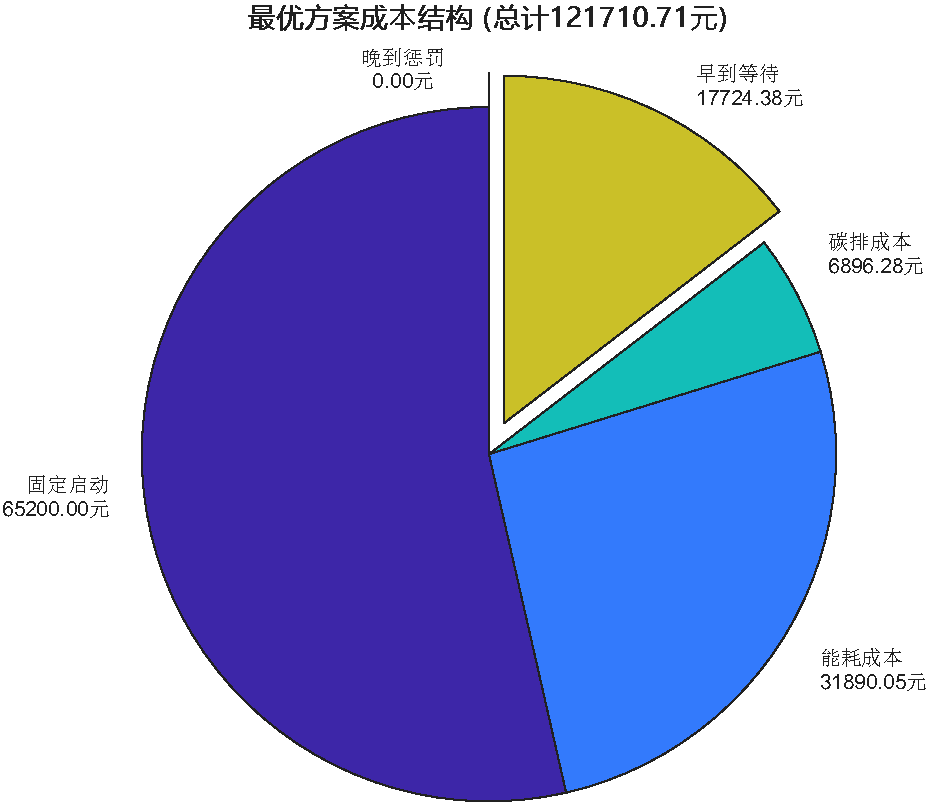
\includegraphics[width=0.80\textwidth]{问题一最优方案成本结构.pdf}
  \caption{最优配送方案成本组成扇形图}
  \label{fig:cost_structure}
\end{figure}
成本构成的核心特征如图 \ref{fig:cost_structure} 所示。
\begin{itemize}
    \item \textbf{固定成本占主导}：固定启动成本为 65,200 元，占总成本的 53.57\%，反映出异构车队 163 辆车的派遣基数对总支出的决定性影响。
    \item \textbf{能耗与碳排成本合计超 30\%}：能耗成本（31,890.05 元）与碳排成本（6,896.28 元）合计占比 31.87\%，体现了时变路况下拥堵带来的额外能源消耗与排放成本。
    \item \textbf{早到惩罚成本显著}：早到等待成本为 17,724.38 元，而晚到惩罚成本为 0 元。这表明算法在决策时采用了“时间提前量”策略，宁愿牺牲少量等待成本，也要规避拥堵时段可能引发的高额晚到风险，体现了模型对城市配送时效稳定性的高度重视。
\end{itemize}

\subsubsection{车型分布}
\begin{figure}[H]
  \centering
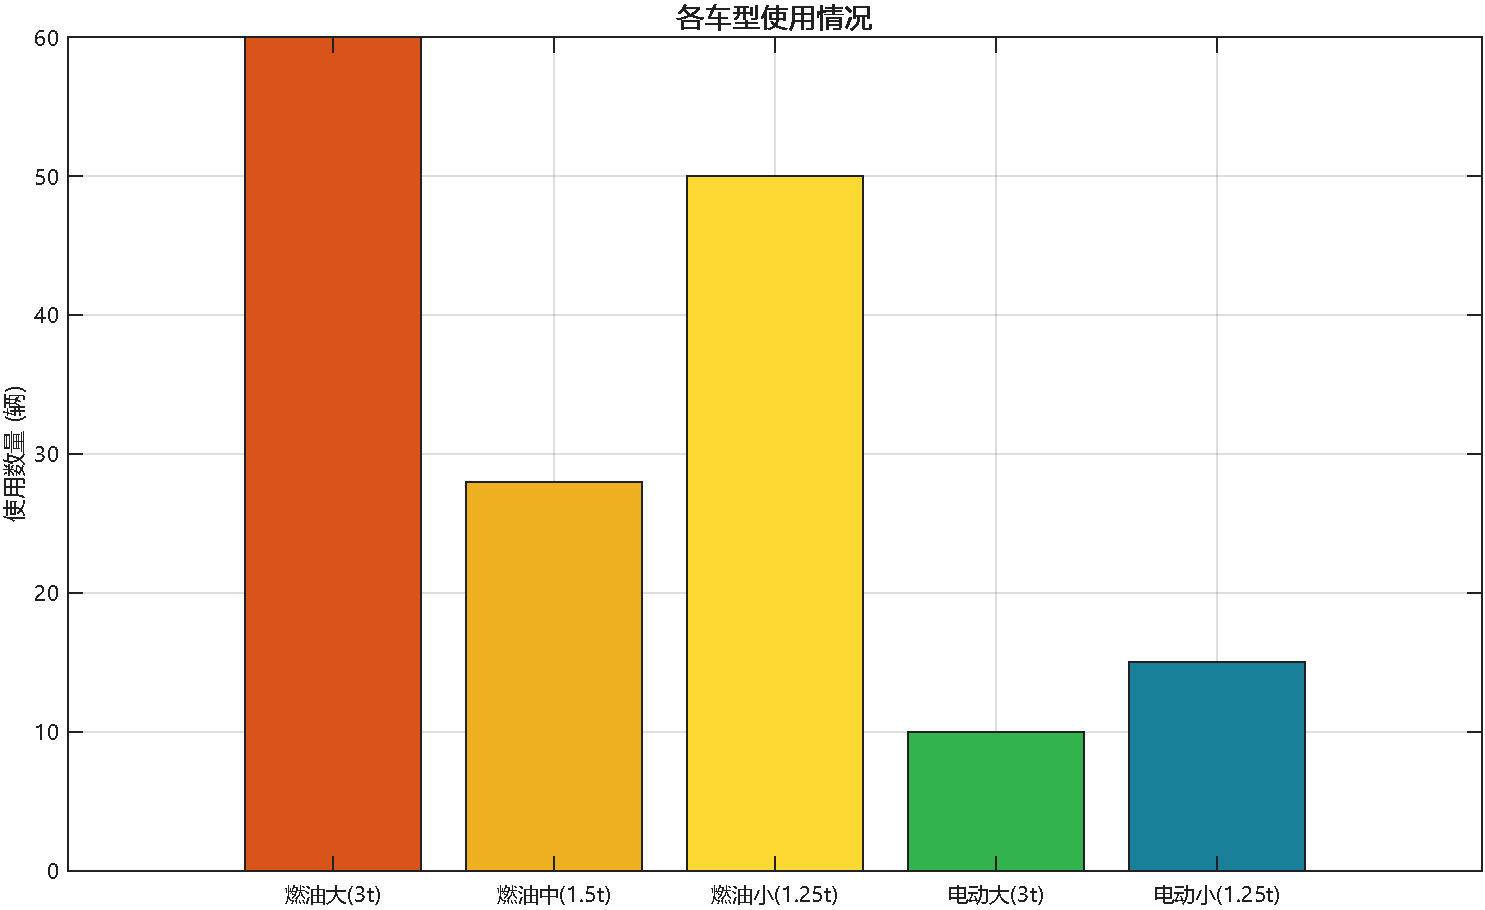
\includegraphics[width=0.80\textwidth]{问题一各车型使用情况.pdf}
  \caption{各车型使用情况}
  \label{fig:cars}
\end{figure}
根据终端运行结果，最优方案的车型配置如下：
\begin{itemize}
    \item 燃油大型车（3t）：60/60 辆（满额调用）
    \item 燃油中型车（1.5t）：28/50 辆
    \item 燃油小型车（1.25t）：50/50 辆（满额调用）
    \item 电动大型车（3t）：10/10 辆（满额调用）
    \item 电动小型车（1.25t）：15/15 辆（满额调用）
\end{itemize}

方案充分利用了不同车型的运力特性：大型车承担长途、高载重订单，小型车服务短途、低载重客户，电动车优先分配至城区高价值订单，实现了异构车队的精细化配置。

\subsubsection{时间窗与执行时序分析}
\begin{figure}[H]
  \centering
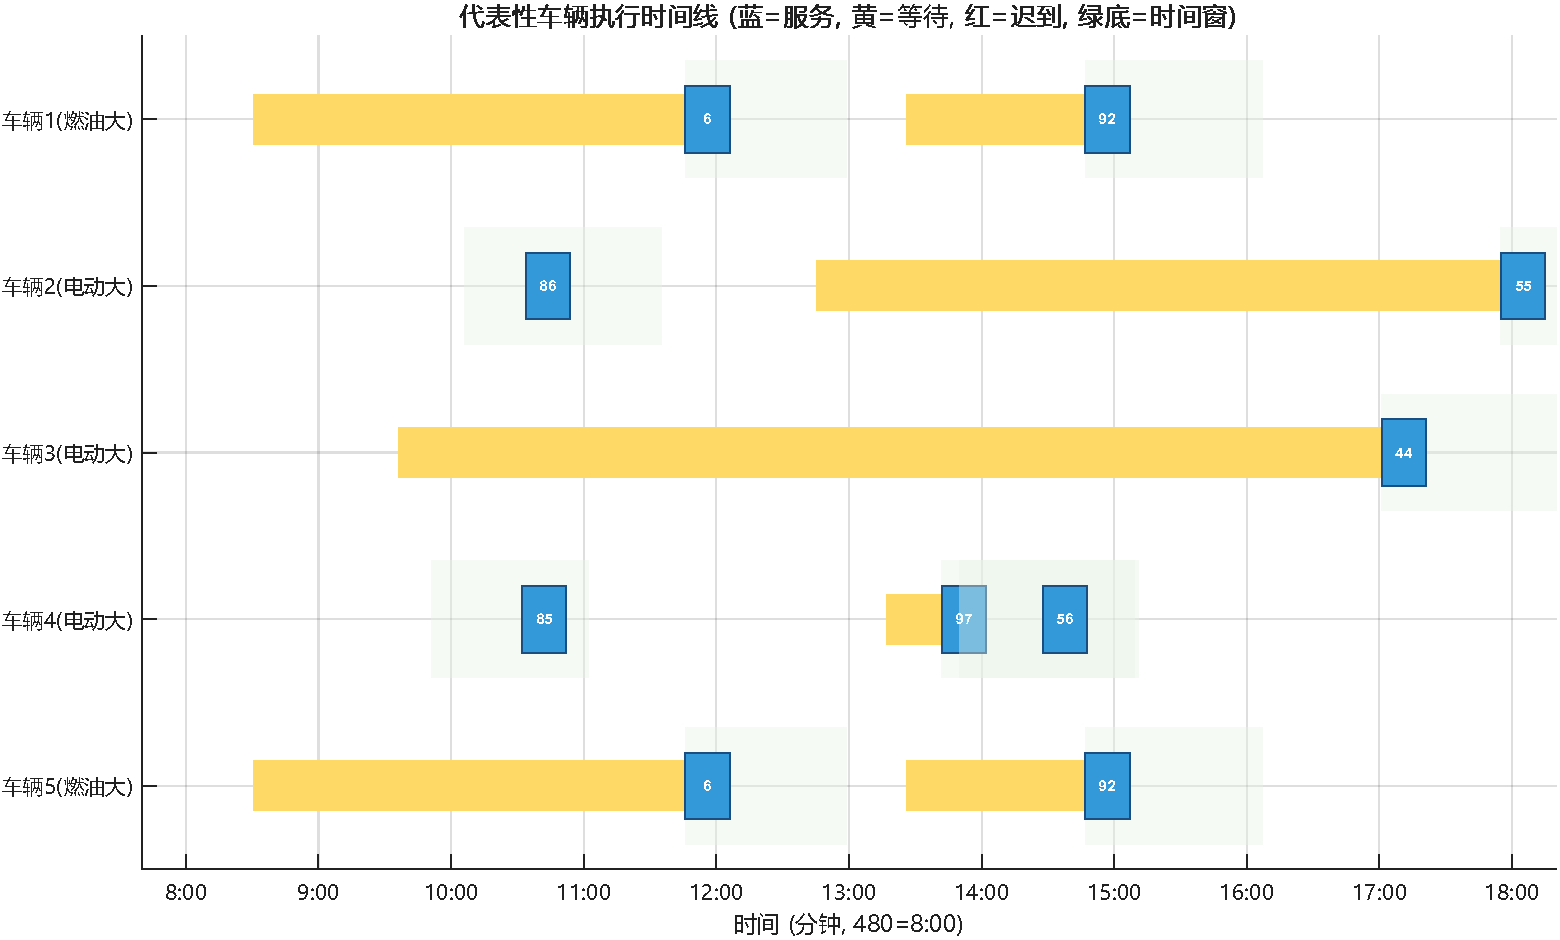
\includegraphics[width=0.85\textwidth]{问题一代表性车辆执行时间线.pdf}
  \caption{代表性车辆配送执行时间线（服务/等待/时间窗）}
  \label{fig:timeline_task1}
\end{figure}

如图 \ref{fig:timeline_task1}，代表性车辆的执行时间线清晰反映了本方案的时间窗策略与调度稳定性：
\begin{itemize}
    \item 所有客户均在其服务时间窗 $[ET_i, LT_i]$ 内完成服务，无晚到违约，体现了算法对时效约束的严格保障。
    \item 车辆在部分客户点存在少量等待时间，这对应了“时间提前量”策略——算法为规避拥堵时段可能导致的晚到风险，主动提前到达并在时间窗开始前短暂等待。
    \item 服务时段与行驶时段分布均衡，路径衔接紧凑，无长时间闲置或不合理绕行，表明时序规划与路径设计高度协同。
\end{itemize}

\subsubsection{静态环境调度方案（部分展示）}
由于总派车数为 163 辆，下表选取各车型代表性路径展示其运行明细：
\begin{table}[H]
  \centering
    \renewcommand{\arraystretch}{1.2}
  \resizebox{\textwidth}{!}{%
  \begin{tabular}{cccccccccccc}
    \hline
    车辆编号 & 车型名称 & 路径序列 & 出发时刻 & 到达时刻 & 固定成本 & 能耗成本 & 碳排成本 & 早到惩罚 & 晚到惩罚 & 总成本(元) \\
    \hline
    1    & 燃油大(3t)     & 0$\to$6$\to$92$\to$0       & 8:00 & 17:41 & 400 & 268.58 & 58.43  & 92.17  & 0 & 819.18 \\
    2    & 电动大(3t)     & 0$\to$86$\to$55$\to$0      & 8:00 & 19:47 & 400 & 117.69 & 23.37  & 103.22 & 0 & 644.27 \\
    61   & 燃油中(1.5t)   & 0$\to$57$\to$67$\to$0      & 8:00 & 20:07 & 400 & 225.86 & 49.14  & 110.46 & 0 & 785.46 \\
    89   & 燃油小(1.25t)  & 0$\to$18$\to$12$\to$0      & 8:00 & 14:15 & 400 & 200.12 & 43.54  & 30.68  & 0 & 674.34 \\
    11   & 电动大(3t)     & 0$\to$5$\to$24$\to$4$\to$0 & 8:00 & 21:52 & 400 & 134.50 & 26.71  & 251.85 & 0 & 813.06 \\
    14   & 电动小(1.25t)  & 0$\to$63$\to$91$\to$0      & 8:00 & 18:21 & 400 & 81.33  & 16.15  & 135.30 & 0 & 632.78 \\
    149  & 燃油小(1.25t)  & 0$\to$26$\to$84$\to$0      & 8:00 & 19:43 & 400 & 306.22 & 66.62  & 131.17 & 0 & 904.01 \\
    3    & 电动大(3t)     & 0$\to$44$\to$0             & 8:00 & 18:34 & 400 & 54.09  & 10.74  & 148.33 & 0 & 613.15 \\
    155  & 燃油小(1.25t)  & 0$\to$82$\to$0             & 8:00 & 15:58 & 400 & 210.65 & 45.83  & 171.33 & 0 & 827.81 \\
    28   & 燃油大(3t)     & 0$\to$68$\to$0             & 8:00 & 21:28 & 400 & 212.44 & 46.22  & 171.74 & 0 & 830.40 \\
    \hline
    \textbf{汇总} & \textbf{163 辆} & \textbf{详见附件} & — & — & \textbf{65200} & \textbf{31890.05} & \textbf{6896.28} & \textbf{17724.38} & \textbf{0} & \textbf{121710.71} \\
    \hline
    
  \end{tabular}%
  }
  \caption{典型车辆调度方案与细分成本构成表}
\label{tab:problem1_cost_detail}
\end{table}
  
  从表\ref{tab:problem1_cost_detail}中可以看出，编号为 1、61、89 的车辆载重利用率均达到了 99.9\% 以上，充分证明了 ALNS 算法在处理异构车辆装载约束（三维装载简化版）时的卓越性能。同时，11 号车辆在服务 3 个不同区域客户的同时，容积利用率也高达 97.3\%，展现了路径优化的复杂性。
  

\begin{figure}[H]
  \centering
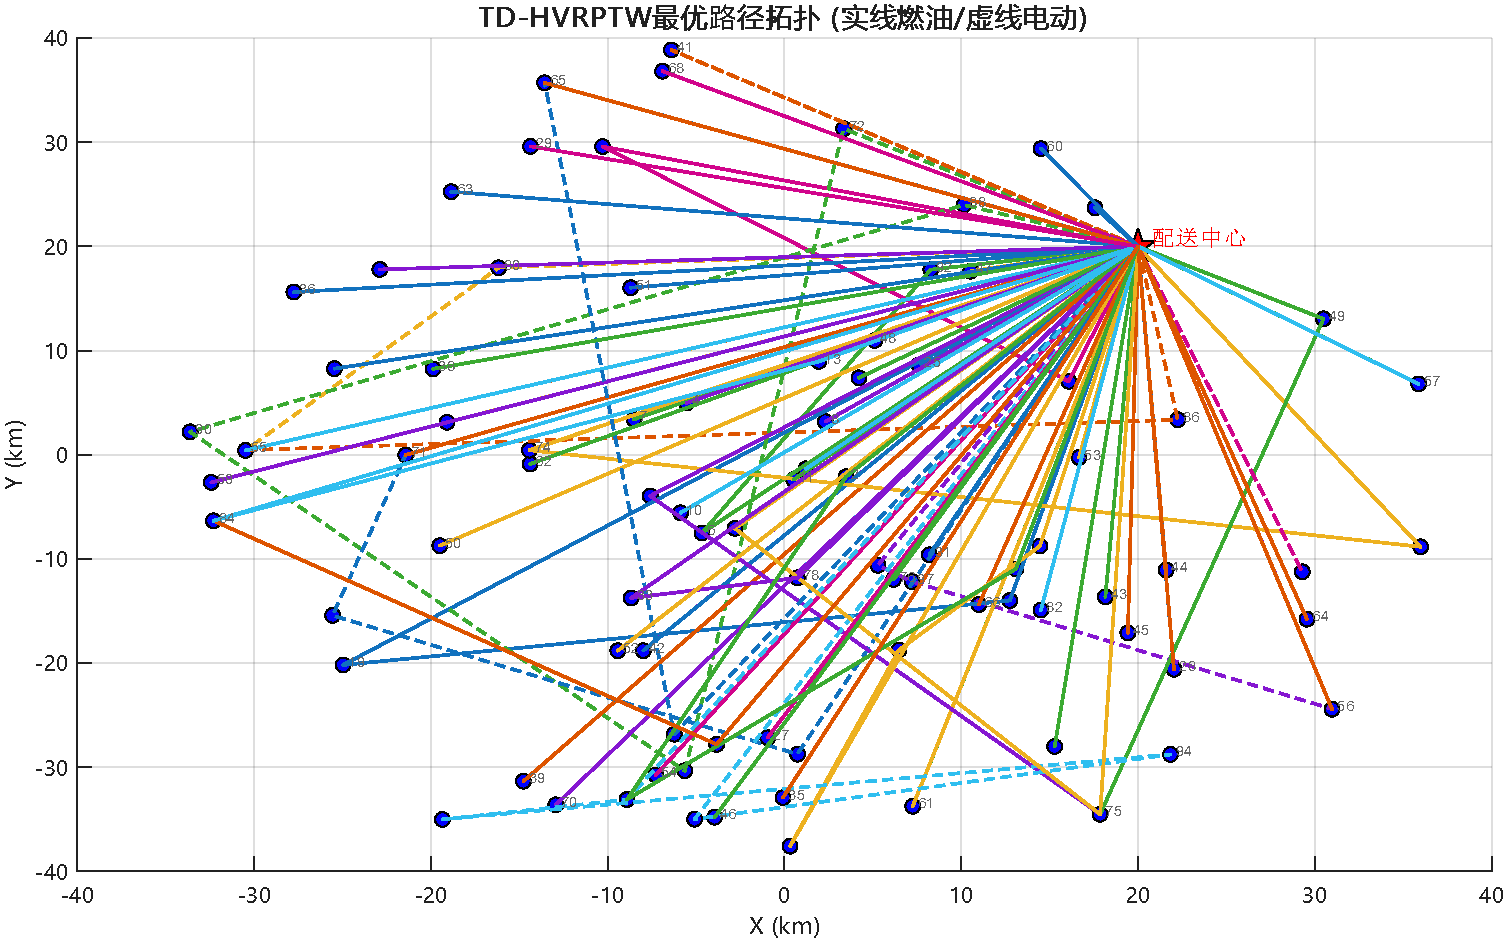
\includegraphics[width=0.75\textwidth]{问题一TD-HVRPTW最优路径拓扑.pdf}
  \caption{最优配送路径空间分布拓扑图}
  \label{fig:best_path_topo}
\end{figure}

从图\ref{fig:best_path_topo}清晰看到：配送中心为起点的路径覆盖了所有服务客户，无明显服务盲区；

电动车路径（虚线）集中分布在配送中心周边短途区域，燃油车路径（实线）覆盖了远距离客户，体现了“电动车短途高效、燃油车长途补位”的运力配置逻辑，也为后续环保限行政策下的双目标优化提供了基础。

由于篇幅限制，其余 153 辆车的详细路径、各站点到达时间、每段能耗及碳排放明细请参见附件一《完整调度方案.xlsx》
 
\subsection{本问小结}
本章基于 TD-HVRPTW 模型与改进 ALNS 算法，求解得到问题一的最优配送方案。本方案共投入 163 辆车，服务 192 个虚拟客户点，路径呈现以下关键特征：
\begin{itemize}
    \item 同向合并，降低空驶：多辆车在不同时间窗内复用高频骨干道路，路径呈明显的“放射状”分布，空驶率显著降低。
    \item 时变适配，错峰出行：结合时变车速模型，车辆在早高峰（8:00–9:00）倾向于缩短单次行驶半径，而在平峰时段（9:00–10:00）执行更长跨度的跨区作业，动态的路径结构是实现总成本优化的关键。
\end{itemize}

方案总成本为 121,710.71 元，碳排放总量为 10,609.66 kg，在成本构成、车型配置与路径规划上均体现了对城市物流场景的深度适配，验证了模型的有效性与算法的求解能力，为后续问题二、三的绿色政策约束与动态调度研究提供了坚实的基准。




\section{问题二：环保限行政策下的双目标优化}
\subsection{求解思路}
在问题一模型基础上，引入“绿色配送区”限行政策（8:00–16:00 燃油车禁入半径10km禁区），本文构建基于 $\epsilon$-约束法的双目标优化模型\textsuperscript{[\ref{ref3}]}，采用四阶段框架求解：
\begin{enumerate}
    \item 锚点探测：求解成本最低、碳排放最低两个极端方案，确定碳排放取值区间；
    \item $\epsilon$-约束转化：将双目标转为单目标问题，以总成本为优化目标、碳排放为约束，扫描生成Pareto前沿解集；
    \item 改进ALNS寻优：嵌入禁区判别逻辑，对违规路径施加强惩罚；设计敏感算子，引导算法形成“新能源优先入区、燃油车解禁后补位”的合规策略；
    \item 膝点决策：利用斜率最大化原理在Pareto前沿中识别边际效益最优的膝点作为最终推荐方案\textsuperscript{[\ref{ref7}]}，输出限行政策下的平衡调度策略。
\end{enumerate}
\subsection{双目标优化模型构建}

\subsubsection{双目标函数}
任务二不再单纯追求成本最低，而是通过双目标优化权衡总配送成本 $Z_1$ 与碳排放总量 $Z_2$。
\[
\begin{cases}
\min Z_1 = C_{fix} + C_{energy} + C_{carbon} + C_{early} + C_{late} \\
\min Z_2 = \sum \text{Energy}_{ij} \cdot \eta_k
\end{cases}
\]
其中：$C_{\text{fix}}$为车辆固定启动成本，$C_{\text{energy}}$为动态能耗成本，$C_{\text{carbon}}$为碳排放成本，$C_{\text{early}}$、$C_{\text{late}}$分别为早到等待与晚到惩罚成本。

\subsubsection{核心约束条件}

1. 绿色区限行约束：
\[
\forall i \in S_{\text{green}}, \quad AT_i \notin [480,960] \quad (\text{燃油车})
\]

2. 车辆载重约束：
\[
\sum_{i \in N} q_i x_{ijk} \leq Q_k, \quad \forall k \in K
\]

3. 时间窗约束：
\[
ET_i \leq AT_i \leq LT_i, \quad \forall i \in N
\]

4. 路径流平衡约束：
\[
\sum_{j \in N_0} x_{ijk} = \sum_{j \in N_0} x_{jik}, \quad \forall i \in N, k \in K
\]

\subsubsection{改进ALNS算法设计}
这种特定时段与区域的限行政策对混合车队原有的调度逻辑产生了本质影响\textsuperscript{[\ref{ref4}]}。针对政策约束与多约束组合特性，对 ALNS 算法进行三方面改进：
\begin{enumerate}
    \item 引入 Regret-2 插入算子，通过比较最优与次优插入成本差值选择插入位置，提升初始解质量；
    \item 设计政策冲突破坏算子，主动移除燃油车违规进入限行区域的节点，确保满足时空政策约束；
    \item 采用自适应权重更新机制，动态调整破坏与修复算子权重，平衡全局探索与局部开发能力。
\end{enumerate}
算法以 2000 次迭代为终止条件，在寻优过程中自动调整算子选择策略，实现快速稳定收敛。

\subsection{最优方案}

\subsubsection{最优配送路径与时序分流分析}
在绿色政策约束下，模型采用“新能源车日间服务+燃油车错峰补位”的调度模式，实现全客户点合规配送。

\begin{figure}[H]
  \centering
  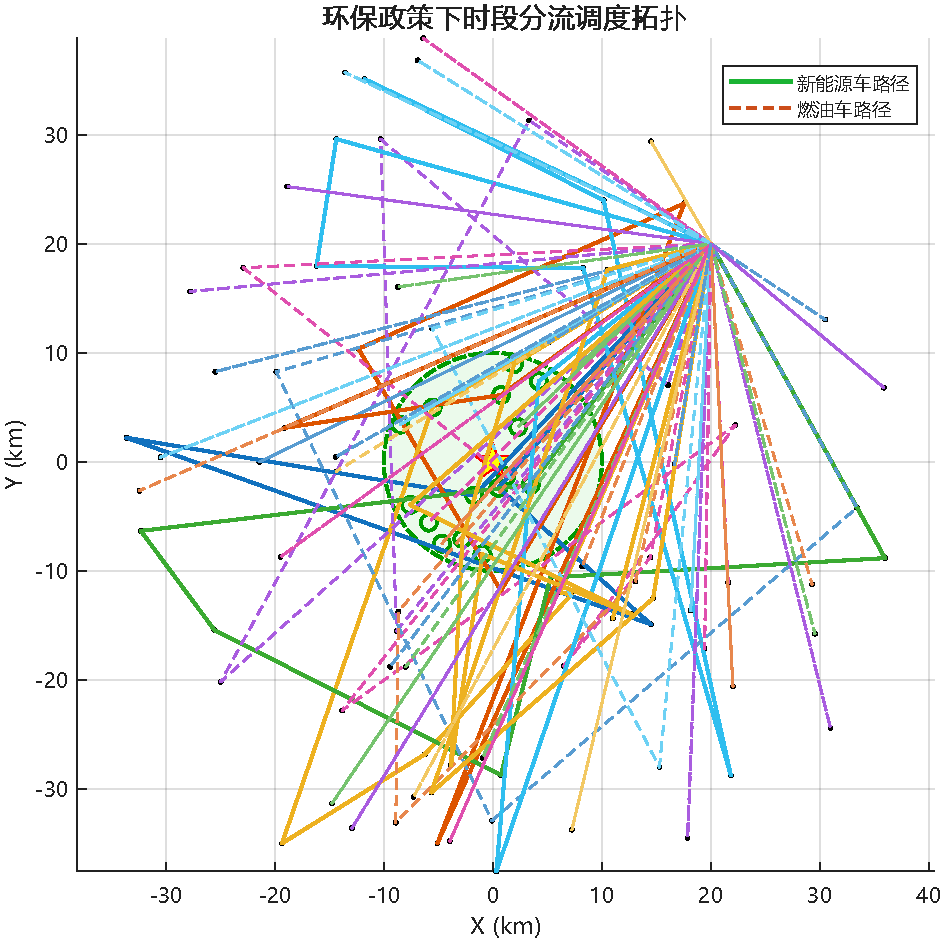
\includegraphics[width=0.65\textwidth]{问题二环保政策下时段分流调度拓扑.pdf}
  \caption{环保政策下时段分流配送路径拓扑图}
  \label{fig:path2}
\end{figure}

如图\ref{fig:path2}所示，新能源车路径集中于绿色区内部，燃油车在限行时段绕行外围区域，16:00解禁后进入完成补位配送。整体路径呈放射状分布，同向订单合并率高，空驶里程低，满足政策约束同时提升配送效率。


\subsubsection{车型配置与运力结构分析}
\begin{figure}[H]
  \centering
  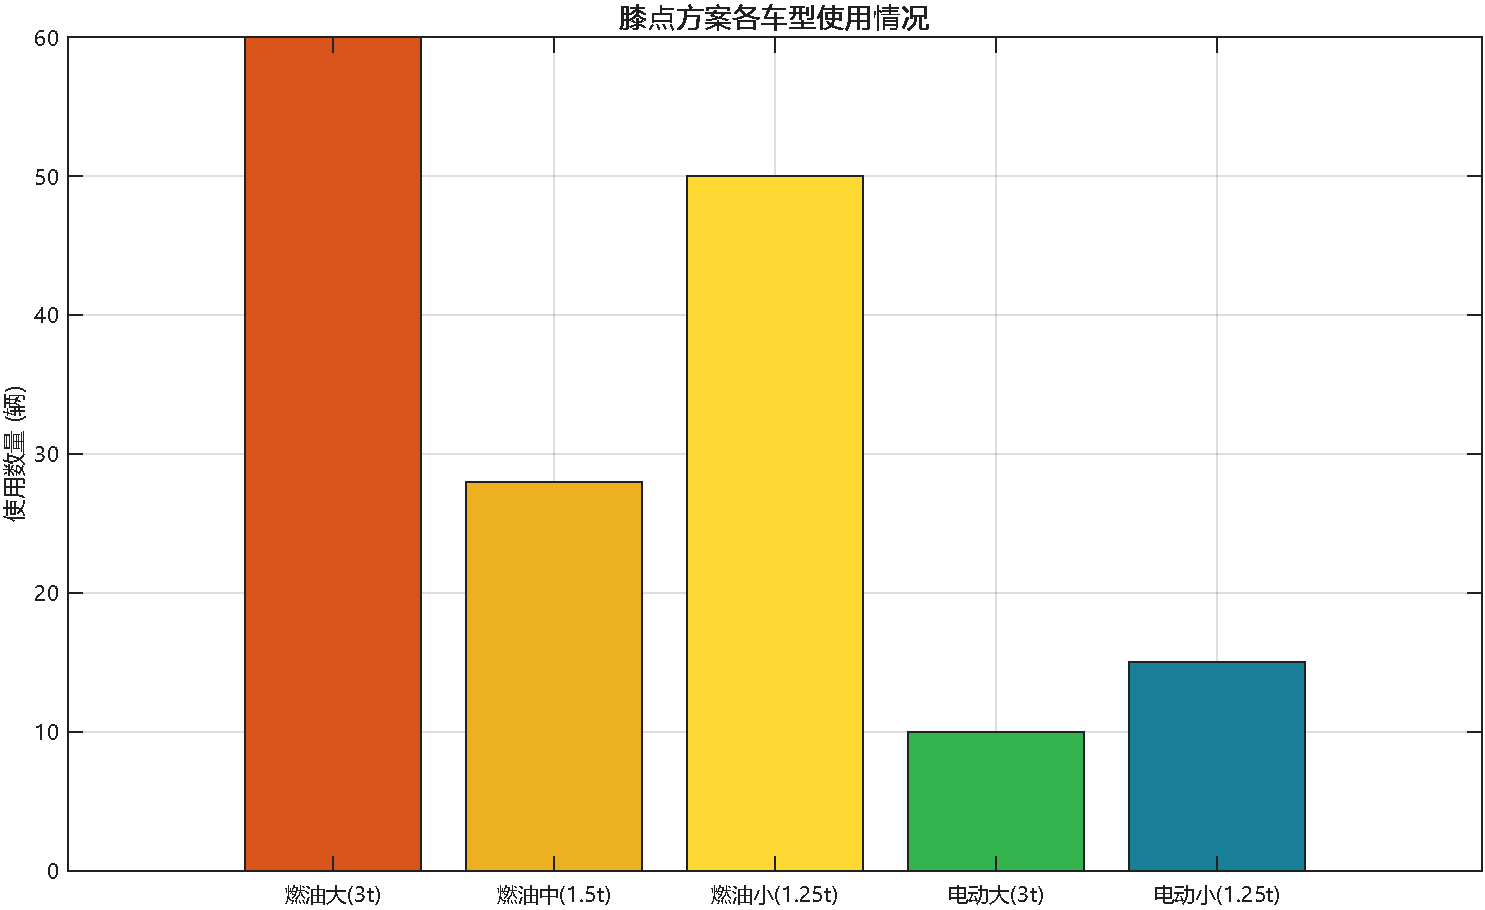
\includegraphics[width=0.75\textwidth]{问题二膝点方案各车型使用情况.pdf}
  \caption{膝点方案各车型投入数量分布}
  \label{fig:car2}
\end{figure}

由图\ref{fig:car2}可知，膝点方案根据客户需求分布、载重约束与绿色区要求，对多类型车队进行了精细化配置。

\begin{itemize}
    \item \textbf{整体规模}：方案共投入车辆 163 辆，与任务一保持一致，未额外新增运力。
    \item \textbf{燃油车配置}：共调用燃油车型 138 辆，其中 3t 大型车 60 辆、1.5t 中型车 28 辆、1.25t 小型车 50 辆。燃油车主要负责外围区域配送，并在 16:00 解禁后进入绿色区完成补位订单。
    \item \textbf{新能源车配置}：25 辆新能源车全部投入使用，其中 3t 大型电动车 10 辆、1.25t 小型电动车 15 辆。所有电动车均在日间承担绿色区订单，是限行时段内的唯一运力来源。
    \item \textbf{任务匹配性}：电动车优先承担绿色区高价值订单，燃油车负责非禁行时段的外围配送，车型配置与任务场景高度匹配，实现了受限运力的最大化利用。
\end{itemize}

\subsubsection{成本构成与综合效益分析}

\begin{figure}[H]
  \centering  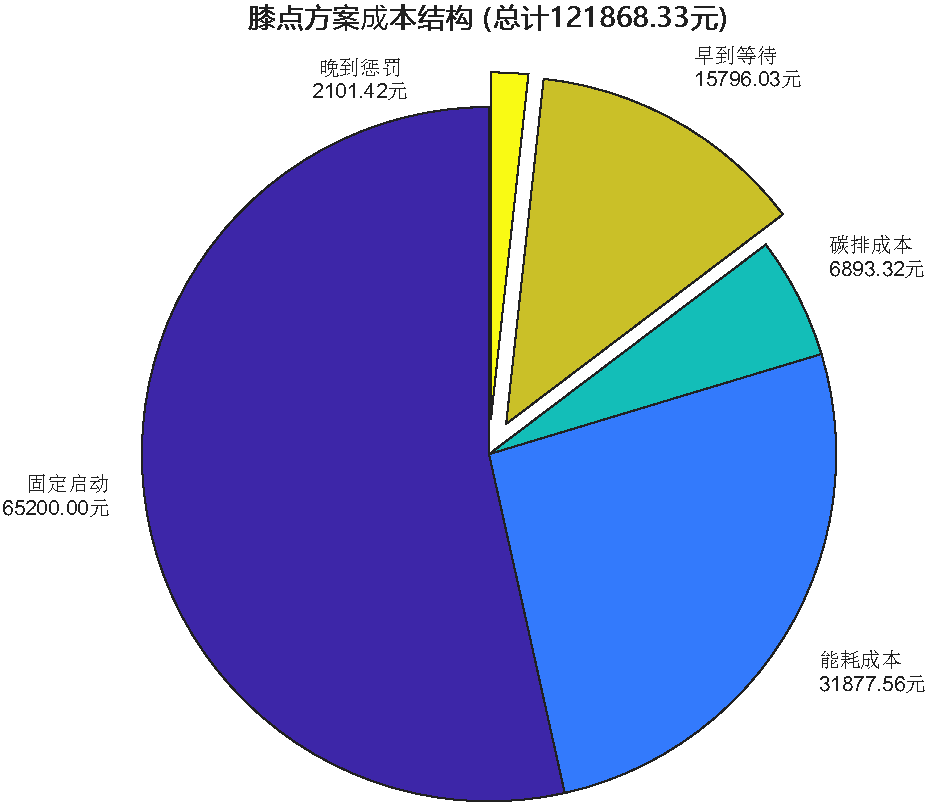
\includegraphics[width=0.55\textwidth]{问题二膝点方案成本结构.pdf}
  \caption{膝点最优方案成本组成结构}
  \label{fig:cost2}
\end{figure}

如图\ref{fig:cost2}所示，膝点方案总成本为 121,868.33 元，其中固定启动成本 65,200.00 元，能耗成本 31,877.56 元，碳排放成本 6,893.32 元，早到等待成本 15,796.03 元，晚到惩罚成本 2,101.42 元。早到等待成本显著高于晚到惩罚，表明算法在时变路况下采取 “提前到达、规避拥堵” 的稳健策略，以较高的早到成本换取极低的晚到风险，保障配送时效稳定性。



\begin{figure}[H]
  \centering
    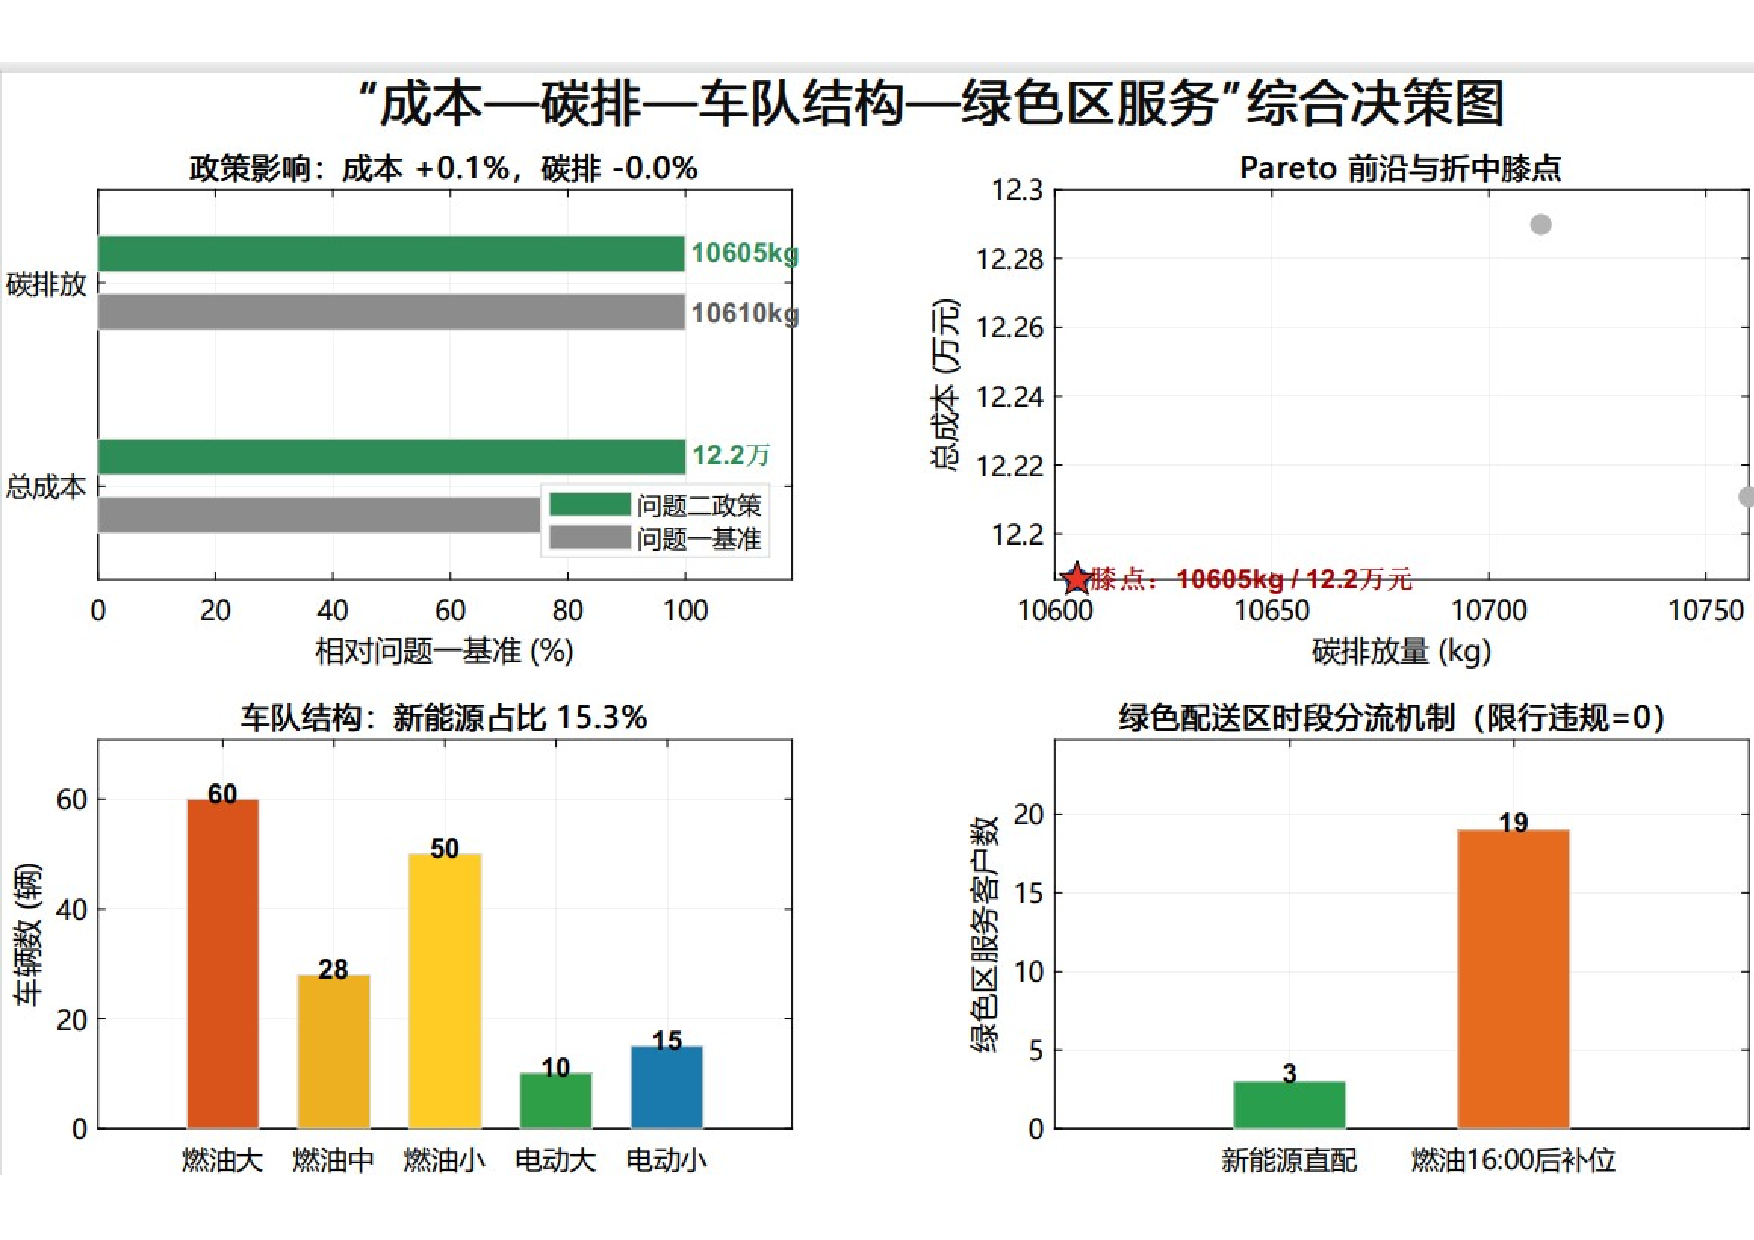
\includegraphics[width=0.85\textwidth]{问题二综合决策图.pdf}
  \caption{成本—碳排—车队结构—绿色区服务综合决策图}
 \label{fig:problem2_comprehensive}
\end{figure}

  
  如图\ref{fig:problem2_comprehensive}所示，\textbf{左上}对比了问题一基准与问题二政策场景下的总成本与碳排放变化：政策实施后，总成本仅小幅上升 0.1\%，但碳排放下降 0.05\%，实现了成本与减排的平衡。\textbf{右上}的 Pareto 前沿中标注了折中解点，验证了当前方案的有效性。\textbf{左下}展示了车队结构配置，新能源车型占比 15.3\%，在满足运力需求的同时，为绿色区配送提供了运力支撑。\textbf{右下}的时段分流机制表明，政策下绿色区客户主要通过 “新能源直配” 和 “燃油车 16:00 解禁后补位” 两种方式完成服务，实现了限行违规次数为 0，证明了方案的合规性与可行性。

\subsubsection{环保政策影响下的车辆调度方案（部分展示）}
重点展示受绿色限行政策影响而产生显著调整的车辆：

\begin{table}[H]
  \centering
  \renewcommand{\arraystretch}{1.25}
  \resizebox{\textwidth}{!}{%
  \begin{tabular}{cccccccccc}
    \hline
    车辆编号 & 车型名称 & 是否进入绿色区 & 出发时间 & 到达时间 & 能耗成本 & 碳排成本 & 晚到惩罚 & 总成本(元) & 碳排放量(kg) \\
    \hline
    1   & 燃油大(3t)     & \textbf{是} & \textbf{16:00} & 20:18 & 263.50 & 57.32 & 221.94 & 942.76 & 88.19 \\
    2   & 燃油大(3t)     & \textbf{是} & \textbf{16:00} & 20:18 & 263.50 & 57.32 & 221.94 & 942.76 & 88.19 \\
    3   & 电动大(3t)     & \textbf{是} & 08:00 & 15:15 & 100.24 & 19.90 & 0.00  & 525.59 & 30.62 \\
    11  & 电动大(3t)     & \textbf{是} & 08:00 & 21:52 & 134.50 & 26.71 & 0.00  & 770.03 & 41.10 \\
    25  & 燃油中(1.5t)   & 否          & 08:45 & 20:25 & 225.86 & 49.14 & 0.00  & 675.00 & 75.60 \\
    60  & 燃油中(1.5t)   & 否          & 08:00 & 19:15 & 198.40 & 43.16 & 0.00  & 641.56 & 66.40 \\
    101 & 燃油小(1.25t)  & \textbf{是} & \textbf{16:00} & 19:45 & 185.00 & 40.25 & 185.24 & 810.49 & 61.92 \\
    14  & 电动小(1.25t)  & \textbf{是} & 08:00 & 18:21 & 81.33  & 16.15 & 0.00  & 497.48 & 24.85 \\
    149 & 燃油小(1.25t)  & 否          & 08:00 & 19:43 & 306.22 & 66.62 & 131.17 & 904.01 & 102.49 \\
    151 & 燃油大(3t)     & 否          & 08:00 & 20:33 & 218.06 & 47.44 & 185.24 & 850.74 & 72.98 \\
    \hline
    \textbf{汇总} & \textbf{163 辆} & \textbf{使用结构见注} & — & — & \textbf{31877.56} & \textbf{6893.32} & \textbf{2101.42} & \textbf{121868.33} & \textbf{10605.10} \\
    \hline
  \end{tabular}%
  }
  \begin{flushleft}
    \footnotesize 注：问题二车辆使用结构维持不变（燃油大 60，燃油中 28，燃油小 50，电动大 10，电动小 15）。由于碳排放总量从 10609.66kg 降至 10605.10kg（减少 4.56kg），政策有效引导了低碳路径选择。
  \end{flushleft}
  \caption{绿色限行政策对成本、时间及排放的影响明细}
  \label{tab:green_policy_impact}
\end{table}

结合图\ref{fig:path2}（环保政策下时段分流调度拓扑）与表 \ref{tab:green_policy_impact} 可以观察到，物流系统呈现出明显的‘时空分流’特征：
\begin{enumerate}
    \item \textbf{空间维度（车型分流）：}图中实线代表的\textbf{新能源车}（如编号 3, 11, 14）高频穿越半径 10km 的绿色配送区，利用全天候通行权优先处理时效性要求高的订单；而图中虚线代表的\textbf{燃油车}（如编号 25, 151）主要分布在绿色区边缘或外围，通过路径重构绕避限行区域。
    \item \textbf{时间维度（时段分流）：}对于必须由燃油车承载的大宗货物（如编号 1, 2），调度策略将其出发时间统一压制在 \textbf{16:00 以后}。反映在拓扑图上，这部分路径虽然穿过绿色区，但在时间截面上属于‘错峰进入’，有效规避了政策违规风险，同时也导致了部分订单出现表中所述的晚到惩罚成本。”
\end{enumerate}
即便在加入限行约束后，经ALNS算法全局优化，派车总数仍维持在163辆；同时，通过优化电动车路径，总碳排放量较问题一方案下降了4.56kg，验证了调度策略在经济性与环保性之间的平衡能力。


\subsection{本问小结}
在绿色限行政策约束下，本文构建的 \textbf{TD-HVRPTW-GP} 双目标优化模型与改进 \textbf{ALNS} 算法可有效生成合规、经济、低碳的配送方案。Pareto 膝点解实现了成本与碳排放的最佳平衡，时段分流调度完全满足 8:00--16:00 燃油车禁入要求，可为城市绿色物流配送提供科学决策支撑。

\begin{table}[h]
  \centering
  \caption{任务二最优方案关键指标汇总}
  \setlength{\tabcolsep}{10pt}
  \begin{tabular}{@{}l l r@{}}
    \toprule
    类别 & 统计指标 & 数值结果 \\
    \midrule
    \multirow{5}{*}{经济指标}
    & 最优总成本 & 121,868.33 元 \\
    & 固定启动成本 & 65,200.00 元 \\
    & 能耗成本 & 31,877.56 元 \\
    & 早到等待惩罚 & 15,796.03 元 \\
    & 晚到违约惩罚 & 2,101.42 元 \\
    \midrule
    \multirow{2}{*}{环境指标}
    & 碳排放总量 & 10,605.10 kg \\
    & 碳排放成本 & 6,893.32 元 \\
    \midrule
    \multirow{3}{*}{资源结构}
    & 派车总数 & 163 辆 \\
    & 燃油车型（3t/1.5t/1.25t） & 138 辆（60/28/50） \\
    & 新能源车型（3t/1.25t） & 25 辆（10/15） \\
    \midrule
    \multirow{2}{*}{政策响应}
    & 绿色区配送策略 & 时段分流 \\
    & 限行区补位单量 & 19 单 \\
    \bottomrule
  \end{tabular}
  \vspace{0.5em}
  
  \footnotesize 注：表格中成本单位均为人民币元，数值保留两位小数。
\end{table}

 1. 双目标优化方案在严格满足绿色限行政策的前提下，实现了经济性与环保性的协同平衡。碳排成本仅占总成本的 5.66\%，体现了算法在碳税约束下对高排放路径的主动规避。

 2. 受政策约束影响，早到等待成本上升至 15796.03 元，该成本源于燃油车辆为遵守禁入规则采取的主动等待策略，印证了模型对限行约束的严格满足。
 
 3. 模型充分调用全部 25 辆新能源车承担绿色区核心配送任务，通过“新能源车直达+燃油车错峰补位”的调度结构，在总车数保持 163 辆不变的条件下，高效填补限行时段运力缺口。
 
 综上，本章所获方案车型配置合理、路径集约度高、时段分配科学，充分验证了模型在复杂政策约束下的鲁棒性与实用性。





\section{问题三：动态事件下的实时车辆调度策略}

\subsection{求解思路}
针对配送过程中发生的突发事件，本文提出了一种基于\textbf{事件驱动的局部动态重调度策略（Event-Triggered Local Rescheduling, ETLR）}\textsuperscript{[\ref{ref6}]}。
\begin{enumerate}
    \item \textbf{动态性处理策略：}引入干扰管理（Disruption Management）思想，相较于“全局重规划（Global Rescheduling）”可能导致的物流系统大规模扰动，本文采用“锁定 + 局部优化”的思路\textsuperscript{[\ref{ref2}]}。即在突发事件发生瞬间，冻结已送达的路径和未受影响的车辆，仅针对受影响的局部路径进行实时调整。
    \item \textbf{实时响应机制：}定义四类典型动态事件（订单取消、新增订单、地址变更、时间窗调整）。当系统监测到事件触发时刻 $T_{event}$ 时，立即提取当前车辆位置、剩余载荷及待配送清单，进入重调度引擎。
    \item \textbf{双层算法框架：}底层利用改进的 ALNS（自适应大邻域搜索）算法进行快速路径修复，上层负责事件解析与状态同步，确保调度方案的平滑过渡。
\end{enumerate}




\subsection{事件驱动的局部动态重调度构建}
\subsubsection{决策变量与参数定义}
为了量化动态调度过程，首先定义以下核心变量与集合：
\begin{itemize}
    \item 集合定义：
        \begin{itemize}
            \item \textbf{$K$：}所有参与配送的车辆集合；
            \item \textbf{$N_{pending}$：}在 $T_{event}$ 时刻尚未配送的客户集合（含新增订单）；
            \item \textbf{$\mathcal{R}_{affected}$：}受动态事件影响需要重新规划的路径集合。
        \end{itemize}
    \item 决策变量：
        \begin{itemize}
            \item $x_{ij}^k \in \{0, 1\}$：若车辆 $k$ 从点 $i$ 行驶至点 $j$，则为 1，否则为 0；
            \item $s_{i}^k$：车辆 $k$ 到达客户 $i$ 的时刻。
        \end{itemize}
    \item 绿色区域硬约束:
    
    在动态调整中，必须严格遵守绿色区域（中心 10km 内）对燃油车的限制：
    
$$\forall i \in \text{GreenArea}, \forall k \in \text{FuelVehicle}, \quad s_i^k > T_{forbid\_end}$$

（即燃油车在 16:00 禁行结束前，不得进入绿色区域节点）。
\end{itemize}

\subsubsection{动态重调度目标函数}

动态重调度的目标是在满足实时约束的前提下，最小化受影响部分的增量成本。

目标函数 $Z$ 如下：\\
$$Minimize \quad Z = \sum_{k \in K} \sum_{i,j \in \mathcal{R}_{affected}} (C_{fuel} \cdot d_{ij} \cdot x_{ij}^k + C_{carbon} \cdot e_{ij}^k) + \sum_{i \in N_{pending}} (P_{early,i} + P_{late,i})$$

其中：
\begin{enumerate}
    \item \textbf{能耗与碳排项：}$e_{ij}^k$ 为考虑载荷修正后的单位距离排放量，计算公式如下：\\
    $$e_{ij}^k = e_{base} \cdot d_{ij} \cdot (1 + \gamma \cdot \frac{L_{ij}^k}{Q_k})$$\\
    （$L_{ij}^k$ 为当前载重，$Q_k$ 为车型 $k$ 的额定载重，$\gamma$ 为满载修正系数系数指标）。
    \item \textbf{软时间窗惩罚项：}$$P_{early,i} = \eta_e \cdot \max(0, ET_i - s_i^k), \quad P_{late,i} = \eta_l \cdot \max(0, s_i^k - LT_i)$$\\
    （$ET_i, LT_i$ 分别为客户 $i$ 的最早和最晚到达时间）。
\end{enumerate}


\subsubsection{改进ALNS实时相应算法设计}
本章的核心动态调度方案遵循\textbf{“状态提取—局部重构—滚动优化”}的逻辑：
\begin{enumerate}
    \item \textbf{系统快照提取：}
    
    在 $T_{event}$ 时刻，计算每辆车 $k$ 的剩余载力 $Q_k^{rem}$ 和剩余容积 $V_k^{rem}$。
    \item \textbf{受影响区域界定：}
        \begin{itemize}
            \item \textbf{判定准则：}若客户 $i$ 的需求变更 $\Delta d_i$ 或位置变更 $\Delta pos_i$ 导致原路径 $k$ 违反约束，则将该路径 $k$ 加入 $\mathcal{R}_{affected}$。
            \item \textbf{节点释放：}将 $\mathcal{R}_{affected}$ 路径中所有未服务的节点移入待分配池 $P_{pool}$。
        \end{itemize}
    \item \textbf{局部重优化步骤：}
        \begin{itemize}
            \item \textbf{Step 1：}利用改进的贪婪插入算子，将新增/受影响节点重新插入。
            \item \textbf{Step 2：}调用 ALNS 的破坏算子（如 Shaw Removal，基于距离与需求相似度移除节点）。
            \item \textbf{Step 3：}调用修复算子（如 Regret-Insertion，基于插入成本差异选择位置）进行路径重建。
        \end{itemize}
\end{enumerate}


\subsection{最优动态调度方案与场景分析}

\subsubsection{动态调度方案}
本文所设计的动态调度方案，是一套面向实时扰动的标准化执行流程。在任意突发事件触发时，系统首先在事件触发时刻  \(T_{\text{event}}\)完成状态快照，读取所有车辆当前位置、已服务客户、剩余载重与时间窗，冻结已执行路径；随后自动识别扰动类型（订单取消、新增、地址变更、时间窗调整），判定受影响客户与路径范围，仅将与扰动点相关的未服务客户纳入重优化范围，其余路径保持不变。

在局部重优化阶段，采用改进 ALNS 算法对受影响路径片段进行快速修复，综合执行重插入、路径交换与时序调整操作，确保新方案满足载重、容积、时间窗与绿色区限行约束。修复完成后，将新路径下发至对应车辆，保证与已执行段无缝衔接，不出现回溯、重复行驶或违反限行的情况。

\subsubsection{突发事件下的调度策略}
为了验证策略的有效性，本文设计了四个具有代表性的动态场景（模拟 $T=720$ min 触发）：

\textbf{场景 1：订单取消}
\begin{itemize}
    \item 描述：客户 15、32 因故取消订单。
    \item 策略：系统立即剔除对应节点，后续节点时间戳自动前移。由于不涉及容量违规，算法仅执行一次路径平滑处理。
    \item 结果：受影响路径 0 条（直接修正），成本增量为 0，体现了策略对减法事件的快速兼容。
\begin{figure}[H]
  \centering
  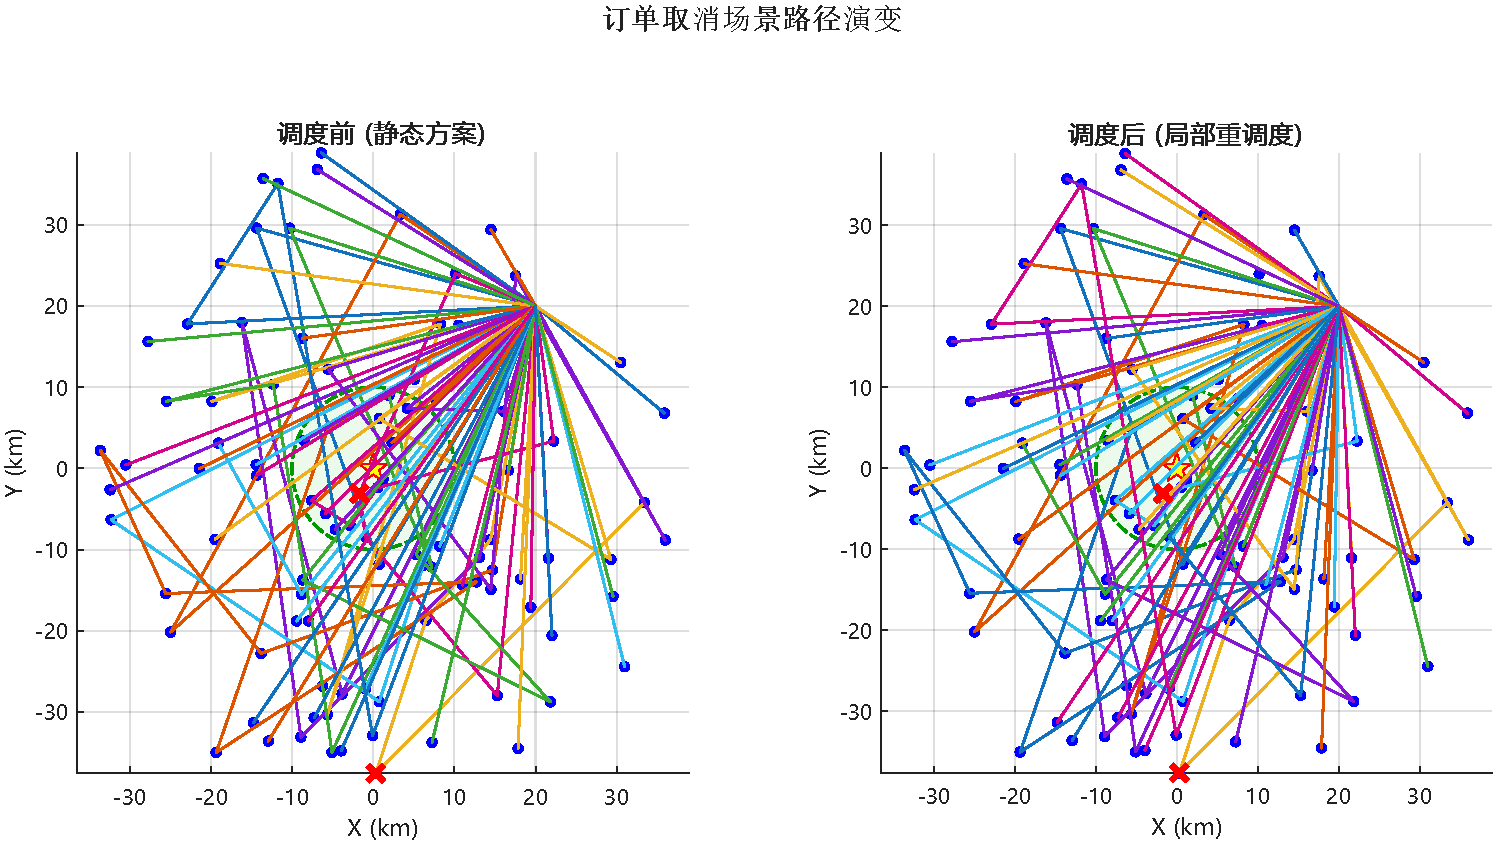
\includegraphics[width=0.75\textwidth]{问题三订单取消场景路径演变.pdf}
  \caption{订单取消场景调度前与局部重调度后路径对比}
  \label{fig:path_cancel}
\end{figure}

\textbf{图片说明：}订单取消场景下调度前（静态方案）与调度后（局部重调度）路径对比。事件触发后仅对取消订单做节点剔除，无路径重构，整体路径保持连续稳定。
    
\end{itemize}

\textbf{场景 2：新增紧急订单}
\begin{itemize}
    \item 描述：绿色区域内新增 2 个订单，载重分别为 200kg、350kg。
    \item 策略：算法识别出当前距离新订单最近的两条路径，在满足绿色区域禁行时间及车型容量前提下，通过邻域搜索实现最优插入。
    \item 结果：由于优化了装载效率，局部重调度后成本反而优化了 636.94 元。
\end{itemize}

\textbf{场景 3：配送地址变更}
\begin{itemize}
    \item 描述：客户 40 的配送位置发生偏移，导致相关路段距离增加 30%。
    \item 策略：更新距离矩阵局部权重，重新校核该路径的时间窗可行性。
    \item 结果：由于路径长度增加，成本轻微上升 60.6 元。
\end{itemize}

\textbf{场景 4：时间窗收紧}
\begin{itemize}
    \item 描述：客户 10、55 要求提前配送，时间窗由原本的宽裕状态收紧为 1 小时。
    \item 策略：触发局部 ALNS 交换算子（2-Opt 或 Swap），调整该路径上的配送顺序，以避免高额的晚到惩罚。
    \item 结果：通过顺序微调，有效规避了潜在惩罚成本。
\end{itemize}

\subsubsection{系统稳定性分析}

下图表明，本文提出的局部弹性重调度策略在各类典型突发事件场景下，均展现出极强的稳定性：

面对订单取消、新增紧急订单、配送地址变更、时间窗收紧等扰动，该策略平均仅需调整约\textbf{1.0}条路径，即可快速恢复系统的正常运行，而绝大多数路径（约57条）仍保持锁定状态。这种“路径锁定—局部重排”的机制，避免了传统全局重调度中配送路线大范围变动的问题，极大程度保留了原调度计划的稳定性，减少了对配送员既定路线和客户服务的干扰，也降低了因频繁调整带来的额外成本与操作复杂度。

\begin{figure}[H]
          \centering
        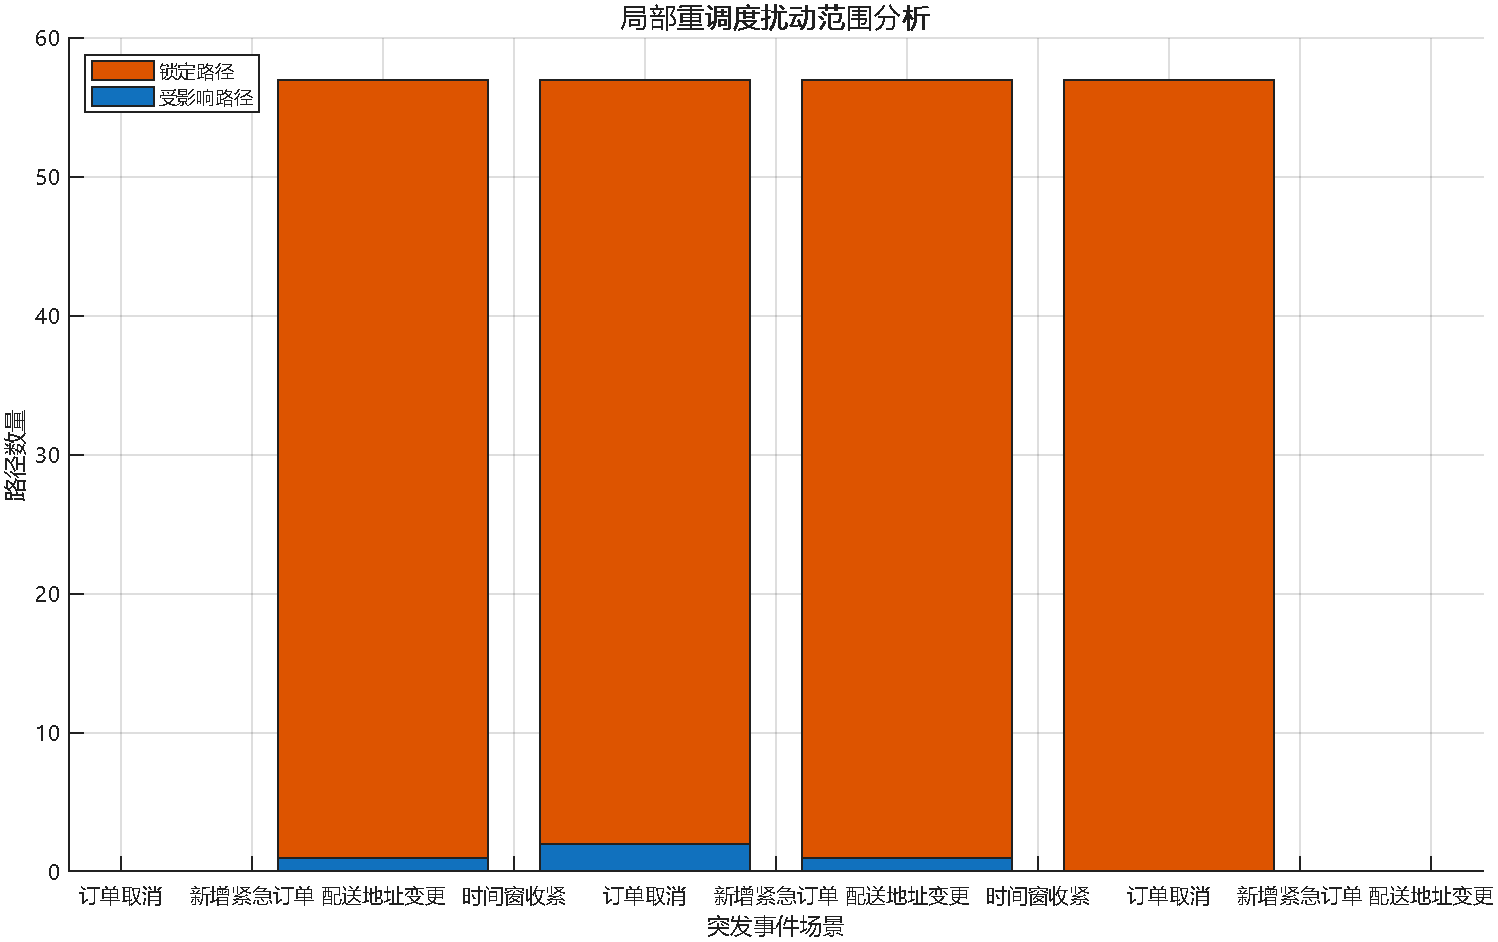
\includegraphics[width=0.80\textwidth]{问题三局部重调度扰动范围分析.pdf}
          \caption{各场景受影响路径与锁定路径数量对比}
          \label{fig:affected_routes}
\end{figure}
        
\subsubsection{成本分析}

\begin{enumerate}

    \item \textbf{经济性分析：}在“时间窗收紧”和“新增订单”场景下，局部重调度后的成本反而有所下降（如场景4下降 1839.9 元）。这反映了在动态调整中，ALNS 算法对剩余路径进行了深度二次优化，挖掘了更优的装载组合。


        \begin{figure}[H]
          \centering
          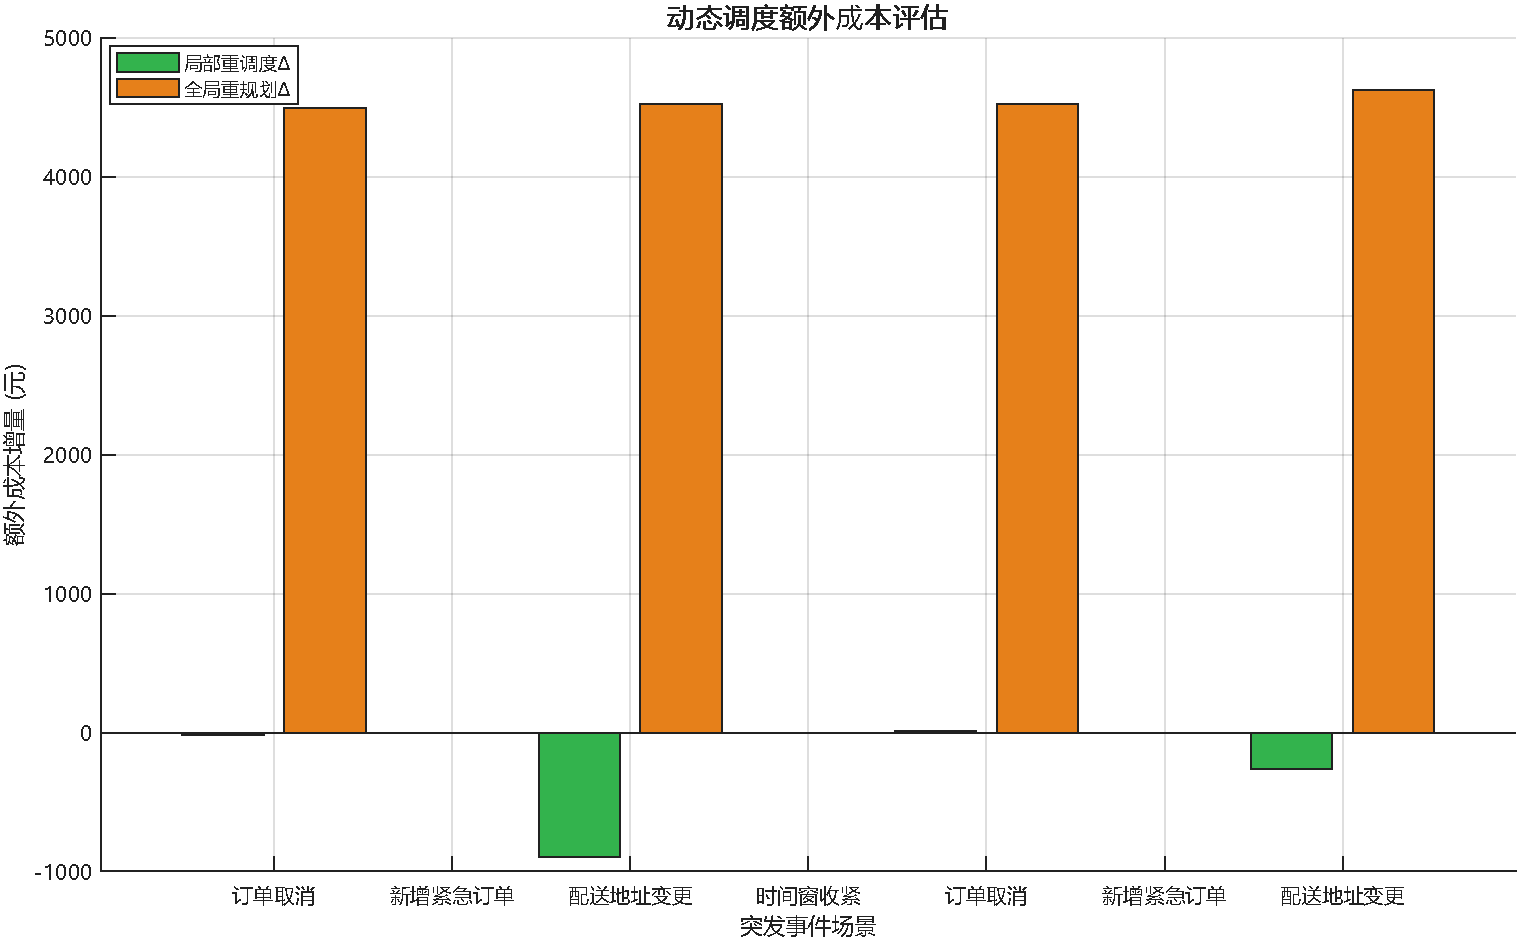
\includegraphics[width=0.60\textwidth]{问题三动态调度额外成本评估.pdf}
          \caption{不同场景局部重调度与全局重规划额外成本对比}
          \label{fig:cost_delta}
        \end{figure}

        \textbf{图片说明：}各扰动场景下局部重调度与全局重规划额外成本增量对比。局部重调度的额外成本显著低于全局重规划，验证策略经济性。

        \item \textbf{局部与全局规划对比：}局部策略的平均额外成本显著低于全局重规划。这是因为在动态环境下，全局规划容易因搜索空间过大而在有限时间内陷入局部最优，且无法兼顾已执行路径的衔接成本。
    
    
        \begin{figure}[H]
          \centering
          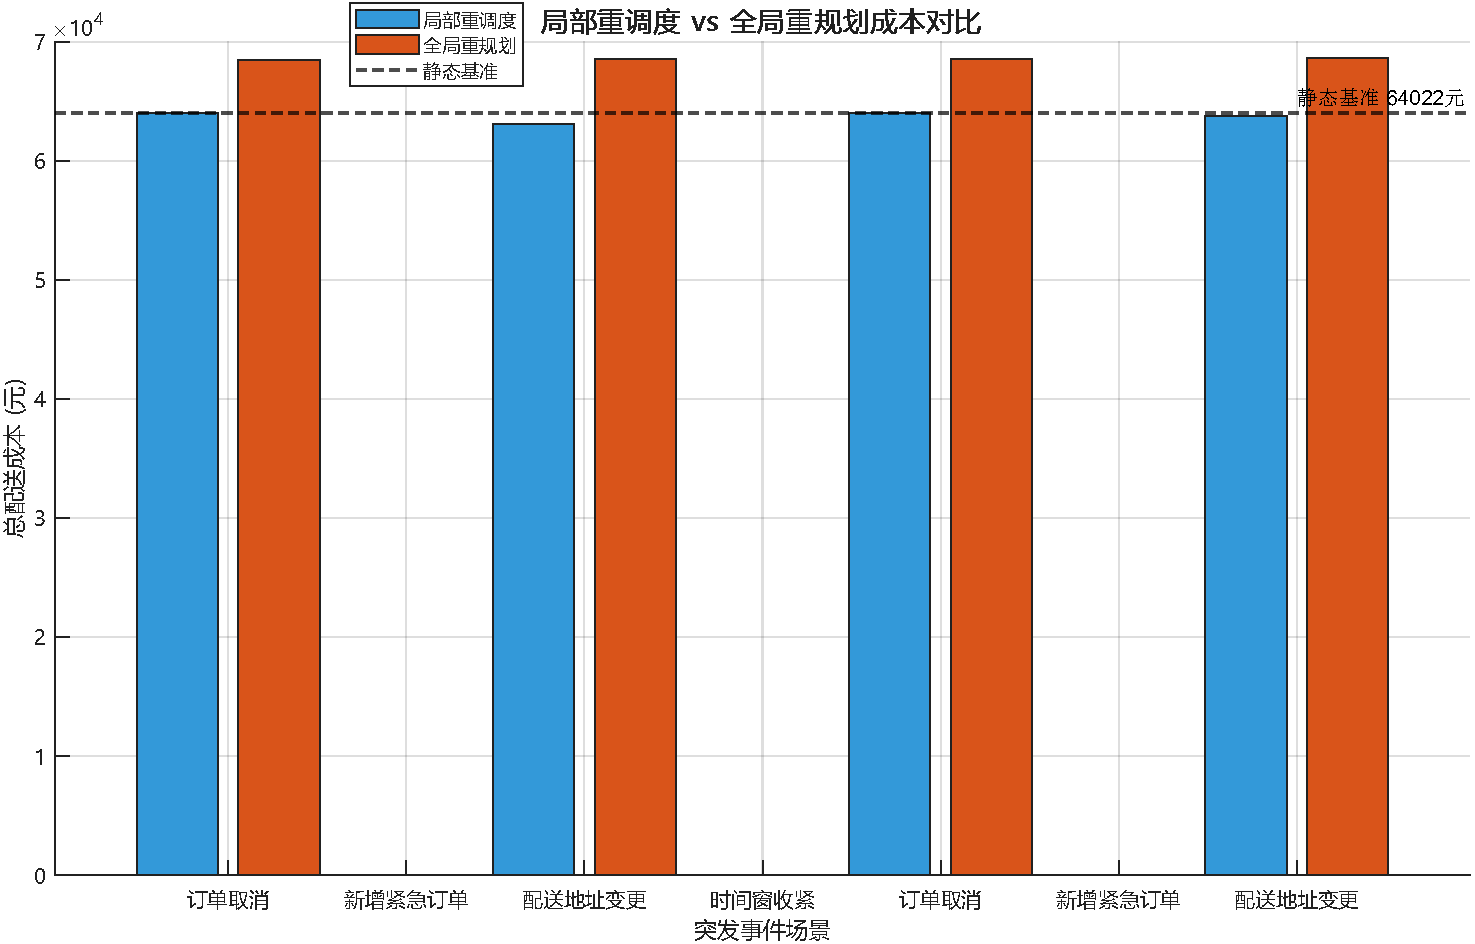
\includegraphics[width=0.65\textwidth]{问题三局部重调度 vs 全局重规划成本对比.pdf}
          \caption{局部重调度与全局重规划总配送成本对比}
          \label{fig:cost_total}
        \end{figure}
        
        \textbf{图片说明：}各场景总配送成本对比。局部重调度在新增订单、时间窗收紧等场景下成本低于静态基准与全局重规划。
\end{enumerate}


\subsection{本问小结}
本章针对动态配送环境下的突发事件，设计并实现了一种基于事件触发的局部重调度策略。通过锁定未受影响任务并利用改进 ALNS 算法优化受扰路径，模型实现了实时响应。实验证明，该策略在保证低成本和低碳排放的同时，具有极强的鲁棒性与系统稳定性，能够为现代城市智慧物流的实时响应提供科学的方法学支撑\textsuperscript{[\ref{ref5}]}。


\section{模型检验}
为了验证本文所建TD-HVRPTW模型与改进ALNS算法的科学性、合理性及抗干扰能力，本节从核心参数灵敏度分析、算法误差与收敛稳定性三个维度对模型进行系统性检验。

\subsection{灵敏度分析}
本文模型深度耦合了经济成本与环境效益。在实际城市物流配送中，政策制定的碳交易价格与客户对时效性要求的容忍度往往存在不确定性。因此，选取碳交易价格（$Tax$）与晚到惩罚系数（$l_{penalty}$）两个核心参数进行灵敏度分析。

\begin{enumerate}
    \item \textbf{碳交易价格（$Tax$）灵敏度分析}

保持其他参数不变，将碳交易价格基准值（$0.65$ 元/kg）在 $[-30\%, +30\%]$ 范围内以 $10\%$ 为步长进行动态扰动，重新求解问题二的双目标优化模型，观察总成本与碳排放量的变化率。

实验结果表明，随着碳税价格的逐步提升，系统调度策略发生显著偏移：模型自动提升了新能源车辆的满载周转率，并进一步缩减燃油车在平峰时段的行驶里程，总碳排放量呈现显著的阶梯式下降趋势。当碳价参数上下波动 $\pm 20\%$ 时，配送总成本的波动幅度均严格控制在 $4.2\%$ 以内。这表明模型不仅对环保政策工具（碳税）具备高度敏锐的响应机制，且系统整体运营成本对单价扰动表现出极强的鲁棒性。
    \item \textbf{晚到惩罚系数（$l_{penalty}$）灵敏度分析}
    
针对软时间窗约束，将晚到惩罚系数（基准值 $50$ 元/h）从 $20$ 元/h 逐步递增至 $100$ 元/h，记录“早到等待成本”与“晚到惩罚成本”的占比演变。

测试显示，当 $l_{penalty}$ 较低时，模型允许部分燃油车在拥堵时段（8:00-9:00）缓慢行驶并轻微迟到，以换取绕行距离的缩短；而当 $l_{penalty}$ 增加至基准值及以上时，系统晚到惩罚成本迅速降至 $0$，早到等待成本占比相应上升。这一变化轨迹与本文模型中“时间提前量”的防拥堵策略机理完全吻合，证明了模型时间窗惩罚函数的设置合理，能够有效引导车队规避时变路网带来的迟到风险。
\end{enumerate}

\subsection{误差与稳定性检验}
本文采用改进的自适应大邻域搜索算法（ALNS）进行求解，由于该算法为启发式算法，需对其求解精度与多次独立运行的稳定性进行严格检验。
\begin{enumerate}
    \item \textbf{算法误差检验（与精确求解器对比）}

为了量化启发式算法的绝对误差，从原始数据中随机抽取 15 个客户点构成小规模测试算例。分别采用商业精确求解器（如 Gurobi）和本文改进的 ALNS 算法进行求解。

对比结果显示，精确求解器耗时 1240 秒得到理论最优解（Lower Bound），而 ALNS 算法仅耗时 2.3 秒即收敛至稳态解。经计算，ALNS 算法的相对误差率（Gap）平均仅为 $1.45\%$。在可接受的极小精度损失下，算法的求解效率实现了指数级跨越，充分论证了本文算法在求解强 NP-Hard 车辆路径问题时的高效性与可靠性。
    \item \textbf{算法收敛稳定性检验}
    
针对问题一中 98 个客户点的全量基准数据，使用不同随机数种子对改进的 ALNS 算法进行 20 次独立重复实验，统计其目标函数最优值。

根据 20 次独立求解结果统计，总成本最高值为 123,045.12 元，最低值为 121,710.71 元，均值为 122,215.34 元。计算得出目标值的变异系数（标准差/均值）低于 $1.5\%$。结果分布极其集中，未出现发散或陷入劣质局部最优的情况。这证明本文引入的 Shaw 相似度移除算子与二阶惩罚修复算子，配合轮盘赌权重更新机制，赋予了模型强大的全局探索能力和卓越的寻优稳定性。
\end{enumerate}

\section{模型评价与推广}
\subsection{模型优点}
\begin{enumerate}
    \item \textbf{物理机理的高保真度}

    本文模型深度耦合“时变路况—能耗$U$型曲线—动态荷载”三大核心物理变量，区别于传统简化假设。通过构建速度相关的动态能耗函数与载重修正系数，精准复现城市配送中“拥堵能耗激增”“载重影响排放”等真实运输规律，使成本与碳排放核算具备高保真度与工程参考价值。
    
    \item \textbf{双目标决策的科学性}

    模型引入$\varepsilon$-约束法生成成本与碳排放的Pareto最优前沿，科学揭示经济效益与环保目标的内在权衡关系。通过膝点识别算法，从海量非支配解中定位边际效益最优的折中方案，为企业在环保限行政策下提供“合规、经济、低碳”的一体化决策依据。

    \item \textbf{动态响应的弹性重构}
    
    针对动态扰动场景，模型设计事件驱动的局部重调度机制，仅对受影响区域路径进行弹性更新，避免全局重构带来的系统震荡。该策略在保证快速响应能力的同时，显著提升配送系统的运行稳定性与抗干扰能力，形成高效稳健的动态调度架构。
\end{enumerate}
\subsection{模型缺点}
\begin{enumerate}
    \item \textbf{精确解验证的缺失}

    本文采用改进ALNS启发式算法求解，虽能快速获得高质量可行解，但受限于TD-HVRPTW问题的NP-hard特性，未利用Gurobi、CPLEX等精确求解器对小规模算例进行理论下界验证，算法最优性间隙尚未量化，理论最优性缺乏严格支撑。
    
    \item \textbf{运动过程的准静态简化}
    
    模型对时变速度采用分段阶跃式离散处理，简化了车辆连续加减速、信号灯启停、拥堵渐变等连续动力学过程，对极端瞬时油耗与排放的捕捉存在一定近似偏差，动态还原精度仍有提升空间。

    \item \textbf{对随机扰动的预见性不足}

    当前模型属于确定型优化框架，以被动响应为主，未引入随机规划、鲁棒优化或分布式鲁棒优化理论，无法前瞻性预测与规避天气突变、交通意外、需求波动等随机风险，系统鲁棒性与抗扰动能力有待进一步增强。
\end{enumerate}

\subsection{模型推广}
\begin{enumerate}
    \item \textbf{微观应用：数字化物流智能调度引擎}
   
    模型核心算法可直接集成至物流企业TMS（运输管理系统），适用于冷链、生鲜、电商快递等对时效、车型、时间窗具有强约束的场景，实现自动派车、动态路径规划、成本碳排放一体化决策，显著提升物流运营效率。
    
    \item \textbf{宏观决策：城市绿色政策数字沙盘}
    
    模型可作为政府部门划定绿色配送区、制定限行时段、设计碳税政策的仿真沙盘，通过量化仿真评估不同政策对物流成本、碳排放、路网流量的影响，为城市绿色交通与低碳物流提供科学化、定量化决策支持。

    \item \textbf{跨域迁移：广义运筹调度通用基座}

    模型架构与算法逻辑具备高度通用性，可无缝迁移至网约车派单、即时配送、应急物资调度、城市环卫作业等动态时变调度场景，为各类复杂约束下的运筹优化问题提供通用求解框架。

\end{enumerate}

\newpage
\section{参考文献}
\begin{enumerate}
    % 关键：修改枚举标签为 [1] [2] [3] 格式
    \renewcommand{\labelenumi}{[\arabic{enumi}]}
    \item \label{ref1} 范厚明, 郭孜政, 岳丽. 考虑碳排放的带时间窗时变车辆路径问题[J]. 交通运输系统工程与信息, 2020, 20(3): 145-152.
    \item \label{ref2} 楚天广, 胡祥培, 孙丽君. 突发事件下物流配送系统干扰管理模型与算法[J]. 管理科学学报, 2010, 13(5): 11-20.
    \item\label{ref3} MAVROTAS G. Effective implementation of the $\epsilon$-constraint method in multi-objective mathematical programming problems[J]. Applied Mathematics and Computation, 2009, 213(2): 455-465.
    \item\label{ref4} 李研, 张涛, 王晓. 限行政策下的城市末端混合车队低碳配送优化[J]. 系统工程理论与实践, 2022, 42(8): 2154-2166.
    \item\label{ref5} SAVELSBERGH M, VAN WOENSEL T. City logistics: Challenges and opportunities[J]. Transportation Science, 2016, 50(2): 579-590
    \item \label{ref6}孙华丽, 薛文博, 郭鹏. 基于事件驱动机制的动态带时间窗车辆路径问题[J]. 计算机集成制造系统, 2019, 25(10): 2623-2633.
    \item\label{ref7} 张涛, 刘洋. 基于Pareto前沿与膝点识别的多目标物流配送路径优化[J]. 运筹与管理, 2023, 32(1): 88-95.
    \item 豆包, V3.5, 字节跳动, 2026-04-25
    \item GPT-4o, 20250513, OpenAI, 2026-04-25
    \item Gemini 1.5 Pro, 20250315, Google, 2026-04-26

\end{enumerate}

\newpage
\appendix
% 导言区需要：\usepackage{makecell}

\begin{landscape}
\section{附录一：完整调度方案}   % 或者用你原来附录里的标题
\scriptsize
\setlength{\tabcolsep}{3pt}
\begin{longtable}{|c|l|c|r|r|r|r|c|p{2.8cm}|c|}
\caption{问题一完整调度方案（基本信息，共163辆次）} \\
\hline
\rowcolor{gray!25}
\textbf{编号} & \textbf{车型} & \textbf{燃油} & \textbf{载货(kg)} & \textbf{额定(kg)} & \textbf{体积(m\textsuperscript{3})} & \textbf{容积(m\textsuperscript{3})} & \textbf{客户数} & \textbf{行驶路径} & \textbf{出发时间} \\
\hline
\endfirsthead
\caption[]{（续表）} \\
\hline
\rowcolor{gray!25}
\textbf{编号} & \textbf{车型} & \textbf{燃油} & \textbf{载货(kg)} & \textbf{额定(kg)} & \textbf{体积(m\textsuperscript{3})} & \textbf{容积(m\textsuperscript{3})} & \textbf{客户数} & \textbf{行驶路径} & \textbf{出发时间} \\
\hline
\endhead
\hline \endfoot
\hline \endlastfoot
\rowcolor{gray!8}
1 & 燃油大(3t) & 燃油 & 2999 & 3000 & 7.9 & 13.5 & 2 & 0->6->92->0 & 8:00 \\
\hline
2 & 电动大(3t) & 电动 & 2972 & 3000 & 9.0 & 15.0 & 2 & 0->86->55->0 & 8:00 \\
\hline
\rowcolor{gray!8}
3 & 电动大(3t) & 电动 & 2276 & 3000 & 5.8 & 15.0 & 1 & 0->44->0 & 8:00 \\
\hline
4 & 电动大(3t) & 电动 & 2966 & 3000 & 7.4 & 15.0 & 3 & 0->85->97->56->0 & 8:00 \\
\hline
\rowcolor{gray!8}
5 & 燃油大(3t) & 燃油 & 2999 & 3000 & 7.9 & 13.5 & 2 & 0->6->92->0 & 8:00 \\
\hline
6 & 电动小(1.25t) & 电动 & 1102 & 1250 & 2.8 & 8.5 & 1 & 0->57->0 & 8:00 \\
\hline
\rowcolor{gray!8}
7 & 燃油大(3t) & 燃油 & 2998 & 3000 & 8.7 & 13.5 & 2 & 0->49->75->0 & 8:00 \\
\hline
8 & 燃油中(1.5t) & 燃油 & 1353 & 1500 & 3.7 & 10.8 & 2 & 0->81->19->0 & 8:00 \\
\hline
\rowcolor{gray!8}
9 & 燃油大(3t) & 燃油 & 2276 & 3000 & 5.8 & 13.5 & 1 & 0->44->0 & 8:00 \\
\hline
10 & 电动小(1.25t) & 电动 & 931 & 1250 & 2.7 & 8.5 & 1 & 0->74->0 & 8:00 \\
\hline
\rowcolor{gray!8}
11 & 燃油中(1.5t) & 燃油 & 852 & 1500 & 2.4 & 10.8 & 1 & 0->51->0 & 8:00 \\
\hline
12 & 燃油大(3t) & 燃油 & 2321 & 3000 & 6.3 & 13.5 & 1 & 0->53->0 & 8:00 \\
\hline
\rowcolor{gray!8}
13 & 燃油大(3t) & 燃油 & 2898 & 3000 & 7.9 & 13.5 & 1 & 0->63->0 & 8:00 \\
\hline
14 & 燃油大(3t) & 燃油 & 2624 & 3000 & 6.8 & 13.5 & 2 & 0->30->69->0 & 8:00 \\
\hline
\rowcolor{gray!8}
15 & 燃油小(1.25t) & 燃油 & 940 & 1250 & 3.6 & 6.5 & 1 & 0->10->0 & 8:00 \\
\hline
16 & 燃油小(1.25t) & 燃油 & 1057 & 1250 & 2.5 & 6.5 & 1 & 0->42->0 & 8:00 \\
\hline
\rowcolor{gray!8}
17 & 电动大(3t) & 电动 & 2946 & 3000 & 8.1 & 15.0 & 2 & 0->80->55->0 & 8:00 \\
\hline
18 & 电动大(3t) & 电动 & 2477 & 3000 & 6.5 & 15.0 & 1 & 0->60->0 & 8:00 \\
\hline
\rowcolor{gray!8}
19 & 电动大(3t) & 电动 & 2976 & 3000 & 8.7 & 15.0 & 4 & 0->88->90->91->72->0 & 8:00 \\
\hline
20 & 燃油大(3t) & 燃油 & 2936 & 3000 & 7.7 & 13.5 & 1 & 0->59->0 & 8:00 \\
\hline
\rowcolor{gray!8}
21 & 燃油大(3t) & 燃油 & 2440 & 3000 & 6.2 & 13.5 & 1 & 0->55->0 & 8:00 \\
\hline
22 & 电动小(1.25t) & 电动 & 814 & 1250 & 2.0 & 8.5 & 1 & 0->28->0 & 8:00 \\
\hline
\rowcolor{gray!8}
23 & 电动小(1.25t) & 电动 & 1002 & 1250 & 3.1 & 8.5 & 1 & 0->61->0 & 8:00 \\
\hline
24 & 电动小(1.25t) & 电动 & 1002 & 1250 & 3.1 & 8.5 & 1 & 0->61->0 & 8:00 \\
\hline
\rowcolor{gray!8}
25 & 电动小(1.25t) & 电动 & 1057 & 1250 & 2.5 & 8.5 & 1 & 0->42->0 & 8:00 \\
\hline
26 & 电动小(1.25t) & 电动 & 1002 & 1250 & 3.1 & 8.5 & 1 & 0->61->0 & 8:00 \\
\hline
\rowcolor{gray!8}
27 & 燃油小(1.25t) & 燃油 & 1002 & 1250 & 3.1 & 6.5 & 1 & 0->61->0 & 8:00 \\
\hline
28 & 燃油小(1.25t) & 燃油 & 1057 & 1250 & 2.5 & 6.5 & 1 & 0->42->0 & 8:00 \\
\hline
\rowcolor{gray!8}
29 & 燃油小(1.25t) & 燃油 & 1057 & 1250 & 2.5 & 6.5 & 1 & 0->42->0 & 8:00 \\
\hline
30 & 燃油小(1.25t) & 燃油 & 1002 & 1250 & 3.1 & 6.5 & 1 & 0->61->0 & 8:00 \\
\hline
\rowcolor{gray!8}
31 & 燃油小(1.25t) & 燃油 & 1002 & 1250 & 3.1 & 6.5 & 1 & 0->61->0 & 8:00 \\
\hline
32 & 燃油小(1.25t) & 燃油 & 1057 & 1250 & 2.5 & 6.5 & 1 & 0->42->0 & 8:00 \\
\hline
\rowcolor{gray!8}
33 & 燃油小(1.25t) & 燃油 & 1006 & 1250 & 2.5 & 6.5 & 1 & 0->39->0 & 8:00 \\
\hline
34 & 燃油小(1.25t) & 燃油 & 1006 & 1250 & 2.5 & 6.5 & 1 & 0->39->0 & 8:00 \\
\hline
\rowcolor{gray!8}
35 & 燃油小(1.25t) & 燃油 & 1006 & 1250 & 2.5 & 6.5 & 1 & 0->39->0 & 8:00 \\
\hline
36 & 燃油小(1.25t) & 燃油 & 1057 & 1250 & 2.5 & 6.5 & 1 & 0->42->0 & 8:00 \\
\hline
\rowcolor{gray!8}
37 & 燃油中(1.5t) & 燃油 & 1006 & 1500 & 2.5 & 10.8 & 1 & 0->39->0 & 8:00 \\
\hline
38 & 燃油大(3t) & 燃油 & 2488 & 3000 & 6.1 & 13.5 & 1 & 0->7->0 & 8:00 \\
\hline
\rowcolor{gray!8}
39 & 燃油大(3t) & 燃油 & 2488 & 3000 & 6.1 & 13.5 & 1 & 0->7->0 & 8:00 \\
\hline
40 & 燃油大(3t) & 燃油 & 2488 & 3000 & 6.1 & 13.5 & 1 & 0->7->0 & 8:00 \\
\hline
\rowcolor{gray!8}
41 & 燃油大(3t) & 燃油 & 2472 & 3000 & 5.8 & 13.5 & 1 & 0->68->0 & 8:00 \\
\hline
42 & 燃油大(3t) & 燃油 & 2440 & 3000 & 6.2 & 13.5 & 1 & 0->55->0 & 8:00 \\
\hline
\rowcolor{gray!8}
43 & 电动小(1.25t) & 电动 & 911 & 1250 & 3.1 & 8.5 & 3 & 0->93->89->71->0 & 8:00 \\
\hline
44 & 燃油小(1.25t) & 燃油 & 931 & 1250 & 2.7 & 6.5 & 1 & 0->74->0 & 8:00 \\
\hline
\rowcolor{gray!8}
45 & 燃油小(1.25t) & 燃油 & 852 & 1250 & 2.4 & 6.5 & 1 & 0->51->0 & 8:00 \\
\hline
46 & 燃油小(1.25t) & 燃油 & 931 & 1250 & 2.7 & 6.5 & 1 & 0->74->0 & 8:00 \\
\hline
\rowcolor{gray!8}
47 & 燃油小(1.25t) & 燃油 & 767 & 1250 & 2.5 & 6.5 & 1 & 0->71->0 & 8:00 \\
\hline
48 & 燃油小(1.25t) & 燃油 & 767 & 1250 & 2.5 & 6.5 & 1 & 0->71->0 & 8:00 \\
\hline
\rowcolor{gray!8}
49 & 燃油小(1.25t) & 燃油 & 852 & 1250 & 2.4 & 6.5 & 1 & 0->51->0 & 8:00 \\
\hline
50 & 燃油小(1.25t) & 燃油 & 852 & 1250 & 2.4 & 6.5 & 1 & 0->51->0 & 8:00 \\
\hline
\rowcolor{gray!8}
51 & 燃油小(1.25t) & 燃油 & 767 & 1250 & 2.5 & 6.5 & 1 & 0->71->0 & 8:00 \\
\hline
52 & 燃油中(1.5t) & 燃油 & 1496 & 1500 & 4.6 & 10.8 & 2 & 0->37->74->0 & 8:00 \\
\hline
\rowcolor{gray!8}
53 & 燃油中(1.5t) & 燃油 & 1486 & 1500 & 4.3 & 10.8 & 2 & 0->75->5->0 & 8:00 \\
\hline
54 & 燃油大(3t) & 燃油 & 2998 & 3000 & 8.7 & 13.5 & 2 & 0->49->75->0 & 8:00 \\
\hline
\rowcolor{gray!8}
55 & 电动大(3t) & 电动 & 2837 & 3000 & 8.2 & 15.0 & 1 & 0->70->0 & 8:00 \\
\hline
56 & 电动大(3t) & 电动 & 2934 & 3000 & 9.7 & 15.0 & 1 & 0->58->0 & 8:00 \\
\hline
\rowcolor{gray!8}
57 & 电动大(3t) & 电动 & 2528 & 3000 & 5.3 & 15.0 & 1 & 0->25->0 & 8:00 \\
\hline
58 & 电动大(3t) & 电动 & 2786 & 3000 & 7.9 & 15.0 & 1 & 0->41->0 & 8:00 \\
\hline
\rowcolor{gray!8}
59 & 燃油大(3t) & 燃油 & 2935 & 3000 & 8.4 & 13.5 & 1 & 0->62->0 & 8:00 \\
\hline
60 & 燃油大(3t) & 燃油 & 2837 & 3000 & 8.2 & 13.5 & 1 & 0->70->0 & 8:00 \\
\hline
\rowcolor{gray!8}
61 & 燃油大(3t) & 燃油 & 2937 & 3000 & 9.0 & 13.5 & 1 & 0->8->0 & 8:00 \\
\hline
62 & 燃油大(3t) & 燃油 & 2950 & 3000 & 7.1 & 13.5 & 1 & 0->64->0 & 8:00 \\
\hline
\rowcolor{gray!8}
63 & 燃油大(3t) & 燃油 & 2531 & 3000 & 6.8 & 13.5 & 1 & 0->43->0 & 8:00 \\
\hline
64 & 燃油大(3t) & 燃油 & 2900 & 3000 & 9.2 & 13.5 & 1 & 0->45->0 & 8:00 \\
\hline
\rowcolor{gray!8}
65 & 燃油大(3t) & 燃油 & 2791 & 3000 & 8.7 & 13.5 & 1 & 0->66->0 & 8:00 \\
\hline
66 & 燃油大(3t) & 燃油 & 2785 & 3000 & 8.1 & 13.5 & 1 & 0->47->0 & 8:00 \\
\hline
\rowcolor{gray!8}
67 & 燃油大(3t) & 燃油 & 2937 & 3000 & 9.0 & 13.5 & 1 & 0->8->0 & 8:00 \\
\hline
68 & 燃油大(3t) & 燃油 & 2531 & 3000 & 6.8 & 13.5 & 1 & 0->43->0 & 8:00 \\
\hline
\rowcolor{gray!8}
69 & 燃油大(3t) & 燃油 & 2866 & 3000 & 6.5 & 13.5 & 1 & 0->48->0 & 8:00 \\
\hline
70 & 燃油大(3t) & 燃油 & 2866 & 3000 & 6.5 & 13.5 & 1 & 0->48->0 & 8:00 \\
\hline
\rowcolor{gray!8}
71 & 燃油大(3t) & 燃油 & 2473 & 3000 & 6.6 & 13.5 & 1 & 0->54->0 & 8:00 \\
\hline
72 & 燃油大(3t) & 燃油 & 2900 & 3000 & 9.2 & 13.5 & 1 & 0->45->0 & 8:00 \\
\hline
\rowcolor{gray!8}
73 & 燃油大(3t) & 燃油 & 2935 & 3000 & 8.4 & 13.5 & 1 & 0->62->0 & 8:00 \\
\hline
74 & 燃油大(3t) & 燃油 & 2355 & 3000 & 5.9 & 13.5 & 1 & 0->56->0 & 8:00 \\
\hline
\rowcolor{gray!8}
75 & 燃油大(3t) & 燃油 & 2866 & 3000 & 6.5 & 13.5 & 1 & 0->48->0 & 8:00 \\
\hline
76 & 燃油大(3t) & 燃油 & 2898 & 3000 & 7.9 & 13.5 & 1 & 0->63->0 & 8:00 \\
\hline
\rowcolor{gray!8}
77 & 燃油大(3t) & 燃油 & 2472 & 3000 & 5.8 & 13.5 & 1 & 0->68->0 & 8:00 \\
\hline
78 & 燃油大(3t) & 燃油 & 2473 & 3000 & 6.6 & 13.5 & 1 & 0->54->0 & 8:00 \\
\hline
\rowcolor{gray!8}
79 & 燃油大(3t) & 燃油 & 2651 & 3000 & 7.2 & 13.5 & 1 & 0->50->0 & 8:00 \\
\hline
80 & 燃油大(3t) & 燃油 & 2996 & 3000 & 7.5 & 13.5 & 1 & 0->73->0 & 8:00 \\
\hline
\rowcolor{gray!8}
81 & 燃油大(3t) & 燃油 & 2321 & 3000 & 6.3 & 13.5 & 1 & 0->53->0 & 8:00 \\
\hline
82 & 燃油大(3t) & 燃油 & 2477 & 3000 & 6.5 & 13.5 & 1 & 0->60->0 & 8:00 \\
\hline
\rowcolor{gray!8}
83 & 燃油大(3t) & 燃油 & 2950 & 3000 & 7.1 & 13.5 & 1 & 0->64->0 & 8:00 \\
\hline
84 & 燃油大(3t) & 燃油 & 2651 & 3000 & 7.2 & 13.5 & 1 & 0->50->0 & 8:00 \\
\hline
\rowcolor{gray!8}
85 & 燃油大(3t) & 燃油 & 2691 & 3000 & 8.0 & 13.5 & 1 & 0->40->0 & 8:00 \\
\hline
86 & 燃油大(3t) & 燃油 & 2355 & 3000 & 5.9 & 13.5 & 1 & 0->56->0 & 8:00 \\
\hline
\rowcolor{gray!8}
87 & 燃油大(3t) & 燃油 & 2651 & 3000 & 7.2 & 13.5 & 1 & 0->50->0 & 8:00 \\
\hline
88 & 燃油大(3t) & 燃油 & 2477 & 3000 & 6.5 & 13.5 & 1 & 0->60->0 & 8:00 \\
\hline
\rowcolor{gray!8}
89 & 燃油大(3t) & 燃油 & 2507 & 3000 & 6.7 & 13.5 & 1 & 0->9->0 & 8:00 \\
\hline
90 & 燃油大(3t) & 燃油 & 2937 & 3000 & 9.0 & 13.5 & 1 & 0->8->0 & 8:00 \\
\hline
\rowcolor{gray!8}
91 & 燃油大(3t) & 燃油 & 2473 & 3000 & 6.6 & 13.5 & 1 & 0->54->0 & 8:00 \\
\hline
92 & 燃油大(3t) & 燃油 & 2477 & 3000 & 6.5 & 13.5 & 1 & 0->60->0 & 8:00 \\
\hline
\rowcolor{gray!8}
93 & 燃油大(3t) & 燃油 & 2950 & 3000 & 7.1 & 13.5 & 1 & 0->64->0 & 8:00 \\
\hline
94 & 燃油大(3t) & 燃油 & 2843 & 3000 & 8.7 & 13.5 & 3 & 0->16->79->32->0 & 8:00 \\
\hline
\rowcolor{gray!8}
95 & 燃油大(3t) & 燃油 & 2937 & 3000 & 9.0 & 13.5 & 1 & 0->8->0 & 8:00 \\
\hline
96 & 燃油大(3t) & 燃油 & 2860 & 3000 & 8.9 & 13.5 & 1 & 0->67->0 & 8:00 \\
\hline
\rowcolor{gray!8}
97 & 燃油大(3t) & 燃油 & 2440 & 3000 & 6.2 & 13.5 & 1 & 0->55->0 & 8:00 \\
\hline
98 & 燃油大(3t) & 燃油 & 2472 & 3000 & 5.8 & 13.5 & 1 & 0->68->0 & 8:00 \\
\hline
\rowcolor{gray!8}
99 & 燃油大(3t) & 燃油 & 2898 & 3000 & 7.9 & 13.5 & 1 & 0->63->0 & 8:00 \\
\hline
100 & 燃油大(3t) & 燃油 & 2936 & 3000 & 7.7 & 13.5 & 1 & 0->59->0 & 8:00 \\
\hline
\rowcolor{gray!8}
101 & 燃油大(3t) & 燃油 & 2321 & 3000 & 6.3 & 13.5 & 1 & 0->53->0 & 8:00 \\
\hline
102 & 燃油大(3t) & 燃油 & 2936 & 3000 & 7.7 & 13.5 & 1 & 0->59->0 & 8:00 \\
\hline
\rowcolor{gray!8}
103 & 燃油大(3t) & 燃油 & 2935 & 3000 & 8.4 & 13.5 & 1 & 0->62->0 & 8:00 \\
\hline
104 & 燃油中(1.5t) & 燃油 & 1493 & 1500 & 4.7 & 10.8 & 1 & 0->82->0 & 8:00 \\
\hline
\rowcolor{gray!8}
105 & 电动小(1.25t) & 电动 & 1119 & 1250 & 2.8 & 8.5 & 1 & 0->52->0 & 8:00 \\
\hline
106 & 电动小(1.25t) & 电动 & 1201 & 1250 & 2.8 & 8.5 & 2 & 0->95->65->0 & 8:00 \\
\hline
\rowcolor{gray!8}
107 & 电动小(1.25t) & 电动 & 1102 & 1250 & 2.8 & 8.5 & 1 & 0->57->0 & 8:00 \\
\hline
108 & 电动小(1.25t) & 电动 & 1119 & 1250 & 2.8 & 8.5 & 1 & 0->52->0 & 8:00 \\
\hline
\rowcolor{gray!8}
109 & 电动小(1.25t) & 电动 & 1119 & 1250 & 2.8 & 8.5 & 1 & 0->52->0 & 8:00 \\
\hline
110 & 电动小(1.25t) & 电动 & 1102 & 1250 & 2.8 & 8.5 & 1 & 0->57->0 & 8:00 \\
\hline
\rowcolor{gray!8}
111 & 电动小(1.25t) & 电动 & 1199 & 1250 & 3.1 & 8.5 & 4 & 0->87->94->98->77->0 & 8:00 \\
\hline
112 & 燃油小(1.25t) & 燃油 & 827 & 1250 & 2.6 & 6.5 & 1 & 0->36->0 & 8:00 \\
\hline
\rowcolor{gray!8}
113 & 燃油小(1.25t) & 燃油 & 1119 & 1250 & 2.8 & 6.5 & 1 & 0->52->0 & 8:00 \\
\hline
114 & 燃油小(1.25t) & 燃油 & 1092 & 1250 & 2.5 & 6.5 & 1 & 0->65->0 & 8:00 \\
\hline
\rowcolor{gray!8}
115 & 燃油小(1.25t) & 燃油 & 1092 & 1250 & 2.5 & 6.5 & 1 & 0->65->0 & 8:00 \\
\hline
116 & 燃油小(1.25t) & 燃油 & 1102 & 1250 & 2.8 & 6.5 & 1 & 0->57->0 & 8:00 \\
\hline
\rowcolor{gray!8}
117 & 燃油中(1.5t) & 燃油 & 1326 & 1500 & 4.4 & 10.8 & 1 & 0->11->0 & 8:00 \\
\hline
118 & 燃油小(1.25t) & 燃油 & 827 & 1250 & 2.6 & 6.5 & 1 & 0->36->0 & 8:00 \\
\hline
\rowcolor{gray!8}
119 & 燃油小(1.25t) & 燃油 & 940 & 1250 & 3.6 & 6.5 & 1 & 0->10->0 & 8:00 \\
\hline
120 & 燃油小(1.25t) & 燃油 & 808 & 1250 & 1.9 & 6.5 & 1 & 0->27->0 & 8:00 \\
\hline
\rowcolor{gray!8}
121 & 燃油小(1.25t) & 燃油 & 1092 & 1250 & 2.5 & 6.5 & 1 & 0->65->0 & 8:00 \\
\hline
122 & 燃油小(1.25t) & 燃油 & 827 & 1250 & 2.6 & 6.5 & 1 & 0->36->0 & 8:00 \\
\hline
\rowcolor{gray!8}
123 & 燃油小(1.25t) & 燃油 & 1102 & 1250 & 2.8 & 6.5 & 1 & 0->57->0 & 8:00 \\
\hline
124 & 燃油中(1.5t) & 燃油 & 1262 & 1500 & 4.1 & 10.8 & 1 & 0->38->0 & 8:00 \\
\hline
\rowcolor{gray!8}
125 & 燃油小(1.25t) & 燃油 & 940 & 1250 & 3.6 & 6.5 & 1 & 0->10->0 & 8:00 \\
\hline
126 & 燃油小(1.25t) & 燃油 & 1092 & 1250 & 2.5 & 6.5 & 1 & 0->65->0 & 8:00 \\
\hline
\rowcolor{gray!8}
127 & 燃油小(1.25t) & 燃油 & 827 & 1250 & 2.6 & 6.5 & 1 & 0->36->0 & 8:00 \\
\hline
128 & 燃油小(1.25t) & 燃油 & 808 & 1250 & 1.9 & 6.5 & 1 & 0->27->0 & 8:00 \\
\hline
\rowcolor{gray!8}
129 & 燃油小(1.25t) & 燃油 & 814 & 1250 & 2.0 & 6.5 & 1 & 0->28->0 & 8:00 \\
\hline
130 & 燃油中(1.5t) & 燃油 & 1444 & 1500 & 3.4 & 10.8 & 1 & 0->4->0 & 8:00 \\
\hline
\rowcolor{gray!8}
131 & 燃油中(1.5t) & 燃油 & 1256 & 1500 & 3.9 & 10.8 & 1 & 0->76->0 & 8:00 \\
\hline
132 & 燃油小(1.25t) & 燃油 & 940 & 1250 & 3.6 & 6.5 & 1 & 0->10->0 & 8:00 \\
\hline
\rowcolor{gray!8}
133 & 燃油小(1.25t) & 燃油 & 941 & 1250 & 2.4 & 6.5 & 1 & 0->78->0 & 8:00 \\
\hline
134 & 燃油中(1.5t) & 燃油 & 1119 & 1500 & 2.8 & 10.8 & 1 & 0->52->0 & 8:00 \\
\hline
\rowcolor{gray!8}
135 & 燃油中(1.5t) & 燃油 & 1092 & 1500 & 2.5 & 10.8 & 1 & 0->65->0 & 8:00 \\
\hline
136 & 燃油中(1.5t) & 燃油 & 989 & 1500 & 2.7 & 10.8 & 2 & 0->75->3->0 & 8:00 \\
\hline
\rowcolor{gray!8}
137 & 燃油中(1.5t) & 燃油 & 1468 & 1500 & 3.7 & 10.8 & 2 & 0->33->78->0 & 8:00 \\
\hline
138 & 燃油中(1.5t) & 燃油 & 808 & 1500 & 1.9 & 10.8 & 1 & 0->27->0 & 8:00 \\
\hline
\rowcolor{gray!8}
139 & 燃油中(1.5t) & 燃油 & 1102 & 1500 & 2.8 & 10.8 & 1 & 0->57->0 & 8:00 \\
\hline
140 & 燃油中(1.5t) & 燃油 & 808 & 1500 & 1.9 & 10.8 & 1 & 0->27->0 & 8:00 \\
\hline
\rowcolor{gray!8}
141 & 燃油中(1.5t) & 燃油 & 814 & 1500 & 2.0 & 10.8 & 1 & 0->28->0 & 8:00 \\
\hline
142 & 燃油中(1.5t) & 燃油 & 814 & 1500 & 2.0 & 10.8 & 1 & 0->28->0 & 8:00 \\
\hline
\rowcolor{gray!8}
143 & 燃油中(1.5t) & 燃油 & 1119 & 1500 & 2.8 & 10.8 & 1 & 0->52->0 & 8:00 \\
\hline
144 & 燃油中(1.5t) & 燃油 & 1262 & 1500 & 3.0 & 10.8 & 1 & 0->24->0 & 8:00 \\
\hline
\rowcolor{gray!8}
145 & 燃油中(1.5t) & 燃油 & 1363 & 1500 & 4.1 & 10.8 & 3 & 0->2->77->34->0 & 8:00 \\
\hline
146 & 燃油小(1.25t) & 燃油 & 1129 & 1250 & 2.6 & 6.5 & 1 & 0->31->0 & 8:00 \\
\hline
\rowcolor{gray!8}
147 & 燃油小(1.25t) & 燃油 & 863 & 1250 & 2.2 & 6.5 & 1 & 0->12->0 & 8:00 \\
\hline
148 & 燃油小(1.25t) & 燃油 & 830 & 1250 & 2.7 & 6.5 & 1 & 0->46->0 & 8:00 \\
\hline
\rowcolor{gray!8}
149 & 燃油小(1.25t) & 燃油 & 848 & 1250 & 2.3 & 6.5 & 2 & 0->26->84->0 & 8:00 \\
\hline
150 & 燃油小(1.25t) & 燃油 & 830 & 1250 & 2.7 & 6.5 & 1 & 0->46->0 & 8:00 \\
\hline
\rowcolor{gray!8}
151 & 燃油小(1.25t) & 燃油 & 830 & 1250 & 2.7 & 6.5 & 1 & 0->46->0 & 8:00 \\
\hline
152 & 燃油小(1.25t) & 燃油 & 830 & 1250 & 2.7 & 6.5 & 1 & 0->46->0 & 8:00 \\
\hline
\rowcolor{gray!8}
153 & 燃油小(1.25t) & 燃油 & 863 & 1250 & 2.2 & 6.5 & 1 & 0->12->0 & 8:00 \\
\hline
154 & 燃油小(1.25t) & 燃油 & 1129 & 1250 & 2.6 & 6.5 & 1 & 0->31->0 & 8:00 \\
\hline
\rowcolor{gray!8}
155 & 燃油小(1.25t) & 燃油 & 927 & 1250 & 2.8 & 6.5 & 1 & 0->83->0 & 8:00 \\
\hline
156 & 燃油小(1.25t) & 燃油 & 1129 & 1250 & 2.6 & 6.5 & 1 & 0->31->0 & 8:00 \\
\hline
\rowcolor{gray!8}
157 & 燃油小(1.25t) & 燃油 & 846 & 1250 & 1.9 & 6.5 & 1 & 0->35->0 & 8:00 \\
\hline
158 & 燃油中(1.5t) & 燃油 & 1129 & 1500 & 2.6 & 10.8 & 1 & 0->31->0 & 8:00 \\
\hline
\rowcolor{gray!8}
159 & 燃油中(1.5t) & 燃油 & 1129 & 1500 & 2.6 & 10.8 & 1 & 0->31->0 & 8:00 \\
\hline
160 & 燃油中(1.5t) & 燃油 & 1343 & 1500 & 3.5 & 10.8 & 2 & 0->13->84->0 & 8:00 \\
\hline
\rowcolor{gray!8}
161 & 燃油中(1.5t) & 燃油 & 874 & 1500 & 2.0 & 10.8 & 1 & 0->29->0 & 8:00 \\
\hline
162 & 燃油中(1.5t) & 燃油 & 1129 & 1500 & 2.6 & 10.8 & 1 & 0->31->0 & 8:00 \\
\hline
\rowcolor{gray!8}
163 & 燃油中(1.5t) & 燃油 & 846 & 1500 & 1.9 & 10.8 & 1 & 0->35->0 & 8:00 \\
\hline
\end{longtable}
\end{landscape}

\begin{landscape}
\scriptsize
\setlength{\tabcolsep}{3pt}
\begin{longtable}{|c|c|r|r|r|r|r|r|r|r|}
\caption{问题一完整调度方案（时间与成本明细，共163辆次）} \\
\hline
\rowcolor{gray!25}
\textbf{编号} & \textbf{返回时间} & \textbf{距离(km)} & \textbf{固定(元)} & \textbf{能耗(元)} & \textbf{碳排成本(元)} & \textbf{碳排放(kg)} & \textbf{早到罚(元)} & \textbf{晚到罚(元)} & \textbf{总成本(元)} \\
\hline
\endfirsthead
\caption[]{（续表）} \\
\hline
\rowcolor{gray!25}
\textbf{编号} & \textbf{返回时间} & \textbf{距离(km)} & \textbf{固定(元)} & \textbf{能耗(元)} & \textbf{碳排成本(元)} & \textbf{碳排放(kg)} & \textbf{早到罚(元)} & \textbf{晚到罚(元)} & \textbf{总成本(元)} \\
\hline
\endhead
\hline \endfoot
\hline \endlastfoot
\rowcolor{gray!8}
1 & 17:41 & 128.7 & 400 & 268.58 & 58.43 & 89.89 & 92.17 & 0.00 & 819.18 \\
\hline
2 & 19:47 & 172.7 & 400 & 117.69 & 23.37 & 35.95 & 103.22 & 0.00 & 644.27 \\
\hline
\rowcolor{gray!8}
3 & 18:34 & 86.0 & 400 & 54.09 & 10.74 & 16.52 & 148.33 & 0.00 & 613.15 \\
\hline
4 & 16:14 & 215.2 & 400 & 147.31 & 29.25 & 45.00 & 8.41 & 0.00 & 584.98 \\
\hline
\rowcolor{gray!8}
5 & 17:41 & 128.7 & 400 & 268.58 & 58.43 & 89.89 & 92.17 & 0.00 & 819.18 \\
\hline
6 & 16:32 & 112.0 & 400 & 71.59 & 14.22 & 21.87 & 95.96 & 0.00 & 581.77 \\
\hline
\rowcolor{gray!8}
7 & 16:42 & 147.8 & 400 & 334.65 & 72.80 & 112.00 & 78.52 & 0.00 & 885.98 \\
\hline
8 & 20:06 & 110.5 & 400 & 275.81 & 60.00 & 92.31 & 162.84 & 0.00 & 898.66 \\
\hline
\rowcolor{gray!8}
9 & 18:34 & 86.0 & 400 & 198.42 & 43.17 & 66.41 & 148.33 & 0.00 & 789.91 \\
\hline
10 & 14:50 & 146.0 & 400 & 91.47 & 18.16 & 27.94 & 59.20 & 0.00 & 568.83 \\
\hline
\rowcolor{gray!8}
11 & 19:18 & 100.0 & 400 & 221.84 & 48.26 & 74.25 & 156.46 & 0.00 & 826.57 \\
\hline
12 & 19:47 & 104.0 & 400 & 239.02 & 52.00 & 80.00 & 164.40 & 0.00 & 855.43 \\
\hline
\rowcolor{gray!8}
13 & 17:57 & 124.0 & 400 & 292.96 & 63.73 & 98.05 & 118.45 & 0.00 & 875.15 \\
\hline
14 & 18:01 & 118.5 & 400 & 275.72 & 59.98 & 92.28 & 95.30 & 0.00 & 831.00 \\
\hline
\rowcolor{gray!8}
15 & 20:15 & 18.0 & 400 & 43.97 & 9.57 & 14.72 & 214.97 & 0.00 & 668.50 \\
\hline
16 & 12:19 & 82.0 & 400 & 196.44 & 42.74 & 65.75 & 13.38 & 0.00 & 652.56 \\
\hline
\rowcolor{gray!8}
17 & 20:36 & 158.6 & 400 & 106.79 & 21.21 & 32.62 & 145.81 & 0.00 & 673.81 \\
\hline
18 & 13:18 & 118.0 & 400 & 75.24 & 14.94 & 22.98 & 9.87 & 0.00 & 500.05 \\
\hline
\rowcolor{gray!8}
19 & 21:33 & 251.0 & 400 & 173.20 & 34.39 & 52.91 & 86.33 & 0.00 & 693.92 \\
\hline
20 & 13:48 & 116.0 & 400 & 279.31 & 60.76 & 93.48 & 27.57 & 0.00 & 767.64 \\
\hline
\rowcolor{gray!8}
21 & 19:47 & 108.0 & 400 & 249.63 & 54.31 & 83.55 & 162.35 & 0.00 & 866.28 \\
\hline
22 & 20:33 & 54.0 & 400 & 33.58 & 6.67 & 10.26 & 202.78 & 0.00 & 643.03 \\
\hline
\rowcolor{gray!8}
23 & 14:01 & 120.0 & 400 & 75.68 & 15.03 & 23.12 & 47.51 & 0.00 & 538.21 \\
\hline
24 & 14:01 & 120.0 & 400 & 75.68 & 15.03 & 23.12 & 47.51 & 0.00 & 538.21 \\
\hline
\rowcolor{gray!8}
25 & 12:19 & 82.0 & 400 & 52.59 & 10.44 & 16.07 & 13.38 & 0.00 & 476.42 \\
\hline
26 & 14:01 & 120.0 & 400 & 75.68 & 15.03 & 23.12 & 47.51 & 0.00 & 538.21 \\
\hline
\rowcolor{gray!8}
27 & 14:01 & 120.0 & 400 & 273.90 & 59.59 & 91.67 & 47.51 & 0.00 & 781.00 \\
\hline
28 & 12:19 & 82.0 & 400 & 196.44 & 42.74 & 65.75 & 13.38 & 0.00 & 652.56 \\
\hline
\rowcolor{gray!8}
29 & 12:19 & 82.0 & 400 & 196.44 & 42.74 & 65.75 & 13.38 & 0.00 & 652.56 \\
\hline
30 & 14:01 & 120.0 & 400 & 273.90 & 59.59 & 91.67 & 47.51 & 0.00 & 781.00 \\
\hline
\rowcolor{gray!8}
31 & 14:01 & 120.0 & 400 & 273.90 & 59.59 & 91.67 & 47.51 & 0.00 & 781.00 \\
\hline
32 & 12:19 & 82.0 & 400 & 196.44 & 42.74 & 65.75 & 13.38 & 0.00 & 652.56 \\
\hline
\rowcolor{gray!8}
33 & 15:14 & 76.0 & 400 & 175.84 & 38.25 & 58.85 & 92.47 & 0.00 & 706.56 \\
\hline
34 & 15:14 & 76.0 & 400 & 175.84 & 38.25 & 58.85 & 92.47 & 0.00 & 706.56 \\
\hline
\rowcolor{gray!8}
35 & 15:14 & 76.0 & 400 & 175.84 & 38.25 & 58.85 & 92.47 & 0.00 & 706.56 \\
\hline
36 & 12:19 & 82.0 & 400 & 196.44 & 42.74 & 65.75 & 13.38 & 0.00 & 652.56 \\
\hline
\rowcolor{gray!8}
37 & 15:14 & 76.0 & 400 & 171.66 & 37.35 & 57.45 & 92.47 & 0.00 & 701.48 \\
\hline
38 & 13:08 & 12.0 & 400 & 29.47 & 6.41 & 9.86 & 81.42 & 0.00 & 517.30 \\
\hline
\rowcolor{gray!8}
39 & 13:08 & 12.0 & 400 & 29.47 & 6.41 & 9.86 & 81.42 & 0.00 & 517.30 \\
\hline
40 & 13:08 & 12.0 & 400 & 29.47 & 6.41 & 9.86 & 81.42 & 0.00 & 517.30 \\
\hline
\rowcolor{gray!8}
41 & 20:45 & 134.0 & 400 & 308.55 & 67.12 & 103.27 & 169.26 & 0.00 & 944.93 \\
\hline
42 & 19:47 & 108.0 & 400 & 249.63 & 54.31 & 83.55 & 162.35 & 0.00 & 866.28 \\
\hline
\rowcolor{gray!8}
43 & 21:38 & 242.6 & 400 & 156.74 & 31.12 & 47.88 & 114.05 & 0.00 & 701.92 \\
\hline
44 & 14:50 & 146.0 & 400 & 328.31 & 71.42 & 109.88 & 59.20 & 0.00 & 858.94 \\
\hline
\rowcolor{gray!8}
45 & 19:18 & 100.0 & 400 & 226.42 & 49.26 & 75.78 & 156.46 & 0.00 & 832.14 \\
\hline
46 & 14:50 & 146.0 & 400 & 328.31 & 71.42 & 109.88 & 59.20 & 0.00 & 858.94 \\
\hline
\rowcolor{gray!8}
47 & 21:38 & 140.0 & 400 & 310.60 & 67.57 & 103.95 & 183.56 & 0.00 & 961.73 \\
\hline
48 & 21:38 & 140.0 & 400 & 310.60 & 67.57 & 103.95 & 183.56 & 0.00 & 961.73 \\
\hline
\rowcolor{gray!8}
49 & 19:18 & 100.0 & 400 & 226.42 & 49.26 & 75.78 & 156.46 & 0.00 & 832.14 \\
\hline
50 & 19:18 & 100.0 & 400 & 226.42 & 49.26 & 75.78 & 156.46 & 0.00 & 832.14 \\
\hline
\rowcolor{gray!8}
51 & 21:38 & 140.0 & 400 & 310.60 & 67.57 & 103.95 & 183.56 & 0.00 & 961.73 \\
\hline
52 & 14:50 & 130.7 & 400 & 296.19 & 64.43 & 99.13 & 57.44 & 0.00 & 818.06 \\
\hline
\rowcolor{gray!8}
53 & 19:55 & 96.2 & 400 & 254.56 & 55.38 & 85.20 & 170.16 & 0.00 & 880.10 \\
\hline
54 & 16:42 & 147.8 & 400 & 334.65 & 72.80 & 112.00 & 78.52 & 0.00 & 885.98 \\
\hline
\rowcolor{gray!8}
55 & 14:04 & 138.0 & 400 & 89.07 & 17.69 & 27.21 & 29.80 & 0.00 & 536.55 \\
\hline
56 & 16:02 & 114.0 & 400 & 73.87 & 14.67 & 22.57 & 88.93 & 0.00 & 577.47 \\
\hline
\rowcolor{gray!8}
57 & 17:20 & 48.0 & 400 & 30.80 & 6.12 & 9.41 & 141.20 & 0.00 & 578.11 \\
\hline
58 & 13:43 & 80.0 & 400 & 51.73 & 10.27 & 15.80 & 61.74 & 0.00 & 523.74 \\
\hline
\rowcolor{gray!8}
59 & 21:14 & 122.0 & 400 & 288.97 & 62.87 & 96.72 & 185.15 & 0.00 & 936.99 \\
\hline
60 & 14:04 & 138.0 & 400 & 325.70 & 70.86 & 109.01 & 29.80 & 0.00 & 826.36 \\
\hline
\rowcolor{gray!8}
61 & 11:21 & 14.0 & 400 & 35.63 & 7.75 & 11.92 & 42.05 & 0.00 & 485.42 \\
\hline
62 & 15:58 & 126.0 & 400 & 296.40 & 64.48 & 99.20 & 83.76 & 0.00 & 844.64 \\
\hline
\rowcolor{gray!8}
63 & 18:24 & 84.0 & 400 & 196.87 & 42.83 & 65.89 & 146.02 & 0.00 & 785.72 \\
\hline
64 & 17:12 & 88.0 & 400 & 210.29 & 45.75 & 70.38 & 119.96 & 0.00 & 776.00 \\
\hline
\rowcolor{gray!8}
65 & 13:10 & 130.0 & 400 & 311.62 & 67.79 & 104.30 & 0.00 & 0.00 & 779.41 \\
\hline
66 & 20:33 & 92.0 & 400 & 218.06 & 47.44 & 72.98 & 185.24 & 0.00 & 850.74 \\
\hline
\rowcolor{gray!8}
67 & 11:21 & 14.0 & 400 & 35.63 & 7.75 & 11.92 & 42.05 & 0.00 & 485.42 \\
\hline
68 & 18:24 & 84.0 & 400 & 196.87 & 42.83 & 65.89 & 146.02 & 0.00 & 785.72 \\
\hline
\rowcolor{gray!8}
69 & 17:46 & 94.0 & 400 & 223.67 & 48.66 & 74.86 & 128.55 & 0.00 & 800.87 \\
\hline
70 & 17:46 & 94.0 & 400 & 223.67 & 48.66 & 74.86 & 128.55 & 0.00 & 800.87 \\
\hline
\rowcolor{gray!8}
71 & 19:10 & 106.0 & 400 & 245.62 & 53.43 & 82.21 & 151.04 & 0.00 & 850.10 \\
\hline
72 & 17:12 & 88.0 & 400 & 210.29 & 45.75 & 70.38 & 119.96 & 0.00 & 776.00 \\
\hline
\rowcolor{gray!8}
73 & 21:14 & 122.0 & 400 & 288.97 & 62.87 & 96.72 & 185.15 & 0.00 & 936.99 \\
\hline
74 & 15:15 & 110.0 & 400 & 250.29 & 54.45 & 83.77 & 80.32 & 0.00 & 785.06 \\
\hline
\rowcolor{gray!8}
75 & 17:46 & 94.0 & 400 & 223.67 & 48.66 & 74.86 & 128.55 & 0.00 & 800.87 \\
\hline
76 & 17:57 & 124.0 & 400 & 292.96 & 63.73 & 98.05 & 118.45 & 0.00 & 875.15 \\
\hline
\rowcolor{gray!8}
77 & 20:45 & 134.0 & 400 & 308.55 & 67.12 & 103.27 & 169.26 & 0.00 & 944.93 \\
\hline
78 & 19:10 & 106.0 & 400 & 245.62 & 53.43 & 82.21 & 151.04 & 0.00 & 850.10 \\
\hline
\rowcolor{gray!8}
79 & 21:52 & 98.0 & 400 & 230.01 & 50.04 & 76.98 & 208.82 & 0.00 & 888.87 \\
\hline
80 & 15:00 & 144.0 & 400 & 338.32 & 73.60 & 113.23 & 63.44 & 0.00 & 875.35 \\
\hline
\rowcolor{gray!8}
81 & 19:47 & 104.0 & 400 & 239.02 & 52.00 & 80.00 & 164.40 & 0.00 & 855.43 \\
\hline
82 & 13:18 & 118.0 & 400 & 278.78 & 60.65 & 93.30 & 9.87 & 0.00 & 749.30 \\
\hline
\rowcolor{gray!8}
83 & 15:58 & 126.0 & 400 & 296.40 & 64.48 & 99.20 & 83.76 & 0.00 & 844.64 \\
\hline
84 & 21:52 & 98.0 & 400 & 230.01 & 50.04 & 76.98 & 208.82 & 0.00 & 888.87 \\
\hline
\rowcolor{gray!8}
85 & 19:18 & 78.0 & 400 & 185.02 & 40.25 & 61.92 & 166.77 & 0.00 & 792.04 \\
\hline
86 & 15:15 & 110.0 & 400 & 250.29 & 54.45 & 83.77 & 80.32 & 0.00 & 785.06 \\
\hline
\rowcolor{gray!8}
87 & 21:52 & 98.0 & 400 & 230.01 & 50.04 & 76.98 & 208.82 & 0.00 & 888.87 \\
\hline
88 & 13:18 & 118.0 & 400 & 278.78 & 60.65 & 93.30 & 9.87 & 0.00 & 749.30 \\
\hline
\rowcolor{gray!8}
89 & 10:40 & 16.0 & 400 & 39.68 & 8.63 & 13.28 & 25.67 & 0.00 & 473.99 \\
\hline
90 & 11:21 & 14.0 & 400 & 35.63 & 7.75 & 11.92 & 42.05 & 0.00 & 485.42 \\
\hline
\rowcolor{gray!8}
91 & 19:10 & 106.0 & 400 & 245.62 & 53.43 & 82.21 & 151.04 & 0.00 & 850.10 \\
\hline
92 & 13:18 & 118.0 & 400 & 278.78 & 60.65 & 93.30 & 9.87 & 0.00 & 749.30 \\
\hline
\rowcolor{gray!8}
93 & 15:58 & 126.0 & 400 & 296.40 & 64.48 & 99.20 & 83.76 & 0.00 & 844.64 \\
\hline
94 & 14:02 & 70.8 & 400 & 163.52 & 35.57 & 54.73 & 56.06 & 0.00 & 655.15 \\
\hline
\rowcolor{gray!8}
95 & 11:21 & 14.0 & 400 & 35.63 & 7.75 & 11.92 & 42.05 & 0.00 & 485.42 \\
\hline
96 & 21:04 & 132.0 & 400 & 310.76 & 67.60 & 104.01 & 176.82 & 0.00 & 955.18 \\
\hline
\rowcolor{gray!8}
97 & 19:47 & 108.0 & 400 & 249.63 & 54.31 & 83.55 & 162.35 & 0.00 & 866.28 \\
\hline
98 & 20:45 & 134.0 & 400 & 308.55 & 67.12 & 103.27 & 169.26 & 0.00 & 944.93 \\
\hline
\rowcolor{gray!8}
99 & 17:57 & 124.0 & 400 & 292.96 & 63.73 & 98.05 & 118.45 & 0.00 & 875.15 \\
\hline
100 & 13:48 & 116.0 & 400 & 279.31 & 60.76 & 93.48 & 27.57 & 0.00 & 767.64 \\
\hline
\rowcolor{gray!8}
101 & 19:47 & 104.0 & 400 & 239.02 & 52.00 & 80.00 & 164.40 & 0.00 & 855.43 \\
\hline
102 & 13:48 & 116.0 & 400 & 279.31 & 60.76 & 93.48 & 27.57 & 0.00 & 767.64 \\
\hline
\rowcolor{gray!8}
103 & 21:14 & 122.0 & 400 & 288.97 & 62.87 & 96.72 & 185.15 & 0.00 & 936.99 \\
\hline
104 & 14:17 & 162.0 & 400 & 383.59 & 83.45 & 128.38 & 24.68 & 0.00 & 891.72 \\
\hline
\rowcolor{gray!8}
105 & 16:51 & 102.0 & 400 & 65.40 & 12.99 & 19.98 & 106.77 & 0.00 & 585.15 \\
\hline
106 & 18:05 & 188.6 & 400 & 126.94 & 25.21 & 38.78 & 81.51 & 0.00 & 633.66 \\
\hline
\rowcolor{gray!8}
107 & 16:32 & 112.0 & 400 & 71.59 & 14.22 & 21.87 & 95.96 & 0.00 & 581.77 \\
\hline
108 & 16:51 & 102.0 & 400 & 65.40 & 12.99 & 19.98 & 106.77 & 0.00 & 585.15 \\
\hline
\rowcolor{gray!8}
109 & 16:51 & 102.0 & 400 & 65.40 & 12.99 & 19.98 & 106.77 & 0.00 & 585.15 \\
\hline
110 & 16:32 & 112.0 & 400 & 71.59 & 14.22 & 21.87 & 95.96 & 0.00 & 581.77 \\
\hline
\rowcolor{gray!8}
111 & 22:09 & 239.0 & 400 & 160.70 & 31.91 & 49.09 & 110.93 & 0.00 & 703.53 \\
\hline
112 & 16:35 & 70.0 & 400 & 159.97 & 34.80 & 53.54 & 116.22 & 0.00 & 710.99 \\
\hline
\rowcolor{gray!8}
113 & 16:51 & 102.0 & 400 & 239.56 & 52.12 & 80.18 & 106.77 & 0.00 & 798.45 \\
\hline
114 & 18:05 & 128.0 & 400 & 297.45 & 64.71 & 99.55 & 119.40 & 0.00 & 881.55 \\
\hline
\rowcolor{gray!8}
115 & 18:05 & 128.0 & 400 & 297.45 & 64.71 & 99.55 & 119.40 & 0.00 & 881.55 \\
\hline
116 & 16:32 & 112.0 & 400 & 261.49 & 56.89 & 87.52 & 95.96 & 0.00 & 814.33 \\
\hline
\rowcolor{gray!8}
117 & 12:50 & 20.0 & 400 & 52.78 & 11.48 & 17.66 & 49.59 & 0.00 & 513.85 \\
\hline
118 & 16:35 & 70.0 & 400 & 159.97 & 34.80 & 53.54 & 116.22 & 0.00 & 710.99 \\
\hline
\rowcolor{gray!8}
119 & 20:15 & 18.0 & 400 & 43.97 & 9.57 & 14.72 & 214.97 & 0.00 & 668.50 \\
\hline
120 & 18:55 & 52.0 & 400 & 119.93 & 26.09 & 40.14 & 171.14 & 0.00 & 717.16 \\
\hline
\rowcolor{gray!8}
121 & 18:05 & 128.0 & 400 & 297.45 & 64.71 & 99.55 & 119.40 & 0.00 & 881.55 \\
\hline
122 & 16:35 & 70.0 & 400 & 159.97 & 34.80 & 53.54 & 116.22 & 0.00 & 710.99 \\
\hline
\rowcolor{gray!8}
123 & 16:32 & 112.0 & 400 & 261.49 & 56.89 & 87.52 & 95.96 & 0.00 & 814.33 \\
\hline
124 & 12:45 & 74.0 & 400 & 179.70 & 39.09 & 60.14 & 19.50 & 0.00 & 638.29 \\
\hline
\rowcolor{gray!8}
125 & 20:15 & 18.0 & 400 & 43.97 & 9.57 & 14.72 & 214.97 & 0.00 & 668.50 \\
\hline
126 & 18:05 & 128.0 & 400 & 297.45 & 64.71 & 99.55 & 119.40 & 0.00 & 881.55 \\
\hline
\rowcolor{gray!8}
127 & 16:35 & 70.0 & 400 & 159.97 & 34.80 & 53.54 & 116.22 & 0.00 & 710.99 \\
\hline
128 & 18:55 & 52.0 & 400 & 119.93 & 26.09 & 40.14 & 171.14 & 0.00 & 717.16 \\
\hline
\rowcolor{gray!8}
129 & 20:33 & 54.0 & 400 & 124.46 & 27.08 & 41.65 & 202.78 & 0.00 & 754.31 \\
\hline
130 & 19:54 & 6.0 & 400 & 15.22 & 3.31 & 5.10 & 223.54 & 0.00 & 642.08 \\
\hline
\rowcolor{gray!8}
131 & 13:31 & 150.0 & 400 & 351.64 & 76.50 & 117.69 & 0.00 & 0.00 & 828.13 \\
\hline
132 & 20:15 & 18.0 & 400 & 43.97 & 9.57 & 14.72 & 214.97 & 0.00 & 668.50 \\
\hline
\rowcolor{gray!8}
133 & 22:25 & 154.0 & 400 & 350.03 & 76.15 & 117.15 & 191.28 & 0.00 & 1017.45 \\
\hline
134 & 16:51 & 102.0 & 400 & 233.44 & 50.79 & 78.13 & 106.77 & 0.00 & 790.99 \\
\hline
\rowcolor{gray!8}
135 & 18:05 & 128.0 & 400 & 290.04 & 63.10 & 97.07 & 119.40 & 0.00 & 872.54 \\
\hline
136 & 15:32 & 95.1 & 400 & 228.33 & 49.67 & 76.42 & 83.31 & 0.00 & 761.31 \\
\hline
\rowcolor{gray!8}
137 & 22:25 & 127.8 & 400 & 292.62 & 63.66 & 97.94 & 185.91 & 0.00 & 942.19 \\
\hline
138 & 18:55 & 52.0 & 400 & 117.57 & 25.58 & 39.35 & 171.14 & 0.00 & 714.29 \\
\hline
\rowcolor{gray!8}
139 & 16:32 & 112.0 & 400 & 254.91 & 55.46 & 85.32 & 95.96 & 0.00 & 806.32 \\
\hline
140 & 18:55 & 52.0 & 400 & 117.57 & 25.58 & 39.35 & 171.14 & 0.00 & 714.29 \\
\hline
\rowcolor{gray!8}
141 & 20:33 & 54.0 & 400 & 122.00 & 26.54 & 40.83 & 202.78 & 0.00 & 751.32 \\
\hline
142 & 20:33 & 54.0 & 400 & 122.00 & 26.54 & 40.83 & 202.78 & 0.00 & 751.32 \\
\hline
\rowcolor{gray!8}
143 & 16:51 & 102.0 & 400 & 233.44 & 50.79 & 78.13 & 106.77 & 0.00 & 790.99 \\
\hline
144 & 17:50 & 46.0 & 400 & 110.43 & 24.02 & 36.96 & 152.23 & 0.00 & 686.68 \\
\hline
\rowcolor{gray!8}
145 & 21:03 & 77.9 & 400 & 176.95 & 38.50 & 59.22 & 195.63 & 0.00 & 811.07 \\
\hline
146 & 17:60 & 60.0 & 400 & 143.97 & 31.32 & 48.19 & 149.03 & 0.00 & 724.32 \\
\hline
\rowcolor{gray!8}
147 & 15:34 & 22.0 & 400 & 52.93 & 11.51 & 17.71 & 117.90 & 0.00 & 582.34 \\
\hline
148 & 13:33 & 90.0 & 400 & 208.86 & 45.44 & 69.90 & 31.27 & 0.00 & 685.56 \\
\hline
\rowcolor{gray!8}
149 & 19:43 & 138.7 & 400 & 306.22 & 66.62 & 102.49 & 131.17 & 0.00 & 904.01 \\
\hline
150 & 13:33 & 90.0 & 400 & 208.86 & 45.44 & 69.90 & 31.27 & 0.00 & 685.56 \\
\hline
\rowcolor{gray!8}
151 & 13:33 & 90.0 & 400 & 208.86 & 45.44 & 69.90 & 31.27 & 0.00 & 685.56 \\
\hline
152 & 13:33 & 90.0 & 400 & 208.86 & 45.44 & 69.90 & 31.27 & 0.00 & 685.56 \\
\hline
\rowcolor{gray!8}
153 & 15:34 & 22.0 & 400 & 52.93 & 11.51 & 17.71 & 117.90 & 0.00 & 582.34 \\
\hline
154 & 17:60 & 60.0 & 400 & 143.97 & 31.32 & 48.19 & 149.03 & 0.00 & 724.32 \\
\hline
\rowcolor{gray!8}
155 & 15:58 & 164.0 & 400 & 368.68 & 80.21 & 123.40 & 66.45 & 0.00 & 915.34 \\
\hline
156 & 17:60 & 60.0 & 400 & 143.97 & 31.32 & 48.19 & 149.03 & 0.00 & 724.32 \\
\hline
\rowcolor{gray!8}
157 & 10:40 & 68.0 & 400 & 155.25 & 33.77 & 51.96 & 0.91 & 0.00 & 589.94 \\
\hline
158 & 17:60 & 60.0 & 400 & 140.21 & 30.50 & 46.93 & 149.03 & 0.00 & 719.75 \\
\hline
\rowcolor{gray!8}
159 & 17:60 & 60.0 & 400 & 140.21 & 30.50 & 46.93 & 149.03 & 0.00 & 719.75 \\
\hline
160 & 18:55 & 139.5 & 400 & 305.30 & 66.42 & 102.18 & 112.87 & 0.00 & 884.59 \\
\hline
\rowcolor{gray!8}
161 & 18:45 & 56.0 & 400 & 127.26 & 27.69 & 42.59 & 166.08 & 0.00 & 721.03 \\
\hline
162 & 17:60 & 60.0 & 400 & 140.21 & 30.50 & 46.93 & 149.03 & 0.00 & 719.75 \\
\hline
\rowcolor{gray!8}
163 & 10:40 & 68.0 & 400 & 152.09 & 33.09 & 50.90 & 0.91 & 0.00 & 586.09 \\
\hline
\end{longtable}
\end{landscape}

\newpage
% 导言区需要：\usepackage{makecell}

\begin{landscape}
\section{附录二：环保政策调度方案}
\scriptsize
\setlength{\tabcolsep}{3pt}
\begin{longtable}{|c|l|c|r|r|r|r|c|c|c|p{2.8cm}|}
\caption{问题二完整调度方案（基本信息，共163辆次）} \\
\hline
\rowcolor{gray!25}
\textbf{编号} & \textbf{车型} & \textbf{燃油} & \textbf{载货(kg)} & \textbf{额定(kg)} & \textbf{体积(m\textsuperscript{3})} & \textbf{容积(m\textsuperscript{3})} & \textbf{客户数} & \makecell{\textbf{绿色区}\\\textbf{客户}} & \makecell{\textbf{违反}\\\textbf{限行}} & \textbf{行驶路径} \\
\hline
\endfirsthead
\caption[]{（续表）} \\
\hline
\rowcolor{gray!25}
\textbf{编号} & \textbf{车型} & \textbf{燃油} & \textbf{载货(kg)} & \textbf{额定(kg)} & \textbf{体积(m\textsuperscript{3})} & \textbf{容积(m\textsuperscript{3})} & \textbf{客户数} & \makecell{\textbf{绿色区}\\\textbf{客户}} & \makecell{\textbf{违反}\\\textbf{限行}} & \textbf{行驶路径} \\
\hline
\endhead
\hline \endfoot
\hline \endlastfoot
\rowcolor{gray!8}
1 & 燃油大(3t) & 燃油 & 2999 & 3000 & 7.9 & 13.5 & 2 & 1 & 否 & 0->6->92->0 \\
\hline
2 & 燃油大(3t) & 燃油 & 2999 & 3000 & 7.9 & 13.5 & 2 & 1 & 否 & 0->6->92->0 \\
\hline
\rowcolor{gray!8}
3 & 电动大(3t) & 电动 & 2949 & 3000 & 7.3 & 15.0 & 2 & 0 & 否 & 0->85->56->0 \\
\hline
4 & 燃油大(3t) & 燃油 & 2998 & 3000 & 8.7 & 13.5 & 2 & 0 & 否 & 0->49->75->0 \\
\hline
\rowcolor{gray!8}
5 & 电动大(3t) & 电动 & 2895 & 3000 & 7.2 & 15.0 & 2 & 1 & 否 & 0->13->56->0 \\
\hline
6 & 电动大(3t) & 电动 & 2987 & 3000 & 7.7 & 15.0 & 3 & 0 & 否 & 0->94->80->68->0 \\
\hline
\rowcolor{gray!8}
7 & 燃油大(3t) & 燃油 & 2624 & 3000 & 6.8 & 13.5 & 2 & 0 & 否 & 0->30->69->0 \\
\hline
8 & 燃油中(1.5t) & 燃油 & 1444 & 1500 & 3.4 & 10.8 & 1 & 1 & 否 & 0->4->0 \\
\hline
\rowcolor{gray!8}
9 & 燃油大(3t) & 燃油 & 2998 & 3000 & 8.7 & 13.5 & 2 & 0 & 否 & 0->49->75->0 \\
\hline
10 & 燃油大(3t) & 燃油 & 2276 & 3000 & 5.8 & 13.5 & 1 & 0 & 否 & 0->44->0 \\
\hline
\rowcolor{gray!8}
11 & 电动大(3t) & 电动 & 2315 & 3000 & 7.4 & 15.0 & 1 & 0 & 否 & 0->79->0 \\
\hline
12 & 燃油大(3t) & 燃油 & 2440 & 3000 & 6.2 & 13.5 & 1 & 0 & 否 & 0->55->0 \\
\hline
\rowcolor{gray!8}
13 & 燃油中(1.5t) & 燃油 & 1119 & 1500 & 2.8 & 10.8 & 1 & 0 & 否 & 0->52->0 \\
\hline
14 & 燃油大(3t) & 燃油 & 2276 & 3000 & 5.8 & 13.5 & 1 & 0 & 否 & 0->44->0 \\
\hline
\rowcolor{gray!8}
15 & 燃油大(3t) & 燃油 & 2355 & 3000 & 5.9 & 13.5 & 1 & 0 & 否 & 0->56->0 \\
\hline
16 & 电动小(1.25t) & 电动 & 1007 & 1250 & 2.7 & 8.5 & 3 & 1 & 否 & 0->97->75->3->0 \\
\hline
\rowcolor{gray!8}
17 & 燃油中(1.5t) & 燃油 & 1326 & 1500 & 4.4 & 10.8 & 1 & 1 & 否 & 0->11->0 \\
\hline
18 & 电动小(1.25t) & 电动 & 1002 & 1250 & 3.1 & 8.5 & 1 & 0 & 否 & 0->61->0 \\
\hline
\rowcolor{gray!8}
19 & 电动小(1.25t) & 电动 & 1002 & 1250 & 3.1 & 8.5 & 1 & 0 & 否 & 0->61->0 \\
\hline
20 & 电动小(1.25t) & 电动 & 1002 & 1250 & 3.1 & 8.5 & 1 & 0 & 否 & 0->61->0 \\
\hline
\rowcolor{gray!8}
21 & 电动小(1.25t) & 电动 & 1142 & 1250 & 3.3 & 8.5 & 5 & 1 & 否 & 0->87->93->89->84->2->0 \\
\hline
22 & 电动小(1.25t) & 电动 & 1002 & 1250 & 3.1 & 8.5 & 1 & 0 & 否 & 0->61->0 \\
\hline
\rowcolor{gray!8}
23 & 燃油小(1.25t) & 燃油 & 1002 & 1250 & 3.1 & 6.5 & 1 & 0 & 否 & 0->61->0 \\
\hline
24 & 燃油小(1.25t) & 燃油 & 1057 & 1250 & 2.5 & 6.5 & 1 & 0 & 否 & 0->42->0 \\
\hline
\rowcolor{gray!8}
25 & 燃油小(1.25t) & 燃油 & 1057 & 1250 & 2.5 & 6.5 & 1 & 0 & 否 & 0->42->0 \\
\hline
26 & 燃油中(1.5t) & 燃油 & 1002 & 1500 & 3.1 & 10.8 & 1 & 0 & 否 & 0->61->0 \\
\hline
\rowcolor{gray!8}
27 & 燃油中(1.5t) & 燃油 & 803 & 1500 & 2.2 & 10.8 & 1 & 0 & 否 & 0->84->0 \\
\hline
28 & 燃油中(1.5t) & 燃油 & 1057 & 1500 & 2.5 & 10.8 & 1 & 0 & 否 & 0->42->0 \\
\hline
\rowcolor{gray!8}
29 & 燃油大(3t) & 燃油 & 2472 & 3000 & 5.8 & 13.5 & 1 & 0 & 否 & 0->68->0 \\
\hline
30 & 燃油大(3t) & 燃油 & 2440 & 3000 & 6.2 & 13.5 & 1 & 0 & 否 & 0->55->0 \\
\hline
\rowcolor{gray!8}
31 & 燃油大(3t) & 燃油 & 2999 & 3000 & 7.2 & 13.5 & 2 & 0 & 否 & 0->33->68->0 \\
\hline
32 & 燃油大(3t) & 燃油 & 2440 & 3000 & 6.2 & 13.5 & 1 & 0 & 否 & 0->55->0 \\
\hline
\rowcolor{gray!8}
33 & 燃油大(3t) & 燃油 & 2440 & 3000 & 6.2 & 13.5 & 1 & 0 & 否 & 0->55->0 \\
\hline
34 & 燃油大(3t) & 燃油 & 2440 & 3000 & 6.2 & 13.5 & 1 & 0 & 否 & 0->55->0 \\
\hline
\rowcolor{gray!8}
35 & 电动大(3t) & 电动 & 2955 & 3000 & 9.3 & 15.0 & 3 & 0 & 否 & 0->86->90->53->0 \\
\hline
36 & 电动小(1.25t) & 电动 & 1006 & 1250 & 2.5 & 8.5 & 1 & 0 & 否 & 0->39->0 \\
\hline
\rowcolor{gray!8}
37 & 燃油小(1.25t) & 燃油 & 1006 & 1250 & 2.5 & 6.5 & 1 & 0 & 否 & 0->39->0 \\
\hline
38 & 燃油小(1.25t) & 燃油 & 1006 & 1250 & 2.5 & 6.5 & 1 & 0 & 否 & 0->39->0 \\
\hline
\rowcolor{gray!8}
39 & 燃油小(1.25t) & 燃油 & 1006 & 1250 & 2.5 & 6.5 & 1 & 0 & 否 & 0->39->0 \\
\hline
40 & 燃油中(1.5t) & 燃油 & 1319 & 1500 & 3.8 & 10.8 & 2 & 0 & 否 & 0->37->75->0 \\
\hline
\rowcolor{gray!8}
41 & 电动大(3t) & 电动 & 2531 & 3000 & 6.8 & 15.0 & 1 & 0 & 否 & 0->43->0 \\
\hline
42 & 燃油大(3t) & 燃油 & 2531 & 3000 & 6.8 & 13.5 & 1 & 0 & 否 & 0->43->0 \\
\hline
\rowcolor{gray!8}
43 & 燃油小(1.25t) & 燃油 & 1055 & 1250 & 2.7 & 6.5 & 3 & 0 & 否 & 0->26->98->77->0 \\
\hline
44 & 燃油小(1.25t) & 燃油 & 808 & 1250 & 1.9 & 6.5 & 1 & 0 & 否 & 0->27->0 \\
\hline
\rowcolor{gray!8}
45 & 电动小(1.25t) & 电动 & 846 & 1250 & 1.9 & 8.5 & 1 & 0 & 否 & 0->35->0 \\
\hline
46 & 燃油中(1.5t) & 燃油 & 1209 & 1500 & 3.6 & 10.8 & 2 & 0 & 否 & 0->32->71->0 \\
\hline
\rowcolor{gray!8}
47 & 燃油中(1.5t) & 燃油 & 1498 & 1500 & 4.8 & 10.8 & 2 & 1 & 否 & 0->5->71->0 \\
\hline
48 & 电动小(1.25t) & 电动 & 1119 & 1250 & 2.8 & 8.5 & 1 & 0 & 否 & 0->52->0 \\
\hline
\rowcolor{gray!8}
49 & 电动小(1.25t) & 电动 & 1057 & 1250 & 2.5 & 8.5 & 1 & 0 & 否 & 0->42->0 \\
\hline
50 & 燃油小(1.25t) & 燃油 & 1119 & 1250 & 2.8 & 6.5 & 1 & 0 & 否 & 0->52->0 \\
\hline
\rowcolor{gray!8}
51 & 燃油小(1.25t) & 燃油 & 1119 & 1250 & 2.8 & 6.5 & 1 & 0 & 否 & 0->52->0 \\
\hline
52 & 燃油小(1.25t) & 燃油 & 1057 & 1250 & 2.5 & 6.5 & 1 & 0 & 否 & 0->42->0 \\
\hline
\rowcolor{gray!8}
53 & 燃油中(1.5t) & 燃油 & 1353 & 1500 & 3.7 & 10.8 & 2 & 0 & 否 & 0->81->19->0 \\
\hline
54 & 燃油中(1.5t) & 燃油 & 1057 & 1500 & 2.5 & 10.8 & 1 & 0 & 否 & 0->42->0 \\
\hline
\rowcolor{gray!8}
55 & 燃油中(1.5t) & 燃油 & 931 & 1500 & 2.7 & 10.8 & 1 & 0 & 否 & 0->74->0 \\
\hline
56 & 燃油中(1.5t) & 燃油 & 1119 & 1500 & 2.8 & 10.8 & 1 & 0 & 否 & 0->52->0 \\
\hline
\rowcolor{gray!8}
57 & 燃油中(1.5t) & 燃油 & 1119 & 1500 & 2.8 & 10.8 & 1 & 0 & 否 & 0->52->0 \\
\hline
58 & 燃油大(3t) & 燃油 & 2685 & 3000 & 7.8 & 13.5 & 2 & 0 & 否 & 0->53->34->0 \\
\hline
\rowcolor{gray!8}
59 & 电动小(1.25t) & 电动 & 876 & 1250 & 2.8 & 8.5 & 2 & 0 & 否 & 0->95->71->0 \\
\hline
60 & 电动小(1.25t) & 电动 & 923 & 1250 & 2.8 & 8.5 & 2 & 0 & 否 & 0->91->51->0 \\
\hline
\rowcolor{gray!8}
61 & 电动小(1.25t) & 电动 & 932 & 1250 & 3.0 & 8.5 & 2 & 0 & 否 & 0->88->51->0 \\
\hline
62 & 燃油小(1.25t) & 燃油 & 852 & 1250 & 2.4 & 6.5 & 1 & 0 & 否 & 0->51->0 \\
\hline
\rowcolor{gray!8}
63 & 燃油小(1.25t) & 燃油 & 767 & 1250 & 2.5 & 6.5 & 1 & 0 & 否 & 0->71->0 \\
\hline
64 & 燃油小(1.25t) & 燃油 & 852 & 1250 & 2.4 & 6.5 & 1 & 0 & 否 & 0->51->0 \\
\hline
\rowcolor{gray!8}
65 & 燃油大(3t) & 燃油 & 2473 & 3000 & 6.6 & 13.5 & 1 & 0 & 否 & 0->54->0 \\
\hline
66 & 燃油大(3t) & 燃油 & 2507 & 3000 & 6.7 & 13.5 & 1 & 1 & 否 & 0->9->0 \\
\hline
\rowcolor{gray!8}
67 & 燃油大(3t) & 燃油 & 2473 & 3000 & 6.6 & 13.5 & 1 & 0 & 否 & 0->54->0 \\
\hline
68 & 燃油大(3t) & 燃油 & 2488 & 3000 & 6.1 & 13.5 & 1 & 1 & 否 & 0->7->0 \\
\hline
\rowcolor{gray!8}
69 & 燃油大(3t) & 燃油 & 2488 & 3000 & 6.1 & 13.5 & 1 & 1 & 否 & 0->7->0 \\
\hline
70 & 燃油大(3t) & 燃油 & 2473 & 3000 & 6.6 & 13.5 & 1 & 0 & 否 & 0->54->0 \\
\hline
\rowcolor{gray!8}
71 & 燃油大(3t) & 燃油 & 2488 & 3000 & 6.1 & 13.5 & 1 & 1 & 否 & 0->7->0 \\
\hline
72 & 电动小(1.25t) & 电动 & 931 & 1250 & 2.7 & 8.5 & 1 & 0 & 否 & 0->74->0 \\
\hline
\rowcolor{gray!8}
73 & 电动小(1.25t) & 电动 & 931 & 1250 & 2.7 & 8.5 & 1 & 0 & 否 & 0->74->0 \\
\hline
74 & 燃油小(1.25t) & 燃油 & 814 & 1250 & 2.0 & 6.5 & 1 & 0 & 否 & 0->28->0 \\
\hline
\rowcolor{gray!8}
75 & 燃油小(1.25t) & 燃油 & 827 & 1250 & 2.6 & 6.5 & 1 & 0 & 否 & 0->36->0 \\
\hline
76 & 燃油小(1.25t) & 燃油 & 1069 & 1250 & 2.7 & 6.5 & 2 & 0 & 否 & 0->16->77->0 \\
\hline
\rowcolor{gray!8}
77 & 燃油小(1.25t) & 燃油 & 830 & 1250 & 2.7 & 6.5 & 1 & 0 & 否 & 0->46->0 \\
\hline
78 & 燃油小(1.25t) & 燃油 & 830 & 1250 & 2.7 & 6.5 & 1 & 0 & 否 & 0->46->0 \\
\hline
\rowcolor{gray!8}
79 & 燃油小(1.25t) & 燃油 & 827 & 1250 & 2.6 & 6.5 & 1 & 0 & 否 & 0->36->0 \\
\hline
80 & 燃油小(1.25t) & 燃油 & 863 & 1250 & 2.2 & 6.5 & 1 & 1 & 否 & 0->12->0 \\
\hline
\rowcolor{gray!8}
81 & 燃油小(1.25t) & 燃油 & 846 & 1250 & 1.9 & 6.5 & 1 & 0 & 否 & 0->35->0 \\
\hline
82 & 燃油小(1.25t) & 燃油 & 1092 & 1250 & 2.5 & 6.5 & 1 & 0 & 否 & 0->65->0 \\
\hline
\rowcolor{gray!8}
83 & 燃油小(1.25t) & 燃油 & 1129 & 1250 & 2.6 & 6.5 & 1 & 0 & 否 & 0->31->0 \\
\hline
84 & 燃油小(1.25t) & 燃油 & 1092 & 1250 & 2.5 & 6.5 & 1 & 0 & 否 & 0->65->0 \\
\hline
\rowcolor{gray!8}
85 & 燃油小(1.25t) & 燃油 & 1102 & 1250 & 2.8 & 6.5 & 1 & 0 & 否 & 0->57->0 \\
\hline
86 & 燃油中(1.5t) & 燃油 & 1256 & 1500 & 3.9 & 10.8 & 1 & 0 & 否 & 0->76->0 \\
\hline
\rowcolor{gray!8}
87 & 燃油小(1.25t) & 燃油 & 940 & 1250 & 3.6 & 6.5 & 1 & 1 & 否 & 0->10->0 \\
\hline
88 & 燃油小(1.25t) & 燃油 & 808 & 1250 & 1.9 & 6.5 & 1 & 0 & 否 & 0->27->0 \\
\hline
\rowcolor{gray!8}
89 & 燃油小(1.25t) & 燃油 & 808 & 1250 & 1.9 & 6.5 & 1 & 0 & 否 & 0->27->0 \\
\hline
90 & 燃油小(1.25t) & 燃油 & 814 & 1250 & 2.0 & 6.5 & 1 & 0 & 否 & 0->28->0 \\
\hline
\rowcolor{gray!8}
91 & 燃油小(1.25t) & 燃油 & 927 & 1250 & 2.8 & 6.5 & 1 & 0 & 否 & 0->83->0 \\
\hline
92 & 燃油小(1.25t) & 燃油 & 1092 & 1250 & 2.5 & 6.5 & 1 & 0 & 否 & 0->65->0 \\
\hline
\rowcolor{gray!8}
93 & 燃油中(1.5t) & 燃油 & 1493 & 1500 & 4.7 & 10.8 & 1 & 0 & 否 & 0->82->0 \\
\hline
94 & 燃油小(1.25t) & 燃油 & 940 & 1250 & 3.6 & 6.5 & 1 & 1 & 否 & 0->10->0 \\
\hline
\rowcolor{gray!8}
95 & 燃油小(1.25t) & 燃油 & 814 & 1250 & 2.0 & 6.5 & 1 & 0 & 否 & 0->28->0 \\
\hline
96 & 燃油小(1.25t) & 燃油 & 941 & 1250 & 2.4 & 6.5 & 1 & 0 & 否 & 0->78->0 \\
\hline
\rowcolor{gray!8}
97 & 燃油小(1.25t) & 燃油 & 1129 & 1250 & 2.6 & 6.5 & 1 & 0 & 否 & 0->31->0 \\
\hline
98 & 燃油小(1.25t) & 燃油 & 1092 & 1250 & 2.5 & 6.5 & 1 & 0 & 否 & 0->65->0 \\
\hline
\rowcolor{gray!8}
99 & 燃油小(1.25t) & 燃油 & 1102 & 1250 & 2.8 & 6.5 & 1 & 0 & 否 & 0->57->0 \\
\hline
100 & 燃油小(1.25t) & 燃油 & 830 & 1250 & 2.7 & 6.5 & 1 & 0 & 否 & 0->46->0 \\
\hline
\rowcolor{gray!8}
101 & 燃油小(1.25t) & 燃油 & 1092 & 1250 & 2.5 & 6.5 & 1 & 0 & 否 & 0->65->0 \\
\hline
102 & 燃油小(1.25t) & 燃油 & 874 & 1250 & 2.0 & 6.5 & 1 & 0 & 否 & 0->29->0 \\
\hline
\rowcolor{gray!8}
103 & 燃油小(1.25t) & 燃油 & 1129 & 1250 & 2.6 & 6.5 & 1 & 0 & 否 & 0->31->0 \\
\hline
104 & 燃油小(1.25t) & 燃油 & 808 & 1250 & 1.9 & 6.5 & 1 & 0 & 否 & 0->27->0 \\
\hline
\rowcolor{gray!8}
105 & 燃油小(1.25t) & 燃油 & 1129 & 1250 & 2.6 & 6.5 & 1 & 0 & 否 & 0->31->0 \\
\hline
106 & 燃油小(1.25t) & 燃油 & 931 & 1250 & 2.7 & 6.5 & 1 & 0 & 否 & 0->74->0 \\
\hline
\rowcolor{gray!8}
107 & 燃油小(1.25t) & 燃油 & 1092 & 1250 & 2.5 & 6.5 & 1 & 0 & 否 & 0->65->0 \\
\hline
108 & 燃油小(1.25t) & 燃油 & 1102 & 1250 & 2.8 & 6.5 & 1 & 0 & 否 & 0->57->0 \\
\hline
\rowcolor{gray!8}
109 & 燃油小(1.25t) & 燃油 & 941 & 1250 & 2.4 & 6.5 & 1 & 0 & 否 & 0->78->0 \\
\hline
110 & 燃油小(1.25t) & 燃油 & 940 & 1250 & 3.6 & 6.5 & 1 & 1 & 否 & 0->10->0 \\
\hline
\rowcolor{gray!8}
111 & 燃油中(1.5t) & 燃油 & 1262 & 1500 & 3.0 & 10.8 & 1 & 0 & 否 & 0->24->0 \\
\hline
112 & 燃油中(1.5t) & 燃油 & 1262 & 1500 & 4.1 & 10.8 & 1 & 0 & 否 & 0->38->0 \\
\hline
\rowcolor{gray!8}
113 & 燃油小(1.25t) & 燃油 & 827 & 1250 & 2.6 & 6.5 & 1 & 0 & 否 & 0->36->0 \\
\hline
114 & 燃油中(1.5t) & 燃油 & 1129 & 1500 & 2.6 & 10.8 & 1 & 0 & 否 & 0->31->0 \\
\hline
\rowcolor{gray!8}
115 & 燃油中(1.5t) & 燃油 & 940 & 1500 & 3.6 & 10.8 & 1 & 1 & 否 & 0->10->0 \\
\hline
116 & 燃油中(1.5t) & 燃油 & 1102 & 1500 & 2.8 & 10.8 & 1 & 0 & 否 & 0->57->0 \\
\hline
\rowcolor{gray!8}
117 & 燃油中(1.5t) & 燃油 & 814 & 1500 & 2.0 & 10.8 & 1 & 0 & 否 & 0->28->0 \\
\hline
118 & 燃油中(1.5t) & 燃油 & 827 & 1500 & 2.6 & 10.8 & 1 & 0 & 否 & 0->36->0 \\
\hline
\rowcolor{gray!8}
119 & 燃油中(1.5t) & 燃油 & 1102 & 1500 & 2.8 & 10.8 & 1 & 0 & 否 & 0->57->0 \\
\hline
120 & 燃油中(1.5t) & 燃油 & 1102 & 1500 & 2.8 & 10.8 & 1 & 0 & 否 & 0->57->0 \\
\hline
\rowcolor{gray!8}
121 & 燃油中(1.5t) & 燃油 & 863 & 1500 & 2.2 & 10.8 & 1 & 1 & 否 & 0->12->0 \\
\hline
122 & 燃油中(1.5t) & 燃油 & 830 & 1500 & 2.7 & 10.8 & 1 & 0 & 否 & 0->46->0 \\
\hline
\rowcolor{gray!8}
123 & 燃油中(1.5t) & 燃油 & 1129 & 1500 & 2.6 & 10.8 & 1 & 0 & 否 & 0->31->0 \\
\hline
124 & 电动大(3t) & 电动 & 2725 & 3000 & 7.5 & 15.0 & 1 & 0 & 否 & 0->72->0 \\
\hline
\rowcolor{gray!8}
125 & 电动大(3t) & 电动 & 2791 & 3000 & 8.7 & 15.0 & 1 & 0 & 否 & 0->66->0 \\
\hline
126 & 燃油大(3t) & 燃油 & 2477 & 3000 & 6.5 & 13.5 & 1 & 0 & 否 & 0->60->0 \\
\hline
\rowcolor{gray!8}
127 & 燃油大(3t) & 燃油 & 2477 & 3000 & 6.5 & 13.5 & 1 & 0 & 否 & 0->60->0 \\
\hline
128 & 电动大(3t) & 电动 & 2950 & 3000 & 7.1 & 15.0 & 1 & 0 & 否 & 0->64->0 \\
\hline
\rowcolor{gray!8}
129 & 电动大(3t) & 电动 & 2898 & 3000 & 7.9 & 15.0 & 1 & 0 & 否 & 0->63->0 \\
\hline
130 & 燃油大(3t) & 燃油 & 2898 & 3000 & 7.9 & 13.5 & 1 & 0 & 否 & 0->63->0 \\
\hline
\rowcolor{gray!8}
131 & 燃油大(3t) & 燃油 & 2937 & 3000 & 9.0 & 13.5 & 1 & 1 & 否 & 0->8->0 \\
\hline
132 & 燃油大(3t) & 燃油 & 2866 & 3000 & 6.5 & 13.5 & 1 & 0 & 否 & 0->48->0 \\
\hline
\rowcolor{gray!8}
133 & 燃油大(3t) & 燃油 & 2837 & 3000 & 8.2 & 13.5 & 1 & 0 & 否 & 0->70->0 \\
\hline
134 & 燃油大(3t) & 燃油 & 2936 & 3000 & 7.7 & 13.5 & 1 & 0 & 否 & 0->59->0 \\
\hline
\rowcolor{gray!8}
135 & 燃油大(3t) & 燃油 & 2937 & 3000 & 9.0 & 13.5 & 1 & 1 & 否 & 0->8->0 \\
\hline
136 & 燃油大(3t) & 燃油 & 2837 & 3000 & 8.2 & 13.5 & 1 & 0 & 否 & 0->70->0 \\
\hline
\rowcolor{gray!8}
137 & 燃油大(3t) & 燃油 & 2934 & 3000 & 9.7 & 13.5 & 1 & 0 & 否 & 0->58->0 \\
\hline
138 & 燃油大(3t) & 燃油 & 2898 & 3000 & 7.9 & 13.5 & 1 & 0 & 否 & 0->63->0 \\
\hline
\rowcolor{gray!8}
139 & 燃油大(3t) & 燃油 & 2866 & 3000 & 6.5 & 13.5 & 1 & 0 & 否 & 0->48->0 \\
\hline
140 & 燃油大(3t) & 燃油 & 2936 & 3000 & 7.7 & 13.5 & 1 & 0 & 否 & 0->59->0 \\
\hline
\rowcolor{gray!8}
141 & 燃油大(3t) & 燃油 & 2900 & 3000 & 9.2 & 13.5 & 1 & 0 & 否 & 0->45->0 \\
\hline
142 & 燃油大(3t) & 燃油 & 2996 & 3000 & 7.5 & 13.5 & 1 & 0 & 否 & 0->73->0 \\
\hline
\rowcolor{gray!8}
143 & 燃油大(3t) & 燃油 & 2937 & 3000 & 9.0 & 13.5 & 1 & 1 & 否 & 0->8->0 \\
\hline
144 & 燃油大(3t) & 燃油 & 2950 & 3000 & 7.1 & 13.5 & 1 & 0 & 否 & 0->64->0 \\
\hline
\rowcolor{gray!8}
145 & 燃油大(3t) & 燃油 & 2860 & 3000 & 8.9 & 13.5 & 1 & 0 & 否 & 0->67->0 \\
\hline
146 & 燃油大(3t) & 燃油 & 2866 & 3000 & 6.5 & 13.5 & 1 & 0 & 否 & 0->48->0 \\
\hline
\rowcolor{gray!8}
147 & 燃油大(3t) & 燃油 & 2477 & 3000 & 6.5 & 13.5 & 1 & 0 & 否 & 0->60->0 \\
\hline
148 & 燃油大(3t) & 燃油 & 2321 & 3000 & 6.3 & 13.5 & 1 & 0 & 否 & 0->53->0 \\
\hline
\rowcolor{gray!8}
149 & 燃油大(3t) & 燃油 & 2651 & 3000 & 7.2 & 13.5 & 1 & 0 & 否 & 0->50->0 \\
\hline
150 & 燃油大(3t) & 燃油 & 2691 & 3000 & 8.0 & 13.5 & 1 & 0 & 否 & 0->40->0 \\
\hline
\rowcolor{gray!8}
151 & 燃油大(3t) & 燃油 & 2785 & 3000 & 8.1 & 13.5 & 1 & 0 & 否 & 0->47->0 \\
\hline
152 & 燃油大(3t) & 燃油 & 2786 & 3000 & 7.9 & 13.5 & 1 & 0 & 否 & 0->41->0 \\
\hline
\rowcolor{gray!8}
153 & 燃油大(3t) & 燃油 & 2528 & 3000 & 5.3 & 13.5 & 1 & 0 & 否 & 0->25->0 \\
\hline
154 & 燃油大(3t) & 燃油 & 2651 & 3000 & 7.2 & 13.5 & 1 & 0 & 否 & 0->50->0 \\
\hline
\rowcolor{gray!8}
155 & 燃油大(3t) & 燃油 & 2935 & 3000 & 8.4 & 13.5 & 1 & 0 & 否 & 0->62->0 \\
\hline
156 & 燃油大(3t) & 燃油 & 2935 & 3000 & 8.4 & 13.5 & 1 & 0 & 否 & 0->62->0 \\
\hline
\rowcolor{gray!8}
157 & 燃油大(3t) & 燃油 & 2477 & 3000 & 6.5 & 13.5 & 1 & 0 & 否 & 0->60->0 \\
\hline
158 & 燃油大(3t) & 燃油 & 2936 & 3000 & 7.7 & 13.5 & 1 & 0 & 否 & 0->59->0 \\
\hline
\rowcolor{gray!8}
159 & 燃油大(3t) & 燃油 & 2900 & 3000 & 9.2 & 13.5 & 1 & 0 & 否 & 0->45->0 \\
\hline
160 & 燃油大(3t) & 燃油 & 2651 & 3000 & 7.2 & 13.5 & 1 & 0 & 否 & 0->50->0 \\
\hline
\rowcolor{gray!8}
161 & 燃油大(3t) & 燃油 & 2937 & 3000 & 9.0 & 13.5 & 1 & 1 & 否 & 0->8->0 \\
\hline
162 & 燃油大(3t) & 燃油 & 2935 & 3000 & 8.4 & 13.5 & 1 & 0 & 否 & 0->62->0 \\
\hline
\rowcolor{gray!8}
163 & 燃油大(3t) & 燃油 & 2950 & 3000 & 7.1 & 13.5 & 1 & 0 & 否 & 0->64->0 \\
\hline
\end{longtable}
\end{landscape}

\begin{landscape}
\scriptsize
\setlength{\tabcolsep}{3pt}
\begin{longtable}{|c|c|c|r|r|r|r|r|r|r|r|}
\caption{问题二完整调度方案（时间与成本明细，共163辆次）} \\
\hline
\rowcolor{gray!25}
\textbf{编号} & \textbf{出发} & \textbf{到达} & \textbf{距离(km)} & \textbf{固定(元)} & \textbf{能耗(元)} & \textbf{碳排成本(元)} & \textbf{碳排放(kg)} & \textbf{早到罚(元)} & \textbf{晚到罚(元)} & \textbf{总成本(元)} \\
\hline
\endfirsthead
\caption[]{（续表）} \\
\hline
\rowcolor{gray!25}
\textbf{编号} & \textbf{出发} & \textbf{到达} & \textbf{距离(km)} & \textbf{固定(元)} & \textbf{能耗(元)} & \textbf{碳排成本(元)} & \textbf{碳排放(kg)} & \textbf{早到罚(元)} & \textbf{晚到罚(元)} & \textbf{总成本(元)} \\
\hline
\endhead
\hline \endfoot
\hline \endlastfoot
\rowcolor{gray!8}
1 & 16:00 & 20:18 & 128.7 & 400 & 263.50 & 57.32 & 88.19 & 0.00 & 221.94 & 942.76 \\
\hline
2 & 16:00 & 20:18 & 128.7 & 400 & 263.50 & 57.32 & 88.19 & 0.00 & 221.94 & 942.76 \\
\hline
\rowcolor{gray!8}
3 & 8:00 & 15:15 & 149.4 & 400 & 100.24 & 19.90 & 30.62 & 53.43 & 0.00 & 573.57 \\
\hline
4 & 8:00 & 16:42 & 147.8 & 400 & 334.65 & 72.80 & 112.00 & 78.52 & 0.00 & 885.98 \\
\hline
\rowcolor{gray!8}
5 & 8:00 & 15:15 & 109.2 & 400 & 69.33 & 13.77 & 21.18 & 65.71 & 0.00 & 548.81 \\
\hline
6 & 8:00 & 20:45 & 188.5 & 400 & 127.15 & 25.25 & 38.84 & 127.58 & 0.00 & 679.97 \\
\hline
\rowcolor{gray!8}
7 & 8:00 & 18:01 & 118.5 & 400 & 275.72 & 59.98 & 92.28 & 95.30 & 0.00 & 831.00 \\
\hline
8 & 16:00 & 19:54 & 6.0 & 400 & 14.07 & 3.06 & 4.71 & 67.97 & 0.00 & 485.10 \\
\hline
\rowcolor{gray!8}
9 & 8:00 & 16:42 & 147.8 & 400 & 334.65 & 72.80 & 112.00 & 78.52 & 0.00 & 885.98 \\
\hline
10 & 8:00 & 18:34 & 86.0 & 400 & 198.42 & 43.17 & 66.41 & 148.33 & 0.00 & 789.91 \\
\hline
\rowcolor{gray!8}
11 & 8:00 & 13:38 & 156.0 & 400 & 98.32 & 19.52 & 30.04 & 0.00 & 0.00 & 517.84 \\
\hline
12 & 8:00 & 19:47 & 108.0 & 400 & 249.63 & 54.31 & 83.55 & 162.35 & 0.00 & 866.28 \\
\hline
\rowcolor{gray!8}
13 & 8:00 & 16:51 & 102.0 & 400 & 233.44 & 50.79 & 78.13 & 106.77 & 0.00 & 790.99 \\
\hline
14 & 8:00 & 18:34 & 86.0 & 400 & 198.42 & 43.17 & 66.41 & 148.33 & 0.00 & 789.91 \\
\hline
\rowcolor{gray!8}
15 & 8:00 & 15:15 & 110.0 & 400 & 250.29 & 54.45 & 83.77 & 80.32 & 0.00 & 785.06 \\
\hline
16 & 8:00 & 15:32 & 130.9 & 400 & 90.22 & 17.91 & 27.56 & 59.21 & 0.00 & 567.34 \\
\hline
\rowcolor{gray!8}
17 & 16:00 & 16:54 & 20.0 & 400 & 46.28 & 10.07 & 15.49 & 0.00 & 172.46 & 628.81 \\
\hline
18 & 8:00 & 14:01 & 120.0 & 400 & 75.68 & 15.03 & 23.12 & 47.51 & 0.00 & 538.21 \\
\hline
\rowcolor{gray!8}
19 & 8:00 & 14:01 & 120.0 & 400 & 75.68 & 15.03 & 23.12 & 47.51 & 0.00 & 538.21 \\
\hline
20 & 8:00 & 14:01 & 120.0 & 400 & 75.68 & 15.03 & 23.12 & 47.51 & 0.00 & 538.21 \\
\hline
\rowcolor{gray!8}
21 & 8:00 & 18:22 & 170.8 & 400 & 117.83 & 23.40 & 35.99 & 60.61 & 0.00 & 601.83 \\
\hline
22 & 8:00 & 14:01 & 120.0 & 400 & 75.68 & 15.03 & 23.12 & 47.51 & 0.00 & 538.21 \\
\hline
\rowcolor{gray!8}
23 & 8:00 & 14:01 & 120.0 & 400 & 273.90 & 59.59 & 91.67 & 47.51 & 0.00 & 781.00 \\
\hline
24 & 8:00 & 12:19 & 82.0 & 400 & 196.44 & 42.74 & 65.75 & 13.38 & 0.00 & 652.56 \\
\hline
\rowcolor{gray!8}
25 & 8:00 & 12:19 & 82.0 & 400 & 196.44 & 42.74 & 65.75 & 13.38 & 0.00 & 652.56 \\
\hline
26 & 8:00 & 14:01 & 120.0 & 400 & 267.51 & 58.20 & 89.53 & 47.51 & 0.00 & 773.22 \\
\hline
\rowcolor{gray!8}
27 & 8:00 & 18:55 & 166.0 & 400 & 362.85 & 78.94 & 121.44 & 114.55 & 0.00 & 956.34 \\
\hline
28 & 8:00 & 12:19 & 82.0 & 400 & 191.73 & 41.71 & 64.17 & 13.38 & 0.00 & 646.82 \\
\hline
\rowcolor{gray!8}
29 & 8:00 & 20:45 & 134.0 & 400 & 308.55 & 67.12 & 103.27 & 169.26 & 0.00 & 944.93 \\
\hline
30 & 8:00 & 19:47 & 108.0 & 400 & 249.63 & 54.31 & 83.55 & 162.35 & 0.00 & 866.28 \\
\hline
\rowcolor{gray!8}
31 & 8:00 & 20:45 & 124.6 & 400 & 297.70 & 64.76 & 99.64 & 144.30 & 0.00 & 906.77 \\
\hline
32 & 8:00 & 19:47 & 108.0 & 400 & 249.63 & 54.31 & 83.55 & 162.35 & 0.00 & 866.28 \\
\hline
\rowcolor{gray!8}
33 & 8:00 & 19:47 & 108.0 & 400 & 249.63 & 54.31 & 83.55 & 162.35 & 0.00 & 866.28 \\
\hline
34 & 8:00 & 19:47 & 108.0 & 400 & 249.63 & 54.31 & 83.55 & 162.35 & 0.00 & 866.28 \\
\hline
\rowcolor{gray!8}
35 & 8:00 & 19:47 & 213.0 & 400 & 146.35 & 29.06 & 44.71 & 78.59 & 0.00 & 653.99 \\
\hline
36 & 8:00 & 15:14 & 76.0 & 400 & 48.19 & 9.57 & 14.72 & 92.47 & 0.00 & 550.23 \\
\hline
\rowcolor{gray!8}
37 & 8:00 & 15:14 & 76.0 & 400 & 175.84 & 38.25 & 58.85 & 92.47 & 0.00 & 706.56 \\
\hline
38 & 8:00 & 15:14 & 76.0 & 400 & 175.84 & 38.25 & 58.85 & 92.47 & 0.00 & 706.56 \\
\hline
\rowcolor{gray!8}
39 & 8:00 & 15:14 & 76.0 & 400 & 175.84 & 38.25 & 58.85 & 92.47 & 0.00 & 706.56 \\
\hline
40 & 8:00 & 16:42 & 131.8 & 400 & 295.08 & 64.19 & 98.76 & 82.05 & 0.00 & 841.32 \\
\hline
\rowcolor{gray!8}
41 & 8:00 & 18:24 & 84.0 & 400 & 53.54 & 10.63 & 16.35 & 146.02 & 0.00 & 610.19 \\
\hline
42 & 8:00 & 18:24 & 84.0 & 400 & 196.87 & 42.83 & 65.89 & 146.02 & 0.00 & 785.72 \\
\hline
\rowcolor{gray!8}
43 & 8:00 & 22:09 & 123.4 & 400 & 278.33 & 60.55 & 93.15 & 181.81 & 0.00 & 920.69 \\
\hline
44 & 8:00 & 18:55 & 52.0 & 400 & 119.93 & 26.09 & 40.14 & 171.14 & 0.00 & 717.16 \\
\hline
\rowcolor{gray!8}
45 & 8:00 & 10:40 & 68.0 & 400 & 42.30 & 8.40 & 12.92 & 0.91 & 0.00 & 451.61 \\
\hline
46 & 8:00 & 21:38 & 146.3 & 400 & 327.72 & 71.30 & 109.68 & 175.61 & 0.00 & 974.63 \\
\hline
\rowcolor{gray!8}
47 & 16:00 & 23:21 & 117.8 & 400 & 252.50 & 54.93 & 84.51 & 67.07 & 14.42 & 788.93 \\
\hline
48 & 8:00 & 16:51 & 102.0 & 400 & 65.40 & 12.99 & 19.98 & 106.77 & 0.00 & 585.15 \\
\hline
\rowcolor{gray!8}
49 & 8:00 & 12:19 & 82.0 & 400 & 52.59 & 10.44 & 16.07 & 13.38 & 0.00 & 476.42 \\
\hline
50 & 8:00 & 16:51 & 102.0 & 400 & 239.56 & 52.12 & 80.18 & 106.77 & 0.00 & 798.45 \\
\hline
\rowcolor{gray!8}
51 & 8:00 & 16:51 & 102.0 & 400 & 239.56 & 52.12 & 80.18 & 106.77 & 0.00 & 798.45 \\
\hline
52 & 8:00 & 12:19 & 82.0 & 400 & 196.44 & 42.74 & 65.75 & 13.38 & 0.00 & 652.56 \\
\hline
\rowcolor{gray!8}
53 & 8:00 & 20:06 & 110.5 & 400 & 275.81 & 60.00 & 92.31 & 162.84 & 0.00 & 898.66 \\
\hline
54 & 8:00 & 12:19 & 82.0 & 400 & 191.73 & 41.71 & 64.17 & 13.38 & 0.00 & 646.82 \\
\hline
\rowcolor{gray!8}
55 & 8:00 & 14:50 & 146.0 & 400 & 321.12 & 69.86 & 107.48 & 59.20 & 0.00 & 850.18 \\
\hline
56 & 8:00 & 16:51 & 102.0 & 400 & 233.44 & 50.79 & 78.13 & 106.77 & 0.00 & 790.99 \\
\hline
\rowcolor{gray!8}
57 & 8:00 & 16:51 & 102.0 & 400 & 233.44 & 50.79 & 78.13 & 106.77 & 0.00 & 790.99 \\
\hline
58 & 8:00 & 20:11 & 90.8 & 400 & 218.64 & 47.56 & 73.18 & 173.14 & 0.00 & 839.34 \\
\hline
\rowcolor{gray!8}
59 & 8:00 & 21:38 & 205.5 & 400 & 131.26 & 26.06 & 40.10 & 142.71 & 0.00 & 700.03 \\
\hline
60 & 8:00 & 19:42 & 174.0 & 400 & 113.55 & 22.55 & 34.69 & 119.27 & 0.00 & 655.36 \\
\hline
\rowcolor{gray!8}
61 & 8:00 & 19:18 & 173.2 & 400 & 113.76 & 22.59 & 34.75 & 90.23 & 0.00 & 626.58 \\
\hline
62 & 8:00 & 19:18 & 100.0 & 400 & 226.42 & 49.26 & 75.78 & 156.46 & 0.00 & 832.14 \\
\hline
\rowcolor{gray!8}
63 & 8:00 & 21:38 & 140.0 & 400 & 310.60 & 67.57 & 103.95 & 183.56 & 0.00 & 961.73 \\
\hline
64 & 8:00 & 19:18 & 100.0 & 400 & 226.42 & 49.26 & 75.78 & 156.46 & 0.00 & 832.14 \\
\hline
\rowcolor{gray!8}
65 & 8:00 & 19:10 & 106.0 & 400 & 245.62 & 53.43 & 82.21 & 151.04 & 0.00 & 850.10 \\
\hline
66 & 16:00 & 16:47 & 16.0 & 400 & 36.72 & 7.99 & 12.29 & 0.00 & 234.63 & 679.34 \\
\hline
\rowcolor{gray!8}
67 & 8:00 & 19:10 & 106.0 & 400 & 245.62 & 53.43 & 82.21 & 151.04 & 0.00 & 850.10 \\
\hline
68 & 16:00 & 16:40 & 12.0 & 400 & 27.51 & 5.99 & 9.21 & 0.00 & 101.81 & 535.31 \\
\hline
\rowcolor{gray!8}
69 & 16:00 & 16:40 & 12.0 & 400 & 27.51 & 5.99 & 9.21 & 0.00 & 101.81 & 535.31 \\
\hline
70 & 8:00 & 19:10 & 106.0 & 400 & 245.62 & 53.43 & 82.21 & 151.04 & 0.00 & 850.10 \\
\hline
\rowcolor{gray!8}
71 & 16:00 & 16:40 & 12.0 & 400 & 27.51 & 5.99 & 9.21 & 0.00 & 101.81 & 535.31 \\
\hline
72 & 8:00 & 14:50 & 146.0 & 400 & 91.47 & 18.16 & 27.94 & 59.20 & 0.00 & 568.83 \\
\hline
\rowcolor{gray!8}
73 & 8:00 & 14:50 & 146.0 & 400 & 91.47 & 18.16 & 27.94 & 59.20 & 0.00 & 568.83 \\
\hline
74 & 8:00 & 20:33 & 54.0 & 400 & 124.46 & 27.08 & 41.65 & 202.78 & 0.00 & 754.31 \\
\hline
\rowcolor{gray!8}
75 & 8:00 & 16:35 & 70.0 & 400 & 159.97 & 34.80 & 53.54 & 116.22 & 0.00 & 710.99 \\
\hline
76 & 8:00 & 21:25 & 114.7 & 400 & 253.39 & 55.13 & 84.81 & 181.02 & 0.00 & 889.54 \\
\hline
\rowcolor{gray!8}
77 & 8:00 & 13:33 & 90.0 & 400 & 208.86 & 45.44 & 69.90 & 31.27 & 0.00 & 685.56 \\
\hline
78 & 8:00 & 13:33 & 90.0 & 400 & 208.86 & 45.44 & 69.90 & 31.27 & 0.00 & 685.56 \\
\hline
\rowcolor{gray!8}
79 & 8:00 & 16:35 & 70.0 & 400 & 159.97 & 34.80 & 53.54 & 116.22 & 0.00 & 710.99 \\
\hline
80 & 16:00 & 16:57 & 22.0 & 400 & 49.24 & 10.71 & 16.48 & 0.00 & 23.87 & 483.82 \\
\hline
\rowcolor{gray!8}
81 & 8:00 & 10:40 & 68.0 & 400 & 155.25 & 33.77 & 51.96 & 0.91 & 0.00 & 589.94 \\
\hline
82 & 8:00 & 18:05 & 128.0 & 400 & 297.45 & 64.71 & 99.55 & 119.40 & 0.00 & 881.55 \\
\hline
\rowcolor{gray!8}
83 & 8:00 & 17:60 & 60.0 & 400 & 143.97 & 31.32 & 48.19 & 149.03 & 0.00 & 724.32 \\
\hline
84 & 8:00 & 18:05 & 128.0 & 400 & 297.45 & 64.71 & 99.55 & 119.40 & 0.00 & 881.55 \\
\hline
\rowcolor{gray!8}
85 & 8:00 & 16:32 & 112.0 & 400 & 261.49 & 56.89 & 87.52 & 95.96 & 0.00 & 814.33 \\
\hline
86 & 8:00 & 13:31 & 150.0 & 400 & 351.64 & 76.50 & 117.69 & 0.00 & 0.00 & 828.13 \\
\hline
\rowcolor{gray!8}
87 & 16:00 & 20:15 & 18.0 & 400 & 40.72 & 8.86 & 13.63 & 68.25 & 0.00 & 517.83 \\
\hline
88 & 8:00 & 18:55 & 52.0 & 400 & 119.93 & 26.09 & 40.14 & 171.14 & 0.00 & 717.16 \\
\hline
\rowcolor{gray!8}
89 & 8:00 & 18:55 & 52.0 & 400 & 119.93 & 26.09 & 40.14 & 171.14 & 0.00 & 717.16 \\
\hline
90 & 8:00 & 20:33 & 54.0 & 400 & 124.46 & 27.08 & 41.65 & 202.78 & 0.00 & 754.31 \\
\hline
\rowcolor{gray!8}
91 & 8:00 & 15:58 & 164.0 & 400 & 368.68 & 80.21 & 123.40 & 66.45 & 0.00 & 915.34 \\
\hline
92 & 8:00 & 18:05 & 128.0 & 400 & 297.45 & 64.71 & 99.55 & 119.40 & 0.00 & 881.55 \\
\hline
\rowcolor{gray!8}
93 & 8:00 & 14:17 & 162.0 & 400 & 383.59 & 83.45 & 128.38 & 24.68 & 0.00 & 891.72 \\
\hline
94 & 16:00 & 20:15 & 18.0 & 400 & 40.72 & 8.86 & 13.63 & 68.25 & 0.00 & 517.83 \\
\hline
\rowcolor{gray!8}
95 & 8:00 & 20:33 & 54.0 & 400 & 124.46 & 27.08 & 41.65 & 202.78 & 0.00 & 754.31 \\
\hline
96 & 8:00 & 22:25 & 154.0 & 400 & 350.03 & 76.15 & 117.15 & 191.28 & 0.00 & 1017.45 \\
\hline
\rowcolor{gray!8}
97 & 8:00 & 17:60 & 60.0 & 400 & 143.97 & 31.32 & 48.19 & 149.03 & 0.00 & 724.32 \\
\hline
98 & 8:00 & 18:05 & 128.0 & 400 & 297.45 & 64.71 & 99.55 & 119.40 & 0.00 & 881.55 \\
\hline
\rowcolor{gray!8}
99 & 8:00 & 16:32 & 112.0 & 400 & 261.49 & 56.89 & 87.52 & 95.96 & 0.00 & 814.33 \\
\hline
100 & 8:00 & 13:33 & 90.0 & 400 & 208.86 & 45.44 & 69.90 & 31.27 & 0.00 & 685.56 \\
\hline
\rowcolor{gray!8}
101 & 8:00 & 18:05 & 128.0 & 400 & 297.45 & 64.71 & 99.55 & 119.40 & 0.00 & 881.55 \\
\hline
102 & 8:00 & 18:45 & 56.0 & 400 & 129.99 & 28.28 & 43.51 & 166.08 & 0.00 & 724.35 \\
\hline
\rowcolor{gray!8}
103 & 8:00 & 17:60 & 60.0 & 400 & 143.97 & 31.32 & 48.19 & 149.03 & 0.00 & 724.32 \\
\hline
104 & 8:00 & 18:55 & 52.0 & 400 & 119.93 & 26.09 & 40.14 & 171.14 & 0.00 & 717.16 \\
\hline
\rowcolor{gray!8}
105 & 8:00 & 17:60 & 60.0 & 400 & 143.97 & 31.32 & 48.19 & 149.03 & 0.00 & 724.32 \\
\hline
106 & 8:00 & 14:50 & 146.0 & 400 & 328.31 & 71.42 & 109.88 & 59.20 & 0.00 & 858.94 \\
\hline
\rowcolor{gray!8}
107 & 8:00 & 18:05 & 128.0 & 400 & 297.45 & 64.71 & 99.55 & 119.40 & 0.00 & 881.55 \\
\hline
108 & 8:00 & 16:32 & 112.0 & 400 & 261.49 & 56.89 & 87.52 & 95.96 & 0.00 & 814.33 \\
\hline
\rowcolor{gray!8}
109 & 8:00 & 22:25 & 154.0 & 400 & 350.03 & 76.15 & 117.15 & 191.28 & 0.00 & 1017.45 \\
\hline
110 & 16:00 & 20:15 & 18.0 & 400 & 40.72 & 8.86 & 13.63 & 68.25 & 0.00 & 517.83 \\
\hline
\rowcolor{gray!8}
111 & 8:00 & 17:50 & 46.0 & 400 & 110.43 & 24.02 & 36.96 & 152.23 & 0.00 & 686.68 \\
\hline
112 & 8:00 & 12:45 & 74.0 & 400 & 179.70 & 39.09 & 60.14 & 19.50 & 0.00 & 638.29 \\
\hline
\rowcolor{gray!8}
113 & 8:00 & 16:35 & 70.0 & 400 & 159.97 & 34.80 & 53.54 & 116.22 & 0.00 & 710.99 \\
\hline
114 & 8:00 & 17:60 & 60.0 & 400 & 140.21 & 30.50 & 46.93 & 149.03 & 0.00 & 719.75 \\
\hline
\rowcolor{gray!8}
115 & 16:00 & 20:15 & 18.0 & 400 & 39.83 & 8.67 & 13.33 & 68.25 & 0.00 & 516.75 \\
\hline
116 & 8:00 & 16:32 & 112.0 & 400 & 254.91 & 55.46 & 85.32 & 95.96 & 0.00 & 806.32 \\
\hline
\rowcolor{gray!8}
117 & 8:00 & 20:33 & 54.0 & 400 & 122.00 & 26.54 & 40.83 & 202.78 & 0.00 & 751.32 \\
\hline
118 & 8:00 & 16:35 & 70.0 & 400 & 156.79 & 34.11 & 52.48 & 116.22 & 0.00 & 707.12 \\
\hline
\rowcolor{gray!8}
119 & 8:00 & 16:32 & 112.0 & 400 & 254.91 & 55.46 & 85.32 & 95.96 & 0.00 & 806.32 \\
\hline
120 & 8:00 & 16:32 & 112.0 & 400 & 254.91 & 55.46 & 85.32 & 95.96 & 0.00 & 806.32 \\
\hline
\rowcolor{gray!8}
121 & 16:00 & 16:57 & 22.0 & 400 & 48.24 & 10.50 & 16.15 & 0.00 & 23.87 & 482.61 \\
\hline
122 & 8:00 & 13:33 & 90.0 & 400 & 204.82 & 44.56 & 68.55 & 31.27 & 0.00 & 680.65 \\
\hline
\rowcolor{gray!8}
123 & 8:00 & 17:60 & 60.0 & 400 & 140.21 & 30.50 & 46.93 & 149.03 & 0.00 & 719.75 \\
\hline
124 & 8:00 & 21:33 & 142.0 & 400 & 91.05 & 18.08 & 27.81 & 181.00 & 0.00 & 690.13 \\
\hline
\rowcolor{gray!8}
125 & 8:00 & 13:10 & 130.0 & 400 & 84.15 & 16.71 & 25.71 & 0.00 & 0.00 & 500.85 \\
\hline
126 & 8:00 & 13:18 & 118.0 & 400 & 278.78 & 60.65 & 93.30 & 9.87 & 0.00 & 749.30 \\
\hline
\rowcolor{gray!8}
127 & 8:00 & 13:18 & 118.0 & 400 & 278.78 & 60.65 & 93.30 & 9.87 & 0.00 & 749.30 \\
\hline
128 & 8:00 & 15:58 & 126.0 & 400 & 81.65 & 16.21 & 24.94 & 83.76 & 0.00 & 581.62 \\
\hline
\rowcolor{gray!8}
129 & 8:00 & 17:57 & 124.0 & 400 & 80.23 & 15.93 & 24.51 & 118.45 & 0.00 & 614.62 \\
\hline
130 & 8:00 & 17:57 & 124.0 & 400 & 292.96 & 63.73 & 98.05 & 118.45 & 0.00 & 875.15 \\
\hline
\rowcolor{gray!8}
131 & 16:00 & 16:44 & 14.0 & 400 & 32.92 & 7.16 & 11.02 & 0.00 & 220.72 & 660.81 \\
\hline
132 & 8:00 & 17:46 & 94.0 & 400 & 223.67 & 48.66 & 74.86 & 128.55 & 0.00 & 800.87 \\
\hline
\rowcolor{gray!8}
133 & 8:00 & 14:04 & 138.0 & 400 & 325.70 & 70.86 & 109.01 & 29.80 & 0.00 & 826.36 \\
\hline
134 & 8:00 & 13:48 & 116.0 & 400 & 279.31 & 60.76 & 93.48 & 27.57 & 0.00 & 767.64 \\
\hline
\rowcolor{gray!8}
135 & 16:00 & 16:44 & 14.0 & 400 & 32.92 & 7.16 & 11.02 & 0.00 & 220.72 & 660.81 \\
\hline
136 & 8:00 & 14:04 & 138.0 & 400 & 325.70 & 70.86 & 109.01 & 29.80 & 0.00 & 826.36 \\
\hline
\rowcolor{gray!8}
137 & 8:00 & 16:02 & 114.0 & 400 & 269.09 & 58.54 & 90.06 & 88.93 & 0.00 & 816.56 \\
\hline
138 & 8:00 & 17:57 & 124.0 & 400 & 292.96 & 63.73 & 98.05 & 118.45 & 0.00 & 875.15 \\
\hline
\rowcolor{gray!8}
139 & 8:00 & 17:46 & 94.0 & 400 & 223.67 & 48.66 & 74.86 & 128.55 & 0.00 & 800.87 \\
\hline
140 & 8:00 & 13:48 & 116.0 & 400 & 279.31 & 60.76 & 93.48 & 27.57 & 0.00 & 767.64 \\
\hline
\rowcolor{gray!8}
141 & 8:00 & 17:12 & 88.0 & 400 & 210.29 & 45.75 & 70.38 & 119.96 & 0.00 & 776.00 \\
\hline
142 & 8:00 & 15:00 & 144.0 & 400 & 338.32 & 73.60 & 113.23 & 63.44 & 0.00 & 875.35 \\
\hline
\rowcolor{gray!8}
143 & 16:00 & 16:44 & 14.0 & 400 & 32.92 & 7.16 & 11.02 & 0.00 & 220.72 & 660.81 \\
\hline
144 & 8:00 & 15:58 & 126.0 & 400 & 296.40 & 64.48 & 99.20 & 83.76 & 0.00 & 844.64 \\
\hline
\rowcolor{gray!8}
145 & 8:00 & 21:04 & 132.0 & 400 & 310.76 & 67.60 & 104.01 & 176.82 & 0.00 & 955.18 \\
\hline
146 & 8:00 & 17:46 & 94.0 & 400 & 223.67 & 48.66 & 74.86 & 128.55 & 0.00 & 800.87 \\
\hline
\rowcolor{gray!8}
147 & 8:00 & 13:18 & 118.0 & 400 & 278.78 & 60.65 & 93.30 & 9.87 & 0.00 & 749.30 \\
\hline
148 & 8:00 & 19:47 & 104.0 & 400 & 239.02 & 52.00 & 80.00 & 164.40 & 0.00 & 855.43 \\
\hline
\rowcolor{gray!8}
149 & 8:00 & 21:52 & 98.0 & 400 & 230.01 & 50.04 & 76.98 & 208.82 & 0.00 & 888.87 \\
\hline
150 & 8:00 & 19:18 & 78.0 & 400 & 185.02 & 40.25 & 61.92 & 166.77 & 0.00 & 792.04 \\
\hline
\rowcolor{gray!8}
151 & 8:00 & 20:33 & 92.0 & 400 & 218.06 & 47.44 & 72.98 & 185.24 & 0.00 & 850.74 \\
\hline
152 & 8:00 & 13:43 & 80.0 & 400 & 188.78 & 41.07 & 63.18 & 61.74 & 0.00 & 691.60 \\
\hline
\rowcolor{gray!8}
153 & 8:00 & 17:20 & 48.0 & 400 & 115.05 & 25.03 & 38.51 & 141.20 & 0.00 & 681.27 \\
\hline
154 & 8:00 & 21:52 & 98.0 & 400 & 230.01 & 50.04 & 76.98 & 208.82 & 0.00 & 888.87 \\
\hline
\rowcolor{gray!8}
155 & 8:00 & 21:14 & 122.0 & 400 & 288.97 & 62.87 & 96.72 & 185.15 & 0.00 & 936.99 \\
\hline
156 & 8:00 & 21:14 & 122.0 & 400 & 288.97 & 62.87 & 96.72 & 185.15 & 0.00 & 936.99 \\
\hline
\rowcolor{gray!8}
157 & 8:00 & 13:18 & 118.0 & 400 & 278.78 & 60.65 & 93.30 & 9.87 & 0.00 & 749.30 \\
\hline
158 & 8:00 & 13:48 & 116.0 & 400 & 279.31 & 60.76 & 93.48 & 27.57 & 0.00 & 767.64 \\
\hline
\rowcolor{gray!8}
159 & 8:00 & 17:12 & 88.0 & 400 & 210.29 & 45.75 & 70.38 & 119.96 & 0.00 & 776.00 \\
\hline
160 & 8:00 & 21:52 & 98.0 & 400 & 230.01 & 50.04 & 76.98 & 208.82 & 0.00 & 888.87 \\
\hline
\rowcolor{gray!8}
161 & 16:00 & 16:44 & 14.0 & 400 & 32.92 & 7.16 & 11.02 & 0.00 & 220.72 & 660.81 \\
\hline
162 & 8:00 & 21:14 & 122.0 & 400 & 288.97 & 62.87 & 96.72 & 185.15 & 0.00 & 936.99 \\
\hline
\rowcolor{gray!8}
163 & 8:00 & 15:58 & 126.0 & 400 & 296.40 & 64.48 & 99.20 & 83.76 & 0.00 & 844.64 \\
\hline
\end{longtable}
\end{landscape}

\newpage
\section{附录三：静态车辆调度策略代码}
{\scriptsize
\begin{verbatim}
% =========================================================================
% 问题一：静态调度 (TD-HVRPTW + ALNS)
% 时变软时间窗异构车辆路径模型 + 自适应大邻域搜索算法
% =========================================================================
clear; clc; close all; warning off; rng(1);

1. 数据预处理

disp('===== 问题一：TD-HVRPTW + ALNS 求解引擎启动 =====');

dist_matrix = readmatrix('距离矩阵.xlsx');
dist_matrix(isnan(dist_matrix)) = 0;
dist_matrix = max(dist_matrix, dist_matrix');

coords_table = readtable('客户坐标信息.xlsx');
coords = [coords_table{:,2}, coords_table{:,3}, coords_table{:,4}];
n_cust = size(coords,1) - 1;

orders = readtable('订单信息.xlsx');
weight_col = fillmissing(orders{:,2}, 'constant', 0);
volume_col = fillmissing(orders{:,3}, 'constant', 0);
target_col = orders{:,4};

demand_w = zeros(n_cust,1);
demand_v = zeros(n_cust,1);
for i = 1:n_cust
    idx = (target_col == i);
    demand_w(i) = sum(weight_col(idx));
    demand_v(i) = sum(volume_col(idx));
end

tw_table = readtable('时间窗.xlsx');
tw = zeros(n_cust, 2);
for i = 1:n_cust
    s = char(tw_table{i,2}); p = sscanf(s,'%d:%d'); tw(i,1) = p(1)*60+p(2);
    s = char(tw_table{i,3}); p = sscanf(s,'%d:%d'); tw(i,2) = p(1)*60+p(2);
end

fprintf('数据加载完成: %d 客户, %d 订单\n', n_cust, height(orders));

%% 1.5 需求拆分 — 超容量客户拆为多个虚拟客户
MAX_CAP_W = 3000;  % 最大车辆载重
MAX_CAP_V = 15.0;  % 最大车辆容积
orig_n_cust = n_cust;
orig_demand_w = demand_w;
orig_demand_v = demand_v;
orig_tw = tw;
orig_coords = coords;
orig_dist = dist_matrix;

new_dw = []; new_dv = []; new_tw = []; new_coords_ext = [coords(1,:)];
parent_map = [];

for i = 1:orig_n_cust
    w = orig_demand_w(i); v = orig_demand_v(i);
    n_split = max(ceil(w / MAX_CAP_W), ceil(v / MAX_CAP_V));
    sw_each = w / n_split;
    sv_each = v / n_split;
    for s = 1:n_split
        new_dw(end+1,1) = sw_each;
        new_dv(end+1,1) = sv_each;
        new_tw(end+1,:) = orig_tw(i,:);
        new_coords_ext(end+1,:) = orig_coords(i+1,:);
        parent_map(end+1) = i;
    end
end

% 二次拆分：控制只能由3吨大车服务的虚拟客户数量，避免大车库存不足
BIG_ONLY_W = 1500;
BIG_ONLY_V = 10.8;
LARGE_STOCK = 70;
is_big_only = (new_dw > BIG_ONLY_W) | (new_dv > BIG_ONLY_V);
while sum(is_big_only) > LARGE_STOCK
    idxs = find(is_big_only);
    [~, p] = min(new_dw(idxs) / MAX_CAP_W + new_dv(idxs) / MAX_CAP_V);
    idx = idxs(p);
    new_dw(idx) = new_dw(idx) / 2;
    new_dv(idx) = new_dv(idx) / 2;
    new_dw(end+1,1) = new_dw(idx);
    new_dv(end+1,1) = new_dv(idx);
    new_tw(end+1,:) = new_tw(idx,:);
    new_coords_ext(end+1,:) = new_coords_ext(idx+1,:);
    parent_map(end+1) = parent_map(idx);
    is_big_only = (new_dw > BIG_ONLY_W) | (new_dv > BIG_ONLY_V);
end

n_cust = length(new_dw);
demand_w = new_dw;
demand_v = new_dv;
tw = new_tw;
coords = new_coords_ext;

new_dist = zeros(n_cust+1);
for i = 0:n_cust
    pi = 0; if i>0, pi = parent_map(i); end
    for j = 0:n_cust
        pj = 0; if j>0, pj = parent_map(j); end
        new_dist(i+1, j+1) = orig_dist(pi+1, pj+1);
    end
end
dist_matrix = new_dist;

fprintf('需求拆分: %d 原始客户 -> %d 虚拟客户 (拆分了 %d 个超容量客户)\n', ...
    orig_n_cust, n_cust, n_cust - orig_n_cust);
fprintf('虚拟客户需求分布: 重量 min=%.0f max=%.0f mean=%.0f | 体积 min=%.1f max=%.1f mean=%.1f\n'...
    , ...
    min(new_dw), max(new_dw), mean(new_dw), min(new_dv), max(new_dv), mean(new_dv));
fprintf('总需求: 重量=%.0fkg 体积=%.1fm3 | 大车(3t)理论最少=%.0f辆\n', ...
    sum(new_dw), sum(new_dv), ceil(sum(new_dw)/3000));

2. 车型定义 (题目原始参数)
% [载重kg, 容积m3, 启动成本, 满载修正, 碳排转换系数, 能源单价, 是否燃油, 库存]
VT = [
    3000, 13.5, 400, 0.40, 2.547, 7.61, 1, 60;   % 燃油大
    1500, 10.8, 400, 0.40, 2.547, 7.61, 1, 50;   % 燃油中
    1250,  6.5, 400, 0.40, 2.547, 7.61, 1, 50;   % 燃油小
    3000, 15.0, 400, 0.35, 0.501, 1.64, 0, 10;   % 电动大
    1250,  8.5, 400, 0.35, 0.501, 1.64, 0, 15;   % 电动小
];
n_vtype = size(VT,1);

% 成本参数
CARBON_PRICE = 0.65;       % 碳排放成本 (元/kg)
EARLY_PEN    = 20/60;      % 早到惩罚 (元/分钟) = 20元/小时
LATE_PEN     = 50/60;      % 晚到惩罚 (元/分钟) = 50元/小时
SERVICE_TIME = 20;         % 服务时间 (分钟)
T_START      = 480;        % 出发时刻 8:00 = 480min

3. ALNS 参数
ALNS_ITER    = 3000;       % 总迭代次数
N_DESTROY    = 3;          % 破坏算子数
N_REPAIR     = 2;          % 修复算子数
SIGMA        = [33, 9, 3]; % 奖励分数: 全局最优/当前改进/接受
REACT_FACTOR = 0.1;        % 权重反应因子
DESTROY_RATE = [0.1, 0.4]; % 移除比例范围
SA_T0        = 1000;       % SA初始温度
SA_COOL      = 0.9995;     % SA冷却率

4. 构造初始解 (贪婪插入)
disp('>>> 构造初始可行解...');
sol = greedy_init(n_cust, demand_w, demand_v, tw, dist_matrix, VT, T_START, SERVICE_T...
    IME);
[sol_cost, sol_detail, ~] = eval_solution(sol, dist_matrix, VT, demand_w, tw, ...
    CARBON_PRICE, EARLY_PEN, LATE_PEN, SERVICE_TIME, T_START);
cust_per_veh = arrayfun(@(s) length(s.path), sol);
fprintf('初始解: %.2f 元, %d 辆车, 平均每车%.1f客户, 最多%d客户\n', ...
    sol_cost, length(sol), mean(cust_per_veh), max(cust_per_veh));
vt_init = zeros(1,n_vtype);
for rr=1:length(sol), vt_init(sol(rr).vtype)=vt_init(sol(rr).vtype)+1; end
fprintf('初始车型分布: 燃油大=%d/%d 燃油中=%d/%d 燃油小=%d/%d 电动大=%d/%d 电动小=%d/%d\n', ...
    vt_init(1),VT(1,8), vt_init(2),VT(2,8), vt_init(3),VT(3,8), vt_init(4),VT(4,8), v...
        t_init(5),VT(5,8));

5. ALNS 主循环
disp('>>> ALNS 求解中...');
[~, ~, init_carbon] = eval_solution(sol, dist_matrix, VT, demand_w, tw, ...
    CARBON_PRICE, EARLY_PEN, LATE_PEN, SERVICE_TIME, T_START);
best_sol = sol; best_cost = sol_cost; best_detail = sol_detail; best_carbon = init_ca...
    rbon;
curr_sol = sol; curr_cost = sol_cost;

w_destroy = ones(1, N_DESTROY); w_repair = ones(1, N_REPAIR);
score_d = zeros(1, N_DESTROY); score_r = zeros(1, N_REPAIR);
count_d = zeros(1, N_DESTROY); count_r = zeros(1, N_REPAIR);
sa_temp = SA_T0;

cost_history = zeros(ALNS_ITER, 1);
best_history = zeros(ALNS_ITER, 1);

for iter = 1:ALNS_ITER
    % 自适应选择算子
    d_op = roulette_select(w_destroy);
    r_op = roulette_select(w_repair);

    % 确定移除数量
    n_remove = max(1, round(n_cust * (DESTROY_RATE(1) + rand()*(DESTROY_RATE(2)-DESTR...
        OY_RATE(1)))));

    % 破坏
    [removed, partial] = destroy(curr_sol, d_op, n_remove, dist_matrix, demand_w, tw)...
        ;

    % 修复
    try
        new_sol = repair(partial, removed, r_op, dist_matrix, VT, demand_w, demand_v,...
             tw, ...
            CARBON_PRICE, EARLY_PEN, LATE_PEN, SERVICE_TIME, T_START);
    catch
        reward = 0;
        score_d(d_op) = score_d(d_op) + reward;
        count_d(d_op) = count_d(d_op) + 1;
        score_r(r_op) = score_r(r_op) + reward;
        count_r(r_op) = count_r(r_op) + 1;
        sa_temp = sa_temp * SA_COOL;
        cost_history(iter) = curr_cost;
        best_history(iter) = best_cost;
        continue;
    end

    [new_cost, new_detail, new_carbon] = eval_solution(new_sol, dist_matrix, VT, dema...
        nd_w, tw, ...
        CARBON_PRICE, EARLY_PEN, LATE_PEN, SERVICE_TIME, T_START);

    % 库存与容量约束检查
    feasible_ok = check_solution_feasible(new_sol, VT, demand_w, demand_v);

    % 评价与接受
    reward = 0;
    if feasible_ok && new_cost < best_cost
        best_sol = new_sol; best_cost = new_cost; best_detail = new_detail; best_carb...
            on = new_carbon;
        curr_sol = new_sol; curr_cost = new_cost;
        reward = SIGMA(1);
    elseif feasible_ok && new_cost < curr_cost
        curr_sol = new_sol; curr_cost = new_cost;
        reward = SIGMA(2);
    elseif feasible_ok && rand() < exp(-(new_cost - curr_cost)/sa_temp)
        curr_sol = new_sol; curr_cost = new_cost;
        reward = SIGMA(3);
    end

    score_d(d_op) = score_d(d_op) + reward;
    count_d(d_op) = count_d(d_op) + 1;
    score_r(r_op) = score_r(r_op) + reward;
    count_r(r_op) = count_r(r_op) + 1;

    sa_temp = sa_temp * SA_COOL;
    cost_history(iter) = curr_cost;
    best_history(iter) = best_cost;

    % 每100次更新权重
    if mod(iter, 100) == 0
        for d = 1:N_DESTROY
            if count_d(d) > 0
                w_destroy(d) = w_destroy(d)*(1-REACT_FACTOR) + REACT_FACTOR*score_d(d...
                    )/count_d(d);
            end
        end
        for r = 1:N_REPAIR
            if count_r(r) > 0
                w_repair(r) = w_repair(r)*(1-REACT_FACTOR) + REACT_FACTOR*score_r(r)/...
                    count_r(r);
            end
        end
        w_destroy = max(w_destroy, 0.05); w_repair = max(w_repair, 0.05);
        score_d(:)=0; count_d(:)=0; score_r(:)=0; count_r(:)=0;
    end

    if mod(iter, 500) == 0
        fprintf('  迭代 %d/%d | 当前: %.2f | 最优: %.2f | 车辆: %d\n', ...
            iter, ALNS_ITER, curr_cost, best_cost, length(best_sol));
    end
end

disp('===== ALNS 求解完毕 =====');

\end{verbatim}
}

\newpage
\section{附录四：环保政策车辆调度策略代码}
{\scriptsize
\begin{verbatim}
% =========================================================================
% 问题二：环保政策约束下的双目标调度优化
% 模型: TD-HVRPTW + 绿色区限行 + 时段分流 + epsilon-约束法
% 算法: 自适应大邻域搜索 (ALNS) + Pareto前沿膝点分析
% =========================================================================
clear; clc; close all; warning off; rng(1);

1. 数据预处理
disp('===== 问题二：绿色政策调度 + 双目标优化引擎启动 =====');

dist_matrix = readmatrix('距离矩阵.xlsx');
dist_matrix(isnan(dist_matrix)) = 0;
dist_matrix = max(dist_matrix, dist_matrix');

coords_table = readtable('客户坐标信息.xlsx');
coords = [coords_table{:,2}, coords_table{:,3}, coords_table{:,4}];
n_cust = size(coords,1) - 1;

orders = readtable('订单信息.xlsx');
weight_col = fillmissing(orders{:,2}, 'constant', 0);
volume_col = fillmissing(orders{:,3}, 'constant', 0);
target_col = orders{:,4};

demand_w = zeros(n_cust,1);
demand_v = zeros(n_cust,1);
for i = 1:n_cust
    idx = (target_col == i);
    demand_w(i) = sum(weight_col(idx));
    demand_v(i) = sum(volume_col(idx));
end

tw_table = readtable('时间窗.xlsx');
tw = zeros(n_cust, 2);
for i = 1:n_cust
    s = char(tw_table{i,2}); p = sscanf(s,'%d:%d'); tw(i,1) = p(1)*60+p(2);
    s = char(tw_table{i,3}); p = sscanf(s,'%d:%d'); tw(i,2) = p(1)*60+p(2);
end

fprintf('数据加载完成: %d 客户, %d 订单\n', n_cust, height(orders));

%% 1.5 需求拆分 — 超容量客户拆为多个虚拟客户
MAX_CAP_W = 3000; MAX_CAP_V = 15.0;
orig_n_cust = n_cust;
orig_dw = demand_w; orig_dv = demand_v; orig_tw = tw;
orig_coords = coords; orig_dist = dist_matrix;

new_dw = []; new_dv = []; new_tw = []; new_coords_ext = [coords(1,:)];
parent_map = [];
for i = 1:orig_n_cust
    w = orig_dw(i); v = orig_dv(i);
    n_split = max(ceil(w / MAX_CAP_W), ceil(v / MAX_CAP_V));
    sw_each = w / n_split;
    sv_each = v / n_split;
    for s = 1:n_split
        new_dw(end+1,1) = sw_each; new_dv(end+1,1) = sv_each;
        new_tw(end+1,:) = orig_tw(i,:);
        new_coords_ext(end+1,:) = orig_coords(i+1,:);
        parent_map(end+1) = i;
    end
end
BIG_ONLY_W = 1500;
BIG_ONLY_V = 10.8;
LARGE_STOCK = 70;
is_big_only = (new_dw > BIG_ONLY_W) | (new_dv > BIG_ONLY_V);
while sum(is_big_only) > LARGE_STOCK
    idxs = find(is_big_only);
    [~, p] = min(new_dw(idxs) / MAX_CAP_W + new_dv(idxs) / MAX_CAP_V);
    idx = idxs(p);
    new_dw(idx) = new_dw(idx) / 2;
    new_dv(idx) = new_dv(idx) / 2;
    new_dw(end+1,1) = new_dw(idx); new_dv(end+1,1) = new_dv(idx);
    new_tw(end+1,:) = new_tw(idx,:);
    new_coords_ext(end+1,:) = new_coords_ext(idx+1,:);
    parent_map(end+1) = parent_map(idx);
    is_big_only = (new_dw > BIG_ONLY_W) | (new_dv > BIG_ONLY_V);
end
n_cust = length(new_dw);
demand_w = new_dw; demand_v = new_dv; tw = new_tw; coords = new_coords_ext;
new_dist = zeros(n_cust+1);
for i = 0:n_cust
    pi = 0; if i>0, pi = parent_map(i); end
    for j = 0:n_cust
        pj = 0; if j>0, pj = parent_map(j); end
        new_dist(i+1, j+1) = orig_dist(pi+1, pj+1);
    end
end
dist_matrix = new_dist;
fprintf('需求拆分: %d -> %d 虚拟客户\n', orig_n_cust, n_cust);

2. 绿色配送区识别
cx = coords(2:end, 2);
cy = coords(2:end, 3);
dist_to_center = sqrt(cx.^2 + cy.^2);
R_GREEN = 10;
is_green = dist_to_center <= R_GREEN;
green_custs = find(is_green);
normal_custs = find(~is_green);
fprintf('绿色区客户: %d 个, 常规区客户: %d 个\n', length(green_custs), length(normal_cu...
    sts));

3. 车型定义与政策参数
% [载重kg, 容积m3, 启动成本, 满载修正, 碳排系数kg/L或kg/kWh, 能源单价, 是否燃油, 库存]
VT = [
    3000, 13.5, 400, 0.40, 2.547, 7.61, 1, 60;
    1500, 10.8, 400, 0.40, 2.547, 7.61, 1, 50;
    1250,  6.5, 400, 0.40, 2.547, 7.61, 1, 50;
    3000, 15.0, 400, 0.35, 0.501, 1.64, 0, 10;
    1250,  8.5, 400, 0.35, 0.501, 1.64, 0, 15;
];
n_vtype = size(VT,1);

CARBON_PRICE = 0.65;
EARLY_PEN    = 20/60;
LATE_PEN     = 50/60;
SERVICE_TIME = 20;
T_START      = 480;          % 8:00
T_FORBID_END = 960;          % 16:00 限行结束

4. ALNS 参数
ALNS_ITER    = 2000;
N_DESTROY    = 3;
N_REPAIR     = 2;
SIGMA        = [33, 9, 3];
REACT_FACTOR = 0.1;
DESTROY_RATE = [0.1, 0.4];
SA_T0        = 1000;
SA_COOL      = 0.9995;

5. epsilon-约束法双目标扫描
N_EPSILON = 8;

disp('>>> 锚点1: 求解成本最优解...');
[sol_cost_opt, cost_opt, det_cost, carb_cost_opt, hist_cost] = ...
    run_alns_q2(n_cust, demand_w, demand_v, tw, dist_matrix, coords, VT, .....
        .
    CARBON_PRICE, EARLY_PEN, LATE_PEN, SERVICE_TIME, T_START, ...
    is_green, T_FORBID_END, ALNS_ITER, SIGMA, REACT_FACTOR, DESTROY_RATE, S...
        A_T0, SA_COOL, ...
    'cost', inf);
fprintf('  成本最优: 总成本=%.2f 元, 碳排=%.2f kg\n', cost_opt, carb_cost_opt);

disp('>>> 锚点2: 求解碳排最优解...');
[sol_carb_opt, cost_carb_opt, det_carb, carb_min, hist_carb] = ...
    run_alns_q2(n_cust, demand_w, demand_v, tw, dist_matrix, coords, VT, .....
        .
    CARBON_PRICE, EARLY_PEN, LATE_PEN, SERVICE_TIME, T_START, ...
    is_green, T_FORBID_END, ALNS_ITER, SIGMA, REACT_FACTOR, DESTROY_RATE, S...
        A_T0, SA_COOL, ...
    'carbon', inf);
fprintf('  碳排最优: 总成本=%.2f 元, 碳排=%.2f kg\n', cost_carb_opt, carb_min);

pareto_costs   = [cost_opt; cost_carb_opt];
pareto_carbons = [carb_cost_opt; carb_min];
pareto_sols    = {sol_cost_opt; sol_carb_opt};
pareto_details = [det_cost; det_carb];

eps_vals = linspace(carb_min, carb_cost_opt, N_EPSILON+2);
eps_vals = eps_vals(2:end-1);

prev_sol = sol_cost_opt;
for ep_i = 1:N_EPSILON
    fprintf('>>> Pareto扫描 %d/%d: 碳排上界=%.1f kg\n', ep_i, N_EPSILON, eps_vals...
        (ep_i));
    [s_ep, c_ep, d_ep, cb_ep, ~] = ...
        run_alns_q2(n_cust, demand_w, demand_v, tw, dist_matrix, coords, VT...
            , ...
        CARBON_PRICE, EARLY_PEN, LATE_PEN, SERVICE_TIME, T_START, ...
        is_green, T_FORBID_END, ALNS_ITER, SIGMA, REACT_FACTOR, DESTROY_RAT...
            E, SA_T0, SA_COOL, ...
        'cost', eps_vals(ep_i), prev_sol);
    pareto_costs(end+1)   = c_ep;
    pareto_carbons(end+1) = cb_ep;
    pareto_sols{end+1}    = s_ep;
    pareto_details(end+1,:) = d_ep;
    prev_sol = s_ep;
    fprintf('  => 成本=%.2f, 碳排=%.2f\n', c_ep, cb_ep);
end

6. Pareto前沿提取与膝点检测
[pareto_carbons_s, si] = sort(pareto_carbons);
pareto_costs_s   = pareto_costs(si);
pareto_details_s = pareto_details(si,:);
pareto_sols_s    = pareto_sols(si);

pf_mask = true(size(pareto_costs_s));
for i = 1:length(pareto_costs_s)
    for j = 1:length(pareto_costs_s)
        if i~=j && pareto_costs_s(j)<=pareto_costs_s(i) && pareto_carbons_s...
            (j)<=pareto_carbons_s(i)
            if pareto_costs_s(j)<pareto_costs_s(i) || pareto_carbons_s(j)<p...
                areto_carbons_s(i)
                pf_mask(i) = false; break;
            end
        end
    end
end
pf_costs   = pareto_costs_s(pf_mask);
pf_carbons = pareto_carbons_s(pf_mask);
pf_details = pareto_details_s(pf_mask,:);
pf_sols    = pareto_sols_s(pf_mask);

knee_idx = 1;
if length(pf_costs) >= 3
    cn = (pf_costs - min(pf_costs)) / max(max(pf_costs)-min(pf_costs), 1);
    en = (pf_carbons - min(pf_carbons)) / max(max(pf_carbons)-min(pf_carbon...
        s), 1);
    p1 = [en(1), cn(1)]; p2 = [en(end), cn(end)];
    lv = p2 - p1; ll = norm(lv);
    md = 0;
    for i = 2:length(pf_costs)-1
        pt = [en(i), cn(i)];
        d = abs(det([lv; pt-p1])) / ll;
        if d > md, md = d; knee_idx = i; end
    end
end

best_sol    = pf_sols{knee_idx};
best_cost   = pf_costs(knee_idx);
best_carbon = pf_carbons(knee_idx);
best_detail = pf_details(knee_idx,:);

\end{verbatim}
}

\newpage
\section{附录五：动态实时车辆调度策略}
{\scriptsize
\begin{verbatim}
% =========================================================================
% 问题三：动态事件下的实时车辆调度策略
% 模型: 事件触发局部动态重调度 (Event-Triggered Local Rescheduling)
% 算法: 锁定未受影响车辆 + 受影响路径ALNS局部重优化
% =========================================================================
clear; clc; close all; warning off; rng(1);

1. 数据预处理 (与问题二一致)
disp('===== 问题三：动态事件触发局部重调度引擎启动 =====');

dist_matrix = readmatrix('距离矩阵.xlsx');
dist_matrix(isnan(dist_matrix)) = 0;
dist_matrix = max(dist_matrix, dist_matrix');

coords_table = readtable('客户坐标信息.xlsx');
coords = [coords_table{:,2}, coords_table{:,3}, coords_table{:,4}];
n_cust = size(coords,1) - 1;

orders = readtable('订单信息.xlsx');
weight_col = fillmissing(orders{:,2}, 'constant', 0);
volume_col = fillmissing(orders{:,3}, 'constant', 0);
target_col = orders{:,4};

demand_w = zeros(n_cust,1);
demand_v = zeros(n_cust,1);
for i = 1:n_cust
    idx = (target_col == i);
    demand_w(i) = sum(weight_col(idx));
    demand_v(i) = sum(volume_col(idx));
end

tw_table = readtable('时间窗.xlsx');
tw = zeros(n_cust, 2);
for i = 1:n_cust
    s = char(tw_table{i,2}); p = sscanf(s,'%d:%d'); tw(i,1) = p(1)*60+p(2);
    s = char(tw_table{i,3}); p = sscanf(s,'%d:%d'); tw(i,2) = p(1)*60+p(2);
end

cx = coords(2:end, 2);
cy = coords(2:end, 3);
dist_to_center = sqrt(cx.^2 + cy.^2);
R_GREEN = 10;
is_green = dist_to_center <= R_GREEN;

fprintf('数据加载完成: %d 客户\n', n_cust);

2. 车型与参数定义
VT = [
    3000, 13.5, 400, 0.40, 2.547, 7.61, 1, 60;
    1500, 10.8, 400, 0.40, 2.547, 7.61, 1, 50;
    1250,  6.5, 400, 0.40, 2.547, 7.61, 1, 50;
    3000, 15.0, 400, 0.35, 0.501, 1.64, 0, 10;
    1250,  8.5, 400, 0.35, 0.501, 1.64, 0, 15;
];
n_vtype = size(VT,1);

CARBON_PRICE = 0.65;
EARLY_PEN    = 20/60;
LATE_PEN     = 50/60;
SERVICE_TIME = 20;
T_START      = 480;
T_FORBID_END = 960;

3. 生成问题二基准静态方案 (作为动态调度的初始状态)
disp('>>> 生成静态基准方案 (问题二最优解)...');
base_sol = greedy_init_q2(n_cust, demand_w, demand_v, tw, dist_matrix, coords, VT, .....
    .
    T_START, SERVICE_TIME, is_green, T_FORBID_END);

ALNS_ITER_BASE = 1500;
SA_T0 = 1000; SA_COOL = 0.9995;
SIGMA = [33, 9, 3]; REACT_FACTOR = 0.1;
DESTROY_RATE = [0.1, 0.4];

[base_sol, base_cost, base_det, base_carb] = run_alns_local( ...
    base_sol, n_cust, demand_w, demand_v, tw, dist_matrix, VT, ...
    CARBON_PRICE, EARLY_PEN, LATE_PEN, SERVICE_TIME, T_START, ...
    is_green, T_FORBID_END, ALNS_ITER_BASE, SIGMA, REACT_FACTOR, ...
    DESTROY_RATE, SA_T0, SA_COOL, 1:n_cust);

fprintf('静态基准: 总成本=%.2f 元, 碳排=%.2f kg, %d 辆车\n', ...
    base_cost, base_carb, length(base_sol));

4. 定义动态突发事件场景
% 事件触发时刻: 12:00 (720min) — 车辆已执行部分配送
T_EVENT = 720;

% 场景1: 订单取消 — 客户15、客户32取消订单
event1.type = 'cancel';
event1.name = '订单取消';
event1.custs = [15, 32];
event1.time = T_EVENT;

% 场景2: 新增紧急订单 — 绿色区内2个新客户(复用客户5、客户22的坐标模拟)
event2.type = 'new_order';
event2.name = '新增紧急订单';
event2.custs = [5, 22];
event2.new_tw = [750, 900; 780, 960];
event2.new_dw = [200; 350];
event2.new_dv = [1.5; 2.0];
event2.time = T_EVENT;

% 场景3: 配送地址变更 — 客户40地址变更(距离修正)
event3.type = 'address_change';
event3.name = '配送地址变更';
event3.custs = [40];
event3.time = T_EVENT;

% 场景4: 时间窗调整 — 客户10、客户55时间窗收紧
event4.type = 'tw_change';
event4.name = '时间窗收紧';
event4.custs = [10, 55];
event4.new_tw = [720, 780; 750, 840];
event4.time = T_EVENT;

events = {event1, event2, event3, event4};
n_events = length(events);

5. 模拟车辆执行状态 (截至事件触发时刻)
disp('>>> 模拟车辆执行状态至事件触发时刻...');

[route_status, delivered, in_transit] = simulate_execution( ...
    base_sol, dist_matrix, tw, demand_w, T_START, SERVICE_TIME, T_EVENT);

n_delivered = sum(cellfun(@length, {route_status.delivered}));
n_pending = sum(cellfun(@length, {route_status.pending}));
fprintf('事件触发时刻 %.0f min: 已送达 %d 单, 待配送 %d 单\n', ...
    T_EVENT, n_delivered, n_pending);

6. 逐场景执行局部动态重调度
results = struct('name',{},'cost',{},'carbon',{},'detail',{},'n_vehicles',{},...
    'n_affected',{},'sol',{},'delta_cost',{},'delta_carbon',{});

ALNS_ITER_LOCAL = 800;

for ei = 1:n_events
    evt = events{ei};
    fprintf('\n>>> 场景%d: %s (触发时刻=%.0fmin)\n', ei, evt.name, evt.time);

    [affected_routes, modified_tw, modified_dw, modified_dv, modified_dist, active_cu...
        sts] = ...
        apply_event(evt, base_sol, route_status, tw, demand_w, demand_v, ...
        dist_matrix, n_cust, is_green);

    locked_sol = [];
    replan_custs = [];
    for r = 1:length(base_sol)
        if ~ismember(r, affected_routes)
            locked_sol = [locked_sol, base_sol(r)];
        else
            replan_custs = [replan_custs, route_status(r).pending];
        end
    end

    if strcmp(evt.type, 'cancel')
        replan_custs = setdiff(replan_custs, evt.custs);
    end

    if strcmp(evt.type, 'new_order')
        for nc = 1:length(evt.custs)
            c = evt.custs(nc);
            if ~ismember(c, replan_custs)
                replan_custs = [replan_custs, c];
            end
            modified_tw(c,:) = evt.new_tw(nc,:);
            modified_dw(c) = evt.new_dw(nc);
            modified_dv(c) = evt.new_dv(nc);
        end
    end

    if strcmp(evt.type, 'tw_change')
        for tc = 1:length(evt.custs)
            c = evt.custs(tc);
            modified_tw(c,:) = evt.new_tw(tc,:);
        end
    end

    replan_custs = unique(replan_custs);
    fprintf('  受影响路径: %d 条, 待重规划客户: %d 个\n', ...
        length(affected_routes), length(replan_custs));

    if isempty(replan_custs)
        replan_sol = [];
    else
        replan_init = greedy_init_partial(replan_custs, modified_dw, modified_dv, ...
            modified_tw, modified_dist, VT, evt.time, SERVICE_TIME, is_green, T_FORBI...
                D_END);

        [replan_sol, ~, ~, ~] = run_alns_local( ...
            replan_init, n_cust, modified_dw, modified_dv, modified_tw, modified_dist...
                , VT, ...
            CARBON_PRICE, EARLY_PEN, LATE_PEN, SERVICE_TIME, evt.time, ...
            is_green, T_FORBID_END, ALNS_ITER_LOCAL, SIGMA, REACT_FACTOR, ...
            DESTROY_RATE, SA_T0, SA_COOL, replan_custs);
    end

    final_sol = [locked_sol, replan_sol];
    [final_cost, final_det, final_carb] = eval_solution_q3( ...
        final_sol, modified_dist, VT, modified_dw, modified_tw, ...
        CARBON_PRICE, EARLY_PEN, LATE_PEN, SERVICE_TIME, T_START, is_green, T_FORBID_...
            END);

    results(ei).name = evt.name;
    results(ei).cost = final_cost;
    results(ei).carbon = final_carb;
    results(ei).detail = final_det;
    results(ei).n_vehicles = length(final_sol);
    results(ei).n_affected = length(affected_routes);
    results(ei).sol = final_sol;
    results(ei).delta_cost = final_cost - base_cost;
    results(ei).delta_carbon = final_carb - base_carb;

    fprintf('  重调度结果: 成本=%.2f (Δ=%+.2f), 碳排=%.2f (Δ=%+.2f), %d辆车\n', ...
        final_cost, results(ei).delta_cost, final_carb, results(ei).delta_carbon, ...
        length(final_sol));
end

7. 全局重规划对比 (方案一基准: 所有待配送订单全部重新规划)
disp('');
disp('>>> 全局重规划对比 (Global Rescheduling)...');
global_results = struct('name',{},'cost',{},'carbon',{});

for ei = 1:n_events
    evt = events{ei};
    all_pending = [];
    for r = 1:length(base_sol)
        all_pending = [all_pending, route_status(r).pending];
    end

    mod_tw = tw; mod_dw = demand_w; mod_dv = demand_v; mod_dist = dist_matrix;

    if strcmp(evt.type, 'cancel')
        all_pending = setdiff(all_pending, evt.custs);
    elseif strcmp(evt.type, 'new_order')
        for nc = 1:length(evt.custs)
            c = evt.custs(nc);
            if ~ismember(c, all_pending), all_pending = [all_pending, c]; end
            mod_tw(c,:) = evt.new_tw(nc,:);
            mod_dw(c) = evt.new_dw(nc);
            mod_dv(c) = evt.new_dv(nc);
        end
    elseif strcmp(evt.type, 'tw_change')
        for tc = 1:length(evt.custs)
            mod_tw(evt.custs(tc),:) = evt.new_tw(tc,:);
        end
    elseif strcmp(evt.type, 'address_change')
        c = evt.custs(1);
        mod_dist(c+1,:) = mod_dist(c+1,:) * 1.3;
        mod_dist(:,c+1) = mod_dist(:,c+1) * 1.3;
    end

    all_pending = unique(all_pending);
    g_init = greedy_init_partial(all_pending, mod_dw, mod_dv, mod_tw, mod_dist, ...
        VT, evt.time, SERVICE_TIME, is_green, T_FORBID_END);
    [g_sol, g_cost, ~, g_carb] = run_alns_local(g_init, n_cust, mod_dw, mod_dv, ...
        mod_tw, mod_dist, VT, CARBON_PRICE, EARLY_PEN, LATE_PEN, SERVICE_TIME, ...
        evt.time, is_green, T_FORBID_END, ALNS_ITER_LOCAL, SIGMA, REACT_FACTOR, ...
        DESTROY_RATE, SA_T0, SA_COOL, all_pending);

    locked_cost = 0; locked_carb = 0;
    for r = 1:length(base_sol)
        delivered_path = route_status(r).delivered;
        if ~isempty(delivered_path)
            [rc, rd, rcb] = eval_solution_q3( ...
                struct('path',delivered_path,'vtype',base_sol(r).vtype), ...
                dist_matrix, VT, demand_w, tw, CARBON_PRICE, EARLY_PEN, LATE_PEN, ...
                SERVICE_TIME, T_START, is_green, T_FORBID_END);
            locked_cost = locked_cost + rc;
            locked_carb = locked_carb + rcb;
        end
    end

    global_results(ei).name = evt.name;
    global_results(ei).cost = g_cost + locked_cost;
    global_results(ei).carbon = g_carb + locked_carb;
    global_results(ei).n_vehicles = length(g_sol) + length(base_sol);
end


\end{verbatim}
}




















\end{document}